%\documentclass[10pt,preprint]{aastex}
\documentclass[iop]{emulateapj}
%\usepackage{epsfig}
%\usepackage{changebar}
%\usepackage{natbib}
%\usepackage{lscape}

%\topmargin -0.0in
\def\boldsymbol{\bf}
\newcommand{\tnm}{\tablenotemark}
\newcommand{\tnt}{\tablenotetext}

\bibpunct{(}{)}{;}{a}{}{,}

\slugcomment{To be submitted to the ApJ}

\shorttitle{Lens Models for {\it Herschel} SMGs}
\shortauthors{Bussmann et al.}

%\usepackage{amsmath}
%\usepackage{amssymb}

%\long\def\symbolfootnote[#1]#2{\begingroup%
%\def\thefootnote{\fnsymbol{footnote}}\footnote[#1]{#2}\endgroup} 
%\long\def\symbolfootnote[#1]#2{\begingroup\def\thefootnote{\fnsymbol{footnote}}
%\footnote[#1]{#2}\endgroup}


\begin{document}

\title{HerMES: Spatially resolved ALMA Imaging of {\it
Herschel}$^{\dagger}$-selected Dusty Star-forming Galaxies}

%shortlensing:[hda fdb hf aih mk alapi ao dr jw]

%./authors_list hermes_authors_data_dr1_20121108.txt apj rsb ipf samber jac mag hda fdb hf aih mk alapi rm ao dr jw lensing
\author{R.~S.~Bussmann\altaffilmark{1}, D. Riechers\altaffilmark{1}}

\altaffiltext{$\dagger$}{{\it Herschel} is an ESA space observatory with
science instruments provided by European-led Principal Investigator consortia
and with important participation from NASA.}

\altaffiltext{1}{Department of Astronomy, Space Sciences Building, Cornell
University, Ithaca, NY, 14853-6801}

%\newpage

\begin{abstract}

    The {\it Herschel} Multi-tiered Extragalactic Survey (HerMES) has
    identified large numbers of dusty star-forming galaxies (DSFGs) over a wide
    range in redshift.  A detailed understanding of these DSFGs is hampered by
    the poor spatial resolution of {\it Herschel}.  We present 870$\,\mu$m
    0$\farcs$45 imaging obtained in Cycle~0 with the Atacama Large Millimeter
    Array (ALMA) of a sample of 29 HerMES DSFGs.  We identify a total of 62
    sources down to the $5\sigma$ limit in our ALMA sample ($\sigma \approx
    0.2\,$mJy).  Optical or near-infrared imaging indicates that 36 of the ALMA
    sources experience a significant flux boost from gravitational lensing
    ($\mu > 1.1$), but only 5 are strongly lensed and show multiple images.
    This finding corroborates evidence from brighter {\it Herschel} DSFGs that
    a simple Schechter function fails to accurately represent the bright end of
    the DSFG luminosity function.  We introduce and make use of a general
    purpose and publicly available Markov Chain Monte Carlo visibility plane
    analysis tool to analyze the source properties.  {\it Results 1:
    distribution of intrinsic fluxes and observed fluxes.}  {\it Results 2:
    distribution of projected separations between ALMA sources and comparison
    to Hayward+13 and similar paper from Durham group in 2014.} {\it Results 3:
    Distribution of angular sizes and ellipticities.} {\bf and of course any
    other ideas we might have.}

\end{abstract}

\keywords{galaxies: evolution --- galaxies: fundamental parameters --- 
galaxies: high-redshift}


%\newpage

\section{Introduction} \label{sec:intro} 

Galaxies selected in blind surveys at far-infrared (far-IR) or sub-millimieter
(sub-mm) wavelengths are generally known as dusty star-forming galaxies
(DSFGs).  They are found primarily at $z \sim2$ \citep{2005ApJ...622..772C} and
represent the most luminous objects in existence during this epoch.   They are
signposts of significant over-densities and likely represent the formative
stages of the most massive elliptical galaxies found in the local Universe
\citep[e.g.,][]{Ivison:2013fk, Fu:2013lr}.  Moreover, they constitute an
important component of the overall galaxy population at $z \sim 2$
\citep[e.g.,][]{2005ApJ...632..169L}, when the star-formation rate density in
the Universe peaked \citep[e.g.,][]{1996MNRAS.283.1388M}.  

Our collective understanding of DSFGs is currently taking a dramatic leap
forward thanks in large part to the advent of the {\it Herschel Space
Observatory} \citep[{\it Herschel};][]{Pilbratt:2010fk}.  This has resulted in a
revolution in the size and depth of blind surveys at far-IR and sub-mm
wavelengths.  In particular, the {\it Herschel} Multi-tiered Extragalactic
Survey \citep[HerMES;][]{Oliver:2012lr} and the {\it Herschel} Astrophysical
Terahertz Large Area Survey \citep[H-ATLAS;][]{2010PASP..122..499E} together
have surveyed $\approx 650\,$deg$^2$ at 250$\,\mu$m, 350$\,\mu$m, and
500$\,\mu$m to the confusion limit \citep[$\sigma \approx 6-7\,$mJy in each
band][]{Nguyen:2010fk}, plus an additional $\approx 350\,$deg$^2$ to a level
approximately double the confusion limit.

Theoretical expectations based on the redshift distribution and luminosity
function of DSFGs suggested that HerMES and H-ATLAS would be efficient tools
for discovering strongly lensed DSFGs \citep[e.g.,][]{1996MNRAS.283.1340B,
2007MNRAS.377.1557N}.  Submillimeter Array \citep[SMA;][]{Ho:2004lr} imaging at
870$\,\mu$m with sub-arcsecond resolution has confirmed this, with $\geq 85\%$
of the brightest sources found by {\it Herschel} ($S_{500} > 100\,$mJy) being
gravitationally lensed by an intevening galaxy or group of galaxies along the
line of sight \citep{Negrello:2010fk, Wardlow:2013lr, Bussmann:2013lr}.
However, statistical models significantly over-predict the median magnification
factor experienced by a {\it Herschel} DSFG of a given $S_{500}$
\citep{Bussmann:2013lr}.  This could indicate a deficiency in our understanding
of the bright end of the intrinsic DSFG luminosity function.

To investigate this further, we obtained Atacama Large Millimeter/submillimeter
Array (ALMA) Cycle~0 imaging at 870$\,\mu$m of a sample of 29 HerMES DSFGs.
%Our targets were selected to be significantly fainter than those reported in
%\citet{Bussmann:2013lr}, so they include a larger number of unlensed or weakly
%lensed ($\mu_{870} < 2$) sources.  
Three aspects of our dataset make it unique.  First, the sample occupies a
distinct regime in flux density between the brightest {\it Herschel} DSFGs
(almost all of which are lensed) and much fainter DSFGs found in ground-based
surveys \citep[most of which are expected to be unlensed;
e.g.,][]{Hodge:2013qy}.  Second, the ALMA images are extremely sensitive
($\sigma \approx 0.2\,$mJy) and all 29 HerMES DSFGs are detected.  Third, the
typical angular resolutions are $0\farcs45$ and nearly all sources detected by
ALMA are spatially resolved.

We also obtained Gemini-South optical imaging to complement our existing array
of ancillary multi-wavelength imaging.  We use those data in this paper to
identify lensing galaxies which are typically early-types with little on-going
star-formation and therefore very weak sub-mm emission.

In Section~\ref{sec:obs}, we characterize our sample and present our ALMA and
Gemini-South imaging.  Section~\ref{sec:modelfits} presents model fitting
methodology and model fits to all ALMA sources (lensed and unlensed) using {\sc
uvmcmcfit}, a publicly
available\footnote{https://github.com/sbussmann/uvmcmcfit} software tool that
we created that is a modified version of the visibility plane lens modeling
software used in \citet{Bussmann:2013lr}.  Results on the effect of lensing on
the observed properties of the {\it Herschel} DSFGs in our sample as well as
the multiplicity rate and typical angular separation between sources after
delensing the ALMA sources appear in Section~\ref{sec:results}.  We scrutinize
statistical predictions for $\mu_{870}$ as a function of $S_{870}$ and discuss
implications for the bright end of the DSFG luminosity function in
Section~\ref{sec:discuss}.  Finally, we present our conclusions in
Section~\ref{sec:conclusions}.

Throughout this paper, we assume a flat cosmology with
$H_0=$69~km~s$^{-1}$~Mpc$^{-1}$, $\Omega_{\rm m_0} = 0.29$.

\section{Data}\label{sec:obs}

In this section, we describe the selection of our {\it Herschel} DSFG sample,
present our ALMA high-spatial resolution imaging of thermal dust emission, and
present Gemini-S optical imaging that we use to identify intervening galaxies
along the line of sight.  

\subsection{Selection of DSFG Sample}\label{sec:select}

The starting point for the sample selection is source extraction and
photometry.  Sources are detected using the {\sc StarFinder} code
\citep{Diolaiti:2000qy} on the 250$\, \mu$m {\it Herschel} Spectral and
Photometric Imaging REceiver \citep[SPIRE;][]{2010A&A...518L...3G} images.
Photometry is obtained from the HerMES XID pipeline \citep{Roseboom:2010lk},
which allocates flux density based on the 250$\, \mu$m position priors from
{\sc StarFinder}.  

Our sample includes 29 DSFGs drawn from five independent fields in HerMES
totaling $55\,$deg$^2$ that are accessible to ALMA and have SPIRE sensitivity
that reaches the confusion limit.  The sample is selected primarily on the
basis of $S_{500}$ and covers a range of $20 < S_{500}/{\rm (mJy)} \lesssim
100$.  Low redshift interlopers ($z < 0.1$) are trivially removed from the
sample by searching for spatially resolved counterparts in SDSS imaging.  There
is also a small contamination from blazars, which are non-thermal emitters and
are easily removed using data from the NVSS or the Very Large Array Faint
Images of the Radio Sky at Twenty-Centimeters survey
\citep[FIRST;][]{Becker:1995fj}.  

Figure~\ref{fig:sample} shows that the ALMA sample is set clearly apart from
the very bright {\it Herschel} DSFGs that are selected to have $S_{500} > 100
\, $mJy and have been shown to be almost completely uncontaminated by unlensed
DSFGs \citep{Negrello:2010fk, Wardlow:2013lr, Bussmann:2013lr}.  In contrast,
the sample in this paper should include a larger mix of unlensed DSFGs.  On the
other hand, this sample is selected from a survey with an area that is 200
times larger than that of ALESS.  It is no surprise then, that the median
$S_{500}$ in our sample is $\sim3.5$ times brighter than the median $S_{500}$
in ALESS.  Our ALMA sample opens a new window of discovery space on the bright
end of the DSFG luminosity function.

\begin{figure}[!tbp] 
%\epsscale{1.00} 
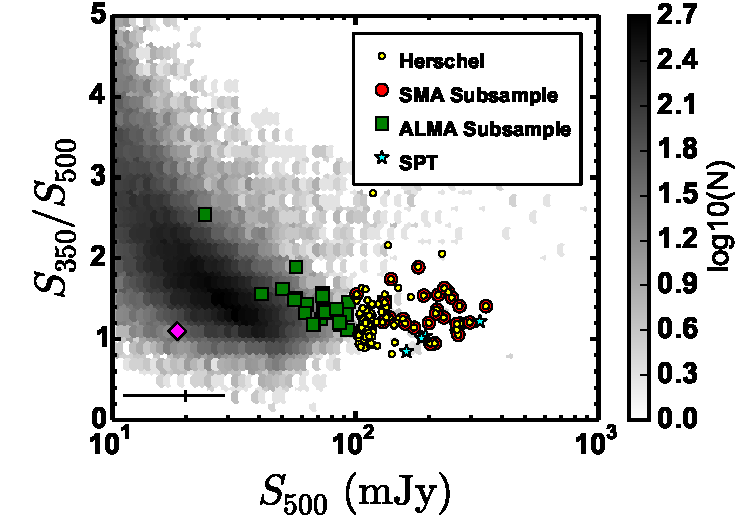
\includegraphics[width=\linewidth]{spirecolflux.pdf}

\caption{ {\it Herschel}/SPIRE photometry of all galaxies in the H-ATLAS
phase~I catalog with S/N$ > 3$ at 250$\,\mu$m, 350$\,\mu$m, and 500$\,\mu$m
(grayscale).  The sample of HerMES sources in this paper are shown with green
squares (the ``ALMA sample'').  The very bright {\it Herschel} DSFGs from
\citet{Bussmann:2013lr} (the ``SMA sample'') are shown by red circles, and the
overall sample of candidate lensed {\it Herschel} DSFGs are highlighted by
yellow circles.  Lensed SMGs discovered by the SPT that have published lens
models are represented by cyan stars \citep{Hezaveh:2013fk}.  A magenta diamond
shows the location in this diagram of the stacked signal from ALESS DSFGs.
Representative error bars are shown in the lower left corner.  The ALMA sample
fills the gap in 500$\,\mu$m flux density space between SMA/SPT and ALESS
samples.} \label{fig:sample}

\end{figure}

In detail, two of the sources in the ALMA sample (HXMM01 and HXMM02) overlap
with the ``confirmed lensed'' sample in \citet{Wardlow:2013lr} as well as with
the SMA sample in \citet{Bussmann:2013lr}.  A further 8 appear in the
``Supplementary sample'' in \citet{Wardlow:2013lr}.  The remainder have
$S_{500} < 80\,$mJy and thus do not appear in \citet{Wardlow:2013lr}.

%Efforts are on-going to obtain a complete database of follow-up observations
%for our ALMA sample.  The present paper focuses on a
%subset of 30 candidates with superb existing follow-up observations (hereafter,
%we refer to this as the ``SMA subsample'').  These targets were initially
%selected on the basis of strong 1.2$\,$mm detections from the Max Planck
%Millimeter Bolometer (MAMBO) array \citep{Kreysa:1998uq} at the Institut de
%Radioastronomie Millim\'etrique (IRAM) 30$\,$m telescope (Dannerbauer et al. in
%prep.).  Subsequent follow-up efforts have now provided high-spatial resolution
%880$\, \mu$m imaging with the SMA, spectroscopic redshifts of the lensed SMGs
%obtained with GBT, CSO, CARMA, PdBI, and {\it Herschel} \citep[][Riechers et
%al., in prep.; Krips et al., in prep., George et al., in prep.]{Cox:2011fk,
%Harris:2012fr, Lupu:2012ly}, and spectroscopic redshifts to the lenses obtained
%with the MMT, Gemini-S, or WHT.  In addition, Keck-II Near InfraRed Camera 2
%(NIRC2) laser guide star adaptive optics (LGSAO) imaging has been obtained for
%nearly half of the candidate lensed SMG sample \citep[][Calanog et al., in
%prep.]{Wardlow:2013lr}.  These datasets provide the information needed to
%confirm the lensing hypothesis and begin analysis of the source and lens
%properties.  

Table~\ref{tab:position} provides basic positional data for the ALMA sample,
including the International Astronomical Union addresses (for the full IAU
name, prepend ``1HerMES 250'' to the IAU address), short names to aid
comparison with previous publications, centroid positions measured from the
ALMA 870$\, \mu$m imaging (see section~\ref{sec:almaobs}), and redshift
measurements for the lens(es) and sources, where available.

\clearpage
\LongTables
\begin{deluxetable*}{llccccccc}[!tbp]
%\rotate
%\resizebox{\textwidth}{!}{%
\tabletypesize{\scriptsize}
\tablecolumns{9}
%\tablewidth{7.5in}
\tablecaption{Observed positions and flux densities of ALMA sources.
Uncertainties in flux densities do not include absolute calibration uncertainty
of $\approx 10\%$.}
%Definition of lens grades: \\
%Reference key: G05 = \citet{Gladders:2005qy}; B06 = \citet{Borys:2006lr}; N10 =
%\citet{Negrello:2010fk}; S11 = \citet{2011ApJ...733...29S}; F11 = \citet{2011ApJ...726L..22F}; C11 =
%\citet{Cox:2011fk}; H12 = \citet{Harris:2012fr}; B12 = \citet{Bussmann:2012lr};
%L12 = \citet{Lupu:2012ly}; W13 = \citet{Wardlow:2013lr}; I13 =
%\citet{Ivison:2013fk}; G13 = George et al. (in prep.); R13 = Riechers et al.
%(in prep.); K13 = Krips et al. (in prep.); L13 = Lupu et al. (in prep.); H13 = Harris et al. (in prep.).}
\tablehead{
\colhead{} & 
\colhead{} & 
\colhead{RA$_{870}$} &
\colhead{Dec$_{870}$} &
\colhead{$S_{250}$} &
\colhead{$S_{350}$} &
\colhead{$S_{500}$} &
\colhead{$S_{870}$} &
\colhead{Lens}
\\
\colhead{IAU address\tablenotemark{a}} & 
\colhead{Short name} & 
\colhead{(J2000)} &
\colhead{(J2000)} &
\colhead{(mJy)} &
\colhead{(mJy)} &
\colhead{(mJy)} &
\colhead{(mJy)} &
\colhead{Grade}
}
\startdata
J045057.5-531654              & ADFS01   & 04:50:57.715 & $-$53:16:54.42  &  $138   \pm  6 $  & $114   \pm  6 $  & $ 73   \pm  6  $  &   $10.41 \pm 0.44$ & --- \\
---                           & Source0  & 04:50:57.610 & $-$53:16:55.09  &         ---       &        ---       &        ---        &   $ 6.68 \pm 0.28$ & C   \\
---                           & Source1  & 04:50:57.805 & $-$53:16:56.96  &         ---       &        ---       &        ---        &   $ 1.98 \pm 0.18$ & C   \\
---                           & Source2  & 04:50:57.741 & $-$53:16:54.54  &         ---       &        ---       &        ---        &   $ 1.75 \pm 0.26$ & C   \\
J045026.5-524127              & ADFS02   & 04:50:27.453 & $-$52:41:25.41  &  $ 88   \pm  6 $  & $ 81   \pm  6 $  & $ 50   \pm  6  $  &   $10.39 \pm 0.42$ & --- \\
---                           & Source0  & 04:50:27.092 & $-$52:41:25.62  &         ---       &        ---       &        ---        &   $ 5.56 \pm 0.23$ & C   \\
---                           & Source1  & 04:50:27.806 & $-$52:41:25.10  &         ---       &        ---       &        ---        &   $ 4.83 \pm 0.35$ & X   \\
J044946.9-525424              & ADFS03   & 04:49:46.448 & $-$52:54:26.95  &  $115   \pm  6 $  & $ 61   \pm  6 $  & $ 24   \pm  6  $  &   $13.39 \pm 0.49$ & --- \\
---                           & Source0  & 04:49:46.603 & $-$52:54:23.66  &         ---       &        ---       &        ---        &   $ 7.50 \pm 0.24$ & X   \\
---                           & Source1  & 04:49:46.301 & $-$52:54:30.26  &         ---       &        ---       &        ---        &   $ 3.84 \pm 0.27$ & X   \\
---                           & Source2  & 04:49:46.280 & $-$52:54:26.06  &         ---       &        ---       &        ---        &   $ 2.06 \pm 0.30$ & X   \\
J044103.8-531240              & ADFS04   & 04:41:03.942 & $-$53:12:41.01  &  $ 96   \pm  6 $  & $ 86   \pm  6 $  & $ 57   \pm  6  $  &   $14.94 \pm 0.33$ & --- \\
---                           & Source0  & 04:41:03.866 & $-$53:12:41.33  &         ---       &        ---       &        ---        &   $ 8.65 \pm 0.23$ & X   \\
---                           & Source1  & 04:41:04.000 & $-$53:12:40.10  &         ---       &        ---       &        ---        &   $ 3.53 \pm 0.18$ & X   \\
---                           & Source2  & 04:41:03.912 & $-$53:12:42.09  &         ---       &        ---       &        ---        &   $ 2.76 \pm 0.16$ & X   \\
J043619.3-552425              & ADFS05   & 04:36:19.702 & $-$55:24:25.01  &  $110   \pm   6$  & $102   \pm 6  $  & $ 87   \pm  6  $  &   $15.29 \pm 0.37$ & --- \\
---                           & Source0  & 04:36:19.706 & $-$55:24:24.41  &         ---       &        ---       &        ---        &   $ 7.02 \pm 0.42$ & X   \\
---                           & Source1  & 04:36:19.698 & $-$55:24:25.27  &         ---       &        ---       &        ---        &   $ 8.27 \pm 0.53$ & X   \\
J043340.5-540337              & ADFS06   & 04:33:40.450 & $-$54:03:39.51  &  $ 76   \pm  6 $  & $ 90   \pm  6 $  & $ 72   \pm  6  $  &   $17.94 \pm 0.50$ & --- \\
---                           & Source0  & 04:33:40.455 & $-$54:03:40.29  &         ---       &        ---       &        ---        &   $ 9.07 \pm 0.27$ & C   \\
---                           & Source1  & 04:33:40.501 & $-$54:03:40.05  &         ---       &        ---       &        ---        &   $ 6.08 \pm 0.32$ & C   \\
---                           & Source2  & 04:33:40.472 & $-$54:03:38.33  &         ---       &        ---       &        ---        &   $ 2.79 \pm 0.27$ & C   \\
J044153.9-540350              & ADFS07   & 04:41:53.880 & $-$54:03:53.48  &  $  80  \pm   6$  & $103   \pm 6  $  & $ 93   \pm 6   $  &   $32.36 \pm 0.64$ & A   \\
J043829.7-541831              & ADFS\_M0 & 04:38:30.883 & $-$54:18:29.38  &  $  57  \pm   6$  & $ 78   \pm 5  $  & $ 75   \pm 6   $  &   $20.59 \pm 0.48$ & --- \\
---                           & Source0  & 04:38:30.780 & $-$54:18:31.79  &         ---       &        ---       &        ---        &   $14.00 \pm 0.40$ & C   \\
---                           & Source1  & 04:38:30.970 & $-$54:18:26.60  &         ---       &        ---       &        ---        &   $ 6.59 \pm 0.28$ & C   \\
J032752.0-290908              & CDFS\_M0 & 03:27:52.011 & $-$29:09:10.40  &  $  28  \pm   7$  & $ 84   \pm   6$  & $ 85   \pm 6   $  &   $33.16 \pm 0.45$ & --- \\
---                           & Source0  & 03:27:52.002 & $-$29:09:12.07  &         ---       &        ---       &        ---        &   $13.07 \pm 0.40$ & A   \\
---                           & Source1  & 03:27:52.002 & $-$29:09:09.65  &         ---       &        ---       &        ---        &   $14.26 \pm 0.22$ & C   \\
---                           & Source2  & 03:27:52.025 & $-$29:09:12.14  &         ---       &        ---       &        ---        &   $ 5.83 \pm 0.11$ & X   \\
J033210.8-270535              & CDFS\_M1 & 03:32:10.840 & $-$27:05:34.18  &  $  73  \pm   6$  & $ 86   \pm   6$  & $ 85  \pm  6   $  &   $13.12 \pm 0.25$ & --- \\
---                           & Source0  & 03:32:10.905 & $-$27:05:32.87  &         ---       &        ---       &        ---        &   $10.54 \pm 0.24$ & C   \\
---                           & Source1  & 03:32:10.729 & $-$27:05:36.22  &         ---       &        ---       &        ---        &   $ 2.58 \pm 0.11$ & C   \\
J033317.9-280907              & ECDFS02  & 03:33:18.017 & $-$28:09:07.52  &  $ 96   \pm  6 $  & $ 90   \pm  6 $  & $ 63   \pm  6  $  &   $14.13 \pm 0.25$ & --- \\
---                           & Source0  & 03:33:18.006 & $-$28:09:07.55  &         ---       &        ---       &        ---        &   $ 9.30 \pm 1.20$ & X   \\
---                           & Source1  & 03:33:18.032 & $-$28:09:07.39  &         ---       &        ---       &        ---        &   $ 4.83 \pm 1.26$ & X   \\
J100144.1+025712              & COS01    & 10:01:44.182 & $+$02:57:12.47  &  $ 91   \pm  6 $  & $100   \pm  6 $  & $ 74   \pm  6  $  &   $12.82 \pm 0.39$ & A   \\
J100056.6+022014              & COS02    & 10:00:57.180 & $+$02:20:12.70  &  $ 71   \pm  6 $  & $ 64   \pm  6 $  & $ 41   \pm  6  $  &   $10.37 \pm 0.51$ & --- \\
---                           & Source0  & 10:00:56.946 & $+$02:20:17.35  &         ---       &        ---       &        ---        &   $ 3.31 \pm 0.16$ & X   \\
---                           & Source1  & 10:00:57.565 & $+$02:20:11.26  &         ---       &        ---       &        ---        &   $ 2.26 \pm 0.19$ & X   \\
---                           & Source2  & 10:00:56.855 & $+$02:20:08.93  &         ---       &        ---       &        ---        &   $ 1.54 \pm 0.23$ & X   \\
---                           & Source3  & 10:00:57.274 & $+$02:20:12.66  &         ---       &        ---       &        ---        &   $ 1.45 \pm 0.18$ & X   \\
---                           & Source4  & 10:00:57.400 & $+$02:20:10.83  &         ---       &        ---       &        ---        &   $ 1.80 \pm 0.33$ & X   \\
J003823.6-433707              & ElaisS1  & 00:38:23.587 & $-$43:37:04.15  &  $114   \pm  6 $  & $101   \pm  6 $  & $ 76   \pm  6  $  &   $17.20 \pm 0.44$ & --- \\
---                           & Source0  & 00:38:23.762 & $-$43:37:06.10  &         ---       &        ---       &        ---        &   $ 8.85 \pm 0.21$ & C   \\
---                           & Source1  & 00:38:23.482 & $-$43:37:05.56  &         ---       &        ---       &        ---        &   $ 3.76 \pm 0.19$ & C   \\
---                           & Source2  & 00:38:23.313 & $-$43:36:58.97  &         ---       &        ---       &        ---        &   $ 2.84 \pm 0.23$ & C   \\
---                           & Source3  & 00:38:23.803 & $-$43:37:10.46  &         ---       &        ---       &        ---        &   $ 1.75 \pm 0.20$ & X   \\
J022016.5-060143              & XMM01    & 02:20:16.609 & $-$06:01:43.18  &  $180   \pm   7$  & $192   \pm 8  $  & $132   \pm  7  $  &   $25.09 \pm 0.51$ & --- \\
---                           & Source0  & 02:20:16.648 & $-$06:01:41.93  &         ---       &        ---       &        ---        &   $13.77 \pm 0.34$ & C   \\
---                           & Source1  & 02:20:16.571 & $-$06:01:44.56  &         ---       &        ---       &        ---        &   $10.56 \pm 0.37$ & C   \\
---                           & Source2  & 02:20:16.609 & $-$06:01:40.72  &         ---       &        ---       &        ---        &   $ 0.76 \pm 0.32$ & C   \\
J022201.6-033340              & XMM02    & 02:22:01.616 & $-$03:33:41.40  &  $107   \pm   7$  & $108   \pm 8  $  & $ 81   \pm  7  $  &   $11.57 \pm 0.56$ & --- \\
---                           & Source0  & 02:22:01.592 & $-$03:33:39.42  &         ---       &        ---       &        ---        &   $ 8.45 \pm 0.38$ & C   \\
---                           & Source1  & 02:22:01.629 & $-$03:33:43.58  &         ---       &        ---       &        ---        &   $ 3.12 \pm 0.41$ & X   \\
J022548  -041750              & XMM03    & 02:25:47.942 & $-$04:17:50.80  &  $106   \pm   7$  & $119   \pm 8  $  & $ 92   \pm  7  $  &   $14.73 \pm 0.35$ & C  \\
J021853.1-063325              & XMM04    & 02:18:53.111 & $-$06:33:24.65  &  $ 89   \pm  7 $  & $ 83   \pm  7 $  & $ 56   \pm  7  $  &   $ 7.25 \pm 0.44$ & --- \\
---                           & Source0  & 02:18:53.118 & $-$06:33:24.19  &         ---       &        ---       &        ---        &   $ 5.46 \pm 0.30$ & C   \\
---                           & Source1  & 02:18:53.095 & $-$06:33:25.21  &         ---       &        ---       &        ---        &   $ 1.78 \pm 0.37$ & C   \\
J023006.0-034152              & XMM05    & 02:30:05.950 & $-$03:41:53.07  &  $102   \pm 7  $  & $110   \pm 8  $  & $ 81   \pm  7  $  &   $16.34 \pm 0.37$ & C   \\
J021830.5-053124              & XMM06    & 02:18:30.673 & $-$05:31:31.75  &  $ 92   \pm 7  $  & $122   \pm 8  $  & $113   \pm  7  $  &   $62.06 \pm 0.57$ & A   \\
J022135.1-062617              & XMM16    & 02:21:34.891 & $-$06:26:17.87  &  $121   \pm   7$  & $132   \pm 8  $  & $110   \pm  7  $  &   $18  8 \pm 0.41$ & C   \\
J022250.5-032410              & XMM101   & 02:22:50.573 & $-$03:24:12.35  &  $ 97   \pm  7 $  & $ 82   \pm  7 $  & $ 62   \pm  7  $  &   $ 8.77 \pm 0.24$ & C   \\
J021942.7-052436              & XMM102   & 02:19:42.783 & $-$05:24:34.84  &  $ 85   \pm  7 $  & $ 79   \pm  7 $  & $ 67   \pm  7  $  &   $14.21 \pm 0.61$ & --- \\
---                           & Source0  & 02:19:42.629 & $-$05:24:37.11  &         ---       &        ---       &        ---        &   $ 5.15 \pm 0.32$ & X   \\
---                           & Source1  & 02:19:42.838 & $-$05:24:35.11  &         ---       &        ---       &        ---        &   $ 3.31 \pm 0.39$ & X   \\
---                           & Source2  & 02:19:42.769 & $-$05:24:36.48  &         ---       &        ---       &        ---        &   $ 2.88 \pm 0.22$ & X   \\
---                           & Source3  & 02:19:42.682 & $-$05:24:36.82  &         ---       &        ---       &        ---        &   $ 1.94 \pm 0.37$ & X   \\
---                           & Source4  & 02:19:42.955 & $-$05:24:32.22  &         ---       &        ---       &        ---        &   $ 0.94 \pm 0.18$ & X   \\
J021918.4-031051              & XMM108   & 02:19:18.417 & $-$03:10:51.35  &  $ 91   \pm   7$  & $104   \pm 8  $  & $ 86   \pm  7  $  &   $29.16 \pm 0.58$ & A   \\
J022944.7-034110              & XMM109   & 02:29:44.740 & $-$03:41:09.57  &  $ 90   \pm  7 $  & $100   \pm  7 $  & $ 75   \pm  7  $  &   $23.13 \pm 0.41$ & --- \\
---                           & Source0  & 02:29:44.701 & $-$03:41:09.29  &         ---       &        ---       &        ---        &   $19.62 \pm 0.27$ & C   \\
---                           & Source1  & 02:29:44.793 & $-$03:41:09.92  &         ---       &        ---       &        ---        &   $ 3.51 \pm 0.30$ & C   \\
J021841.5-035002              & XMM110   & 02:18:41.613 & $-$03:50:03.70  &  $128   \pm  7 $  & $112   \pm  7 $  & $ 73   \pm  7  $  &   $10.13 \pm 0.43$ & --- \\
---                           & Source0  & 02:18:41.520 & $-$03:50:04.72  &         ---       &        ---       &        ---        &   $ 6.31 \pm 0.34$ & X   \\
---                           & Source1  & 02:18:41.700 & $-$03:50:02.57  &         ---       &        ---       &        ---        &   $ 3.81 \pm 0.25$ & C   \\
J022021.7-015328              & XMM115   & 02:20:21.756 & $-$01:53:30.92  &  $144   \pm   7$  & $137   \pm 8  $  & $ 93   \pm 11  $  &   $17.61 \pm 0.49$ & C   \\
J022029.2-064845              & XMM119   & 02:20:29.140 & $-$06:48:46.49  &  $120   \pm   7$  & $115   \pm 8  $  & $ 84   \pm  7  $  &   $14.46 \pm 0.37$ & --- \\
---                           & Source0  & 02:20:29.195 & $-$06:48:48.02  &         ---       &        ---       &        ---        &   $ 8.47 \pm 0.30$ & C   \\
---                           & Source1  & 02:20:29.079 & $-$06:48:44.86  &         ---       &        ---       &        ---        &   $ 5.98 \pm 0.18$ & C   \\
J022205.4-070728              & XMM124   & 02:22:05.362 & $-$07:07:28.10  &  $137   \pm  7 $  & $108   \pm  7 $  & $ 57   \pm  7  $  &   $2.75  \pm 0.14$ & X   \\
\enddata
\label{tab:position}
%\tnt{a}{Multiple lens redshifts have been measured for these targets.  The redshift uncertainty is 0.001 in all cases.}
\tablenotetext{a}{IAU name = 1HerMES S250 + IAU address}
%\tablenotetext{c}{WHT/ACAM?}
%\tablenotetext{d}{\citet{Bussmann:2012lr}}
% 
%\tablenotetext{a}{\citet{Lupu:2012ly}}
%\tablenotetext{b}{\citet{Harris:2012fr}}
%\tablenotetext{c}{\citet{2011ApJ...726L..22F}}
%\tablenotetext{d}{Riechers et al., in prep.}
%\tablenotetext{e}{Krips et al., in prep.}
%\tablenotetext{f}{\citet{Cox:2011fk}}
%\tablenotetext{g}{George et al., in prep.}
%%\tablenotetext{h}{\citep{Wardlow:2013lr}}
\end{deluxetable*}


\subsection{ALMA Observations}\label{sec:almaobs}

ALMA data were obtained during Cycle~0 over a period from 2012 June to 2012
December (Program 2011.0.00539.S; PI: D. Riechers).  The observations were
carried out in good 870$\,\mu$m weather conditions which resulted in typical
system temperatures of $T_{\rm sys} \sim 130\,$K and phase fluctuations of
$\sim 10\,$deg.  Each target was observed until an rms noise level of $\sigma
\approx 0.2\,$mJy was achieved.  This typically required 10 minutes of
on-source integration time.  The number of antennas used varied from 15 to 25.
The antennas were configured with baseline lengths of 20$\,$m to 400$\,$m,
providing a synthesized beamsize of $\approx 0\farcs45$ FWHM while ensuring
that no flux was resolved out by the interferometer.  When possible,
track-sharing of multiple targets in a single track was used to optimize the
{\it uv} coverage.

The quasars J0403$-$360, J2258$-$279, B0851$+$202, and J2258$-$279 were used
for bandpass and pointing calibration.  The quasars J0403$-$360, J0106$-$405,
J0519$-$454, J1008$+$063, and J0217$+017$ were used for amplitude and phase
gain calibration.  The following solar system objects were used for absolute
flux calibration: Callisto (CDFS targets), Neptune (XMM targets), Titan (COSMOS
targets) and Uranus (ADFS and XMM targets).  For ElaisS1, no solar system
object was observed.  Instead, J2258$-$279 was used for absolute flux
calibration, with the flux fixed according to a measurement made two days prior
to the observations of ElaisS1.

All observations were conducted with the correlator in ``Frequency Domain
Mode'', providing a total usable bandwidth of 7.5$\,$GHz with spectral windows
centered on 335.995$\,$GHz, 337.995$\,$GHz, 345.995$\,$GHz, 347.996$\,$GHz.  We
searched for evidence of serendipitous spectral lines but found none.

We used the Common Astronomy Software Applications (CASA, version 4.2.1)
package to investigate the quality of the reduced data provided by the North
American ALMA Science Center (NAASC).  Overall, the quality of the processed
data from the NAASC was very high.  We achieved a significant improvement in
the case of the ADFS and XMM targets by excluding datasets with moderate
$T_{\rm sys}$ and poor phase fluctuations.  For a handful of targets with peak
signal-to-noise ratio (S/N) greater than 20, we obtained a $\approx 10\%$
improvement in S/N by using the CASA {\sc selfcal} task to improve the phase
gain corrections.  Finally, we updated the absolute flux calibration to use the
Butler-JPL-Horizons 2012 solar system models.

For imaging, we used the CASA {\sc Clean} task with Briggs weighting and robust
= $+$0.5 to achieve the optimal balance between sensitivity and spatial
resolution.  We selected the multi-frequency synthesis option to optimize {\it
uv} coverage.  We designed custom masks for each target in CASA to ensure that
only regions with high S/N were considered during the cleaning process.

Figure~\ref{fig:imaging} presents our ALMA images (colorscale) in comparison to
the {\it Herschel} SPIRE images (black-white contours) originally used to
select the targets and noted in each panel as either 250$\,\mu$m or
350$\,\mu$m.  Each panel is centered on the phase center of the ALMA
observations of that target and a white circle traces the FWHM of the primary
beam of an ALMA 12$\,$m antenna at 870$\,\mu$m.  A white dashed box represents
the region of each image that is shown in greater detail in
Figure~\ref{fig:uvmodels}.

\begin{figure*}[!tbp] 
    \begin{centering}
%\epsscale{1.00} 
%\includegraphics[width=\textwidth]{cutouts_dec17.png}
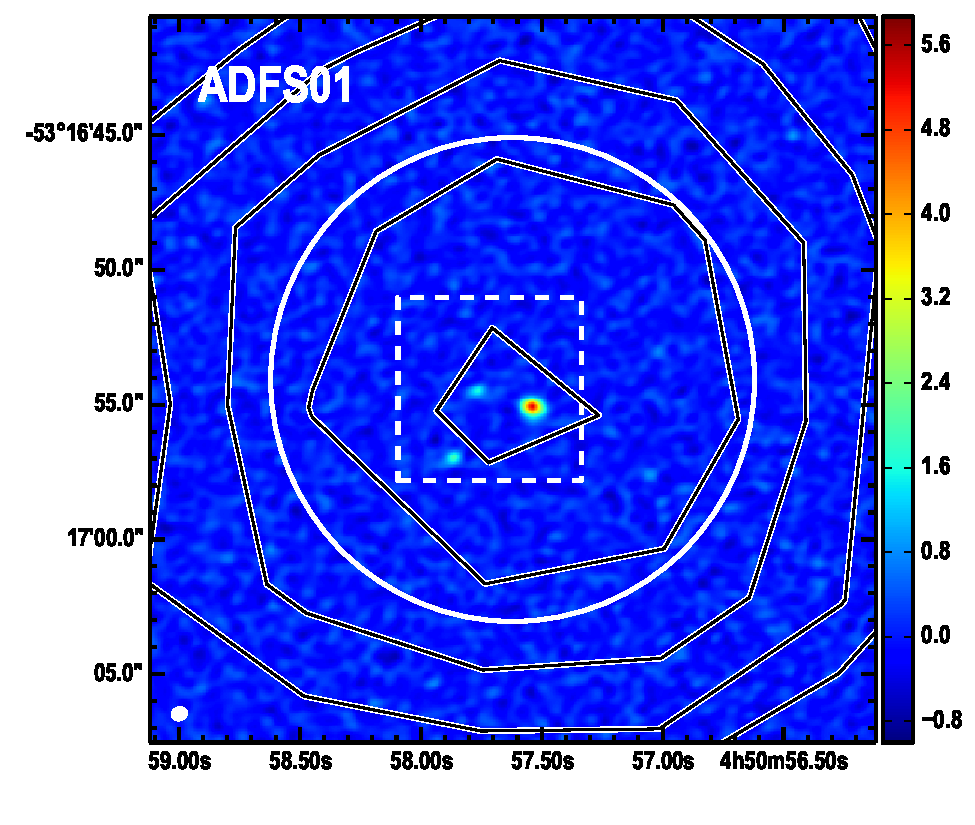
\includegraphics[width=0.245\textwidth]{overlays/ADFS01_870_250.pdf}
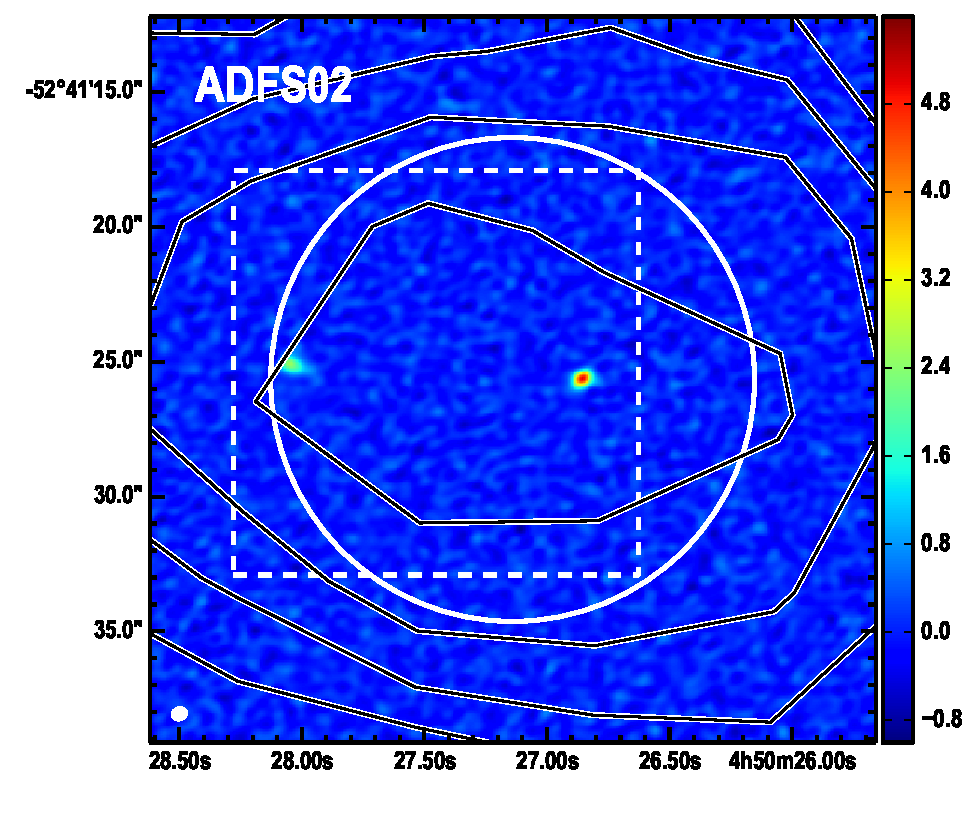
\includegraphics[width=0.245\textwidth]{overlays/ADFS02_870_250.pdf}
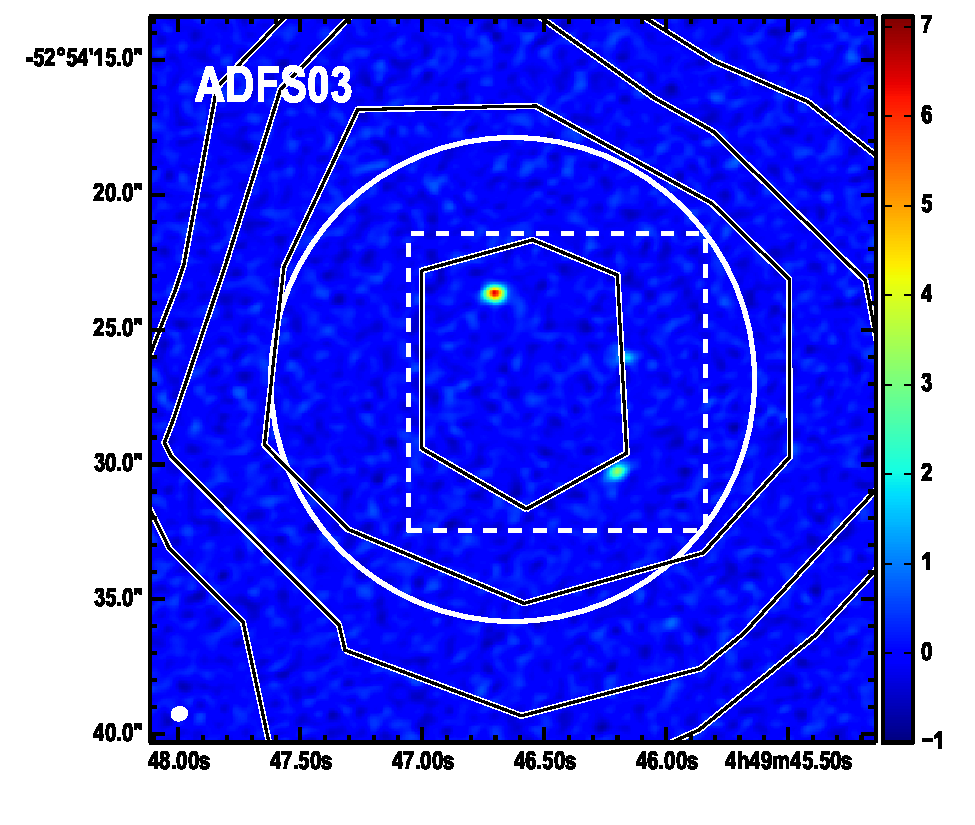
\includegraphics[width=0.245\textwidth]{overlays/ADFS03_870_250.pdf}
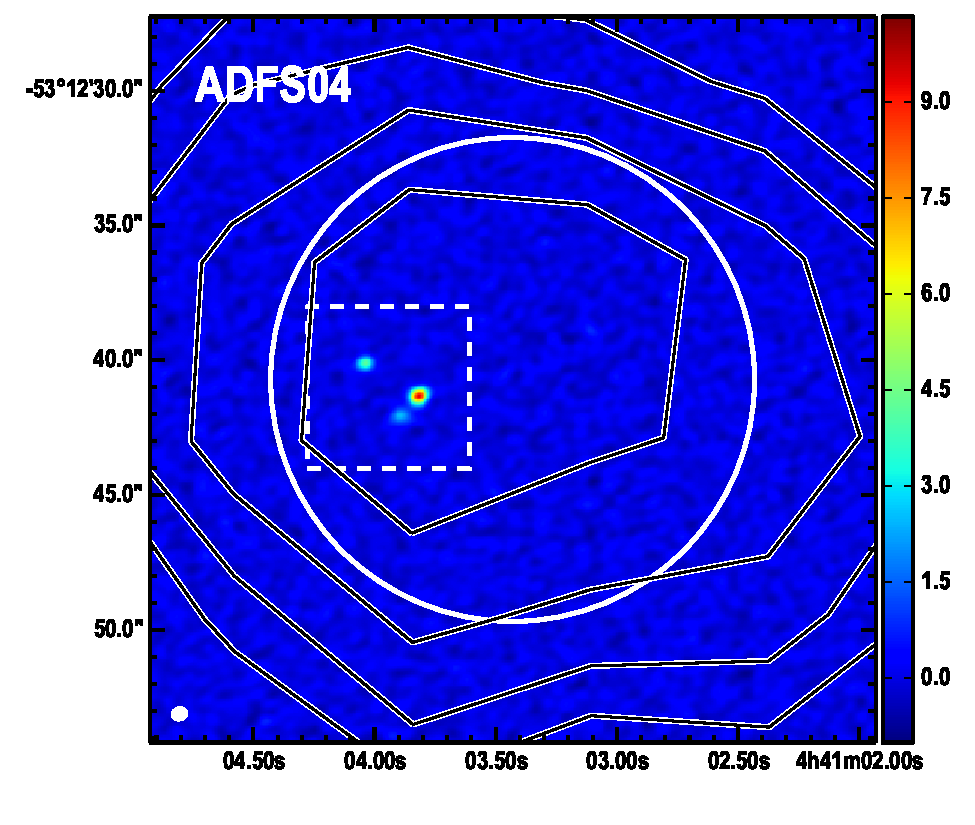
\includegraphics[width=0.245\textwidth]{overlays/ADFS04_870_250.pdf}
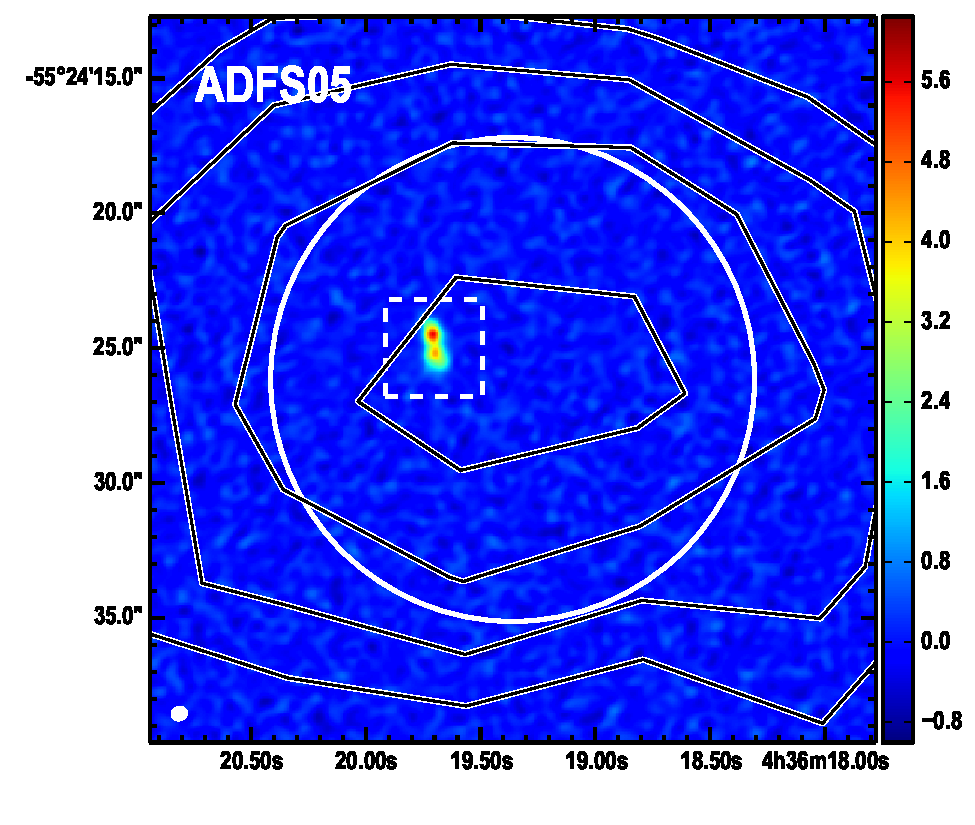
\includegraphics[width=0.245\textwidth]{overlays/ADFS05_870_250.pdf}
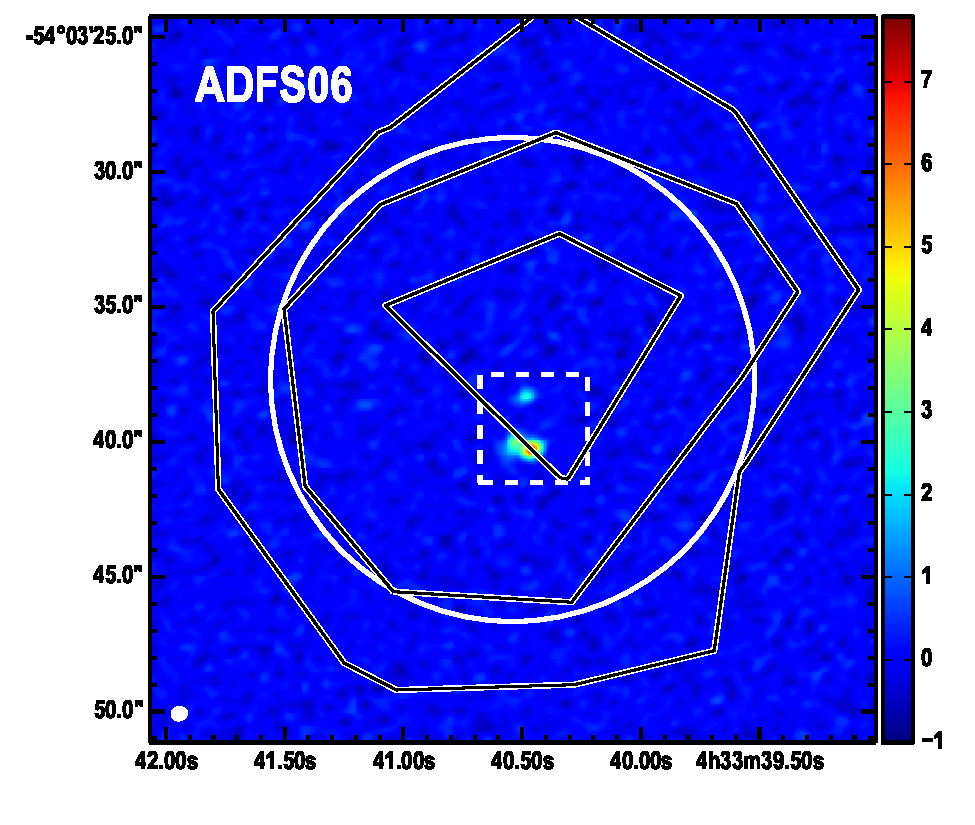
\includegraphics[width=0.245\textwidth]{overlays/ADFS06_870_250.pdf}
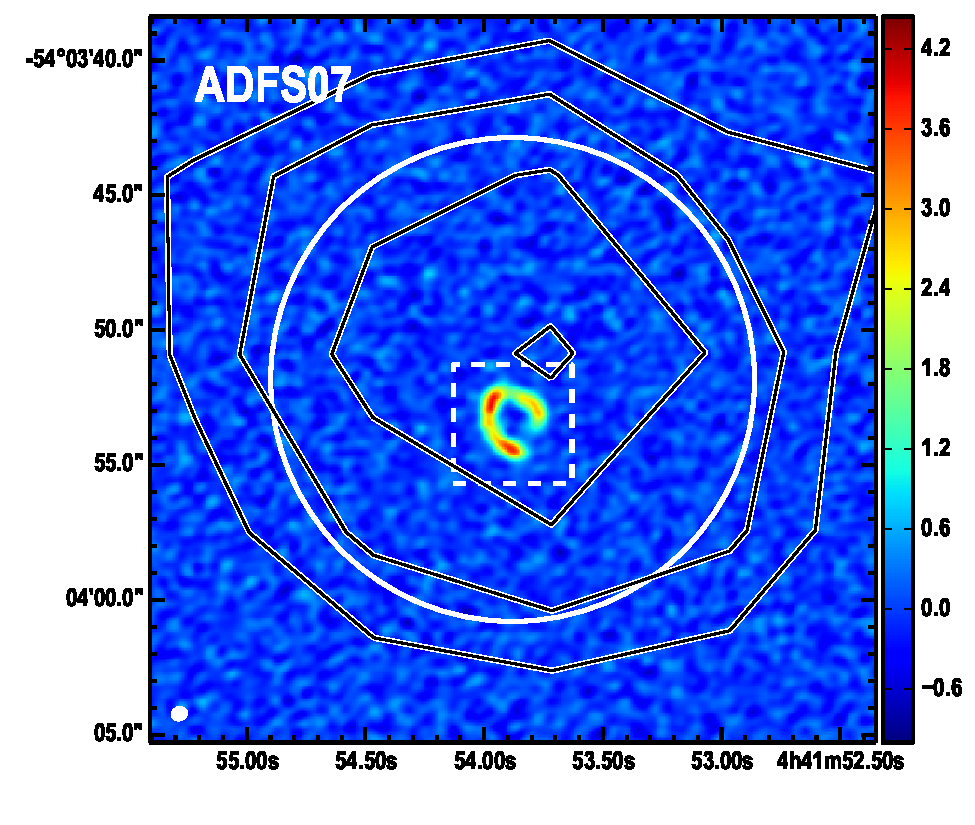
\includegraphics[width=0.245\textwidth]{overlays/ADFS07_870_250.pdf}
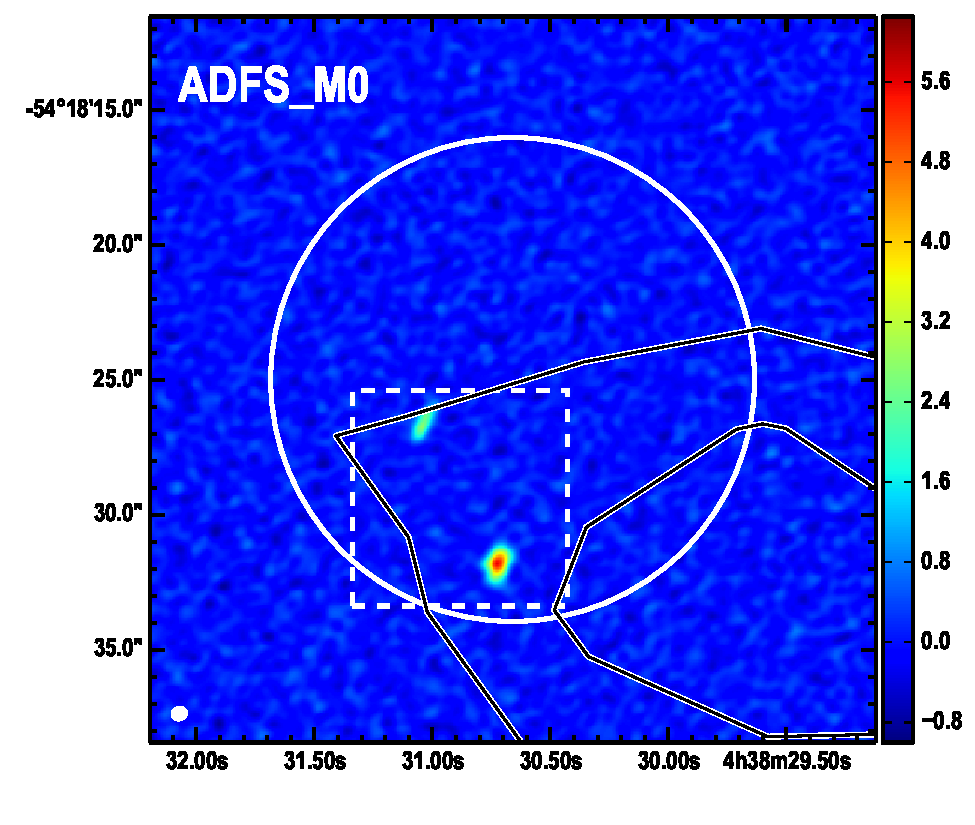
\includegraphics[width=0.245\textwidth]{overlays/ADFS_M0_870_250.pdf}
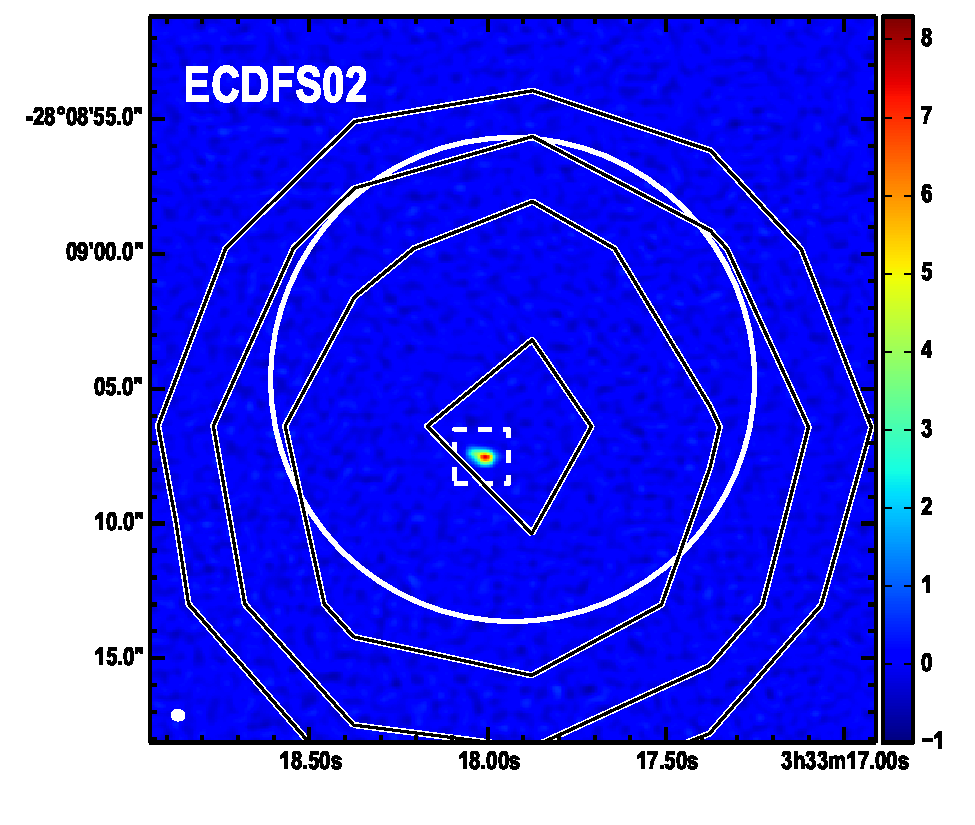
\includegraphics[width=0.245\textwidth]{overlays/ECDFS02_870_250.pdf}
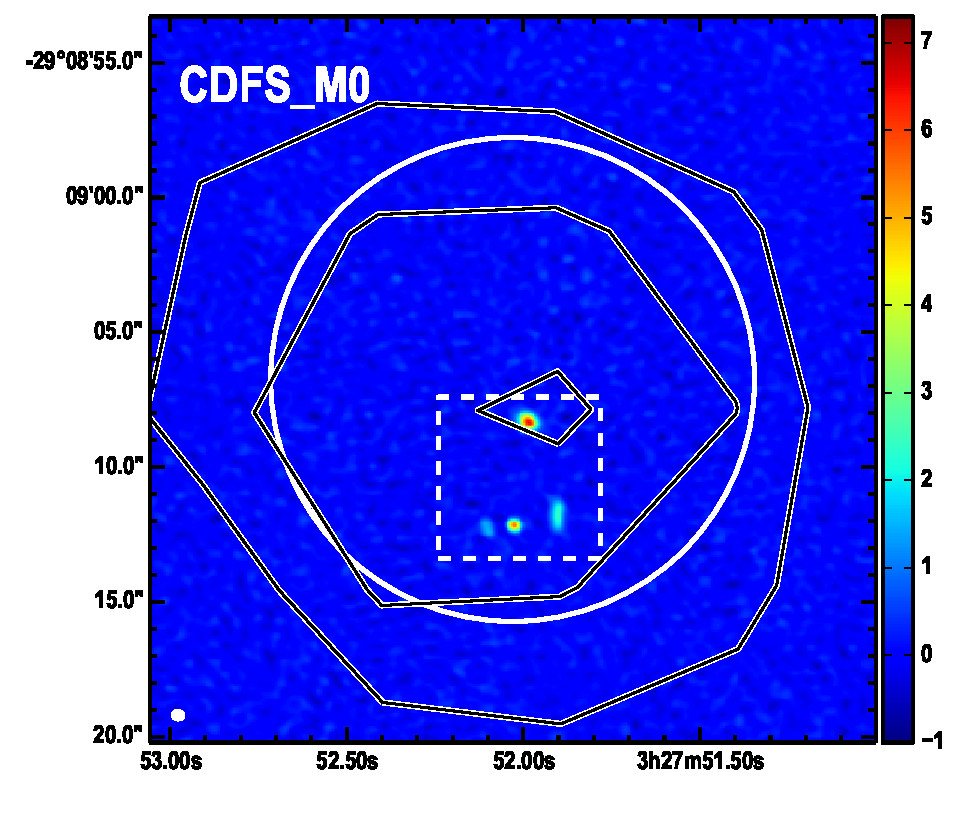
\includegraphics[width=0.245\textwidth]{overlays/CDFS_M0_870_250.pdf}
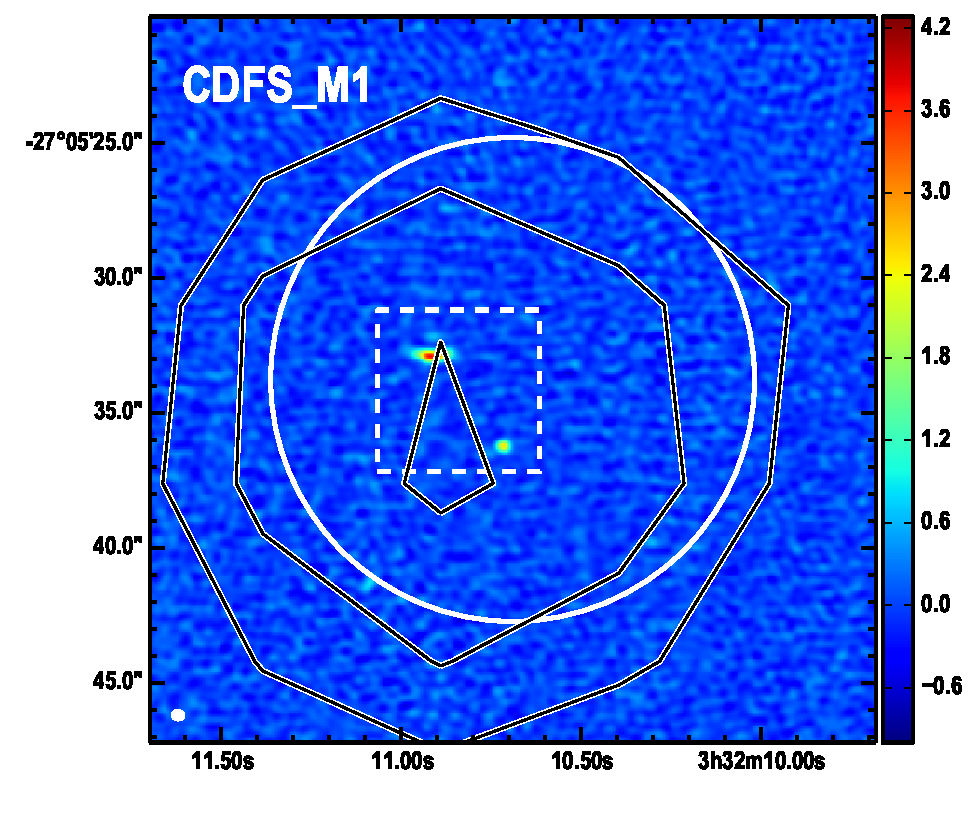
\includegraphics[width=0.245\textwidth]{overlays/CDFS_M1_870_250.pdf}
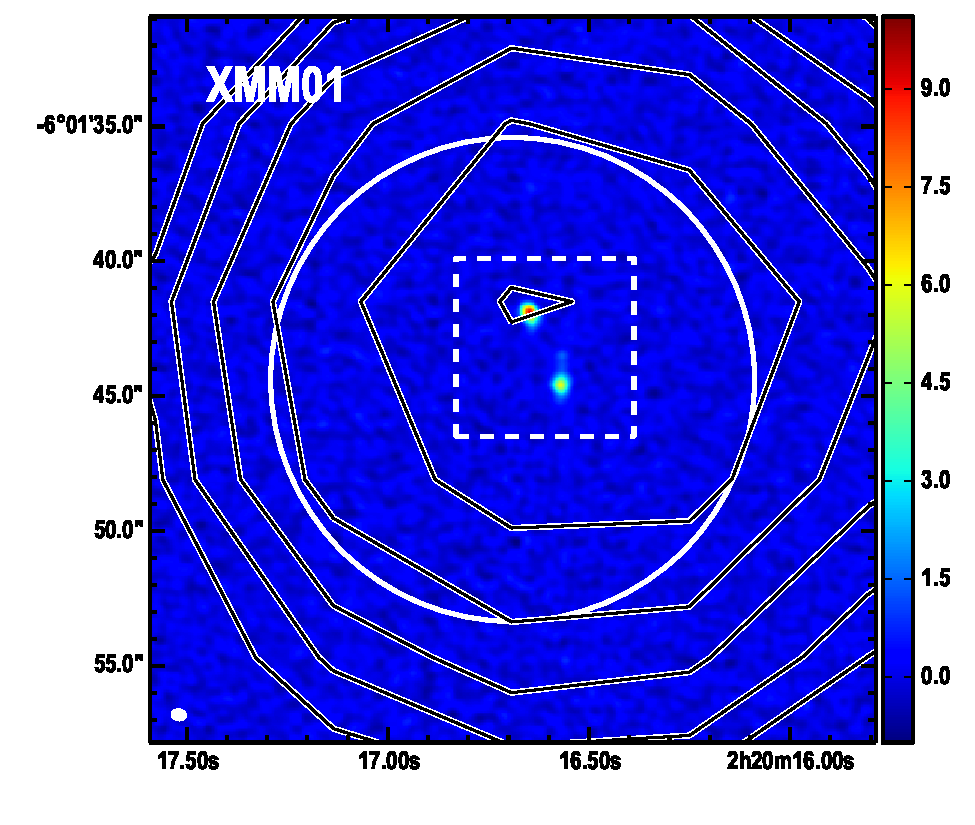
\includegraphics[width=0.245\textwidth]{overlays/XMM01_870_250.pdf}
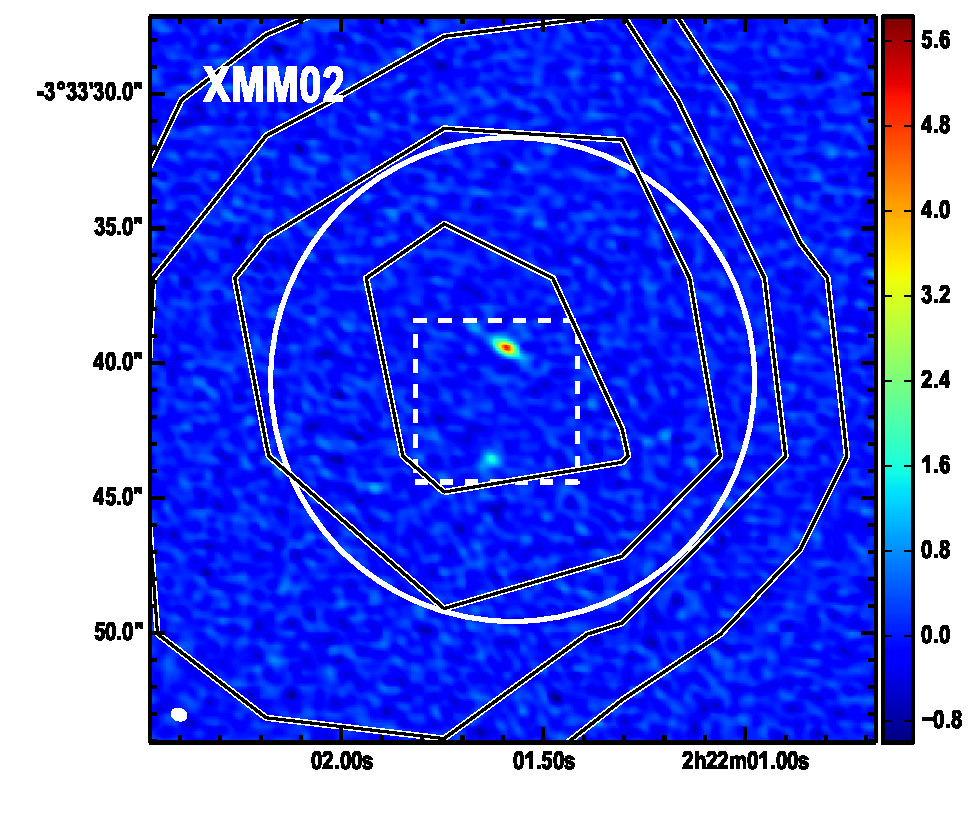
\includegraphics[width=0.245\textwidth]{overlays/XMM02_870_250.pdf}
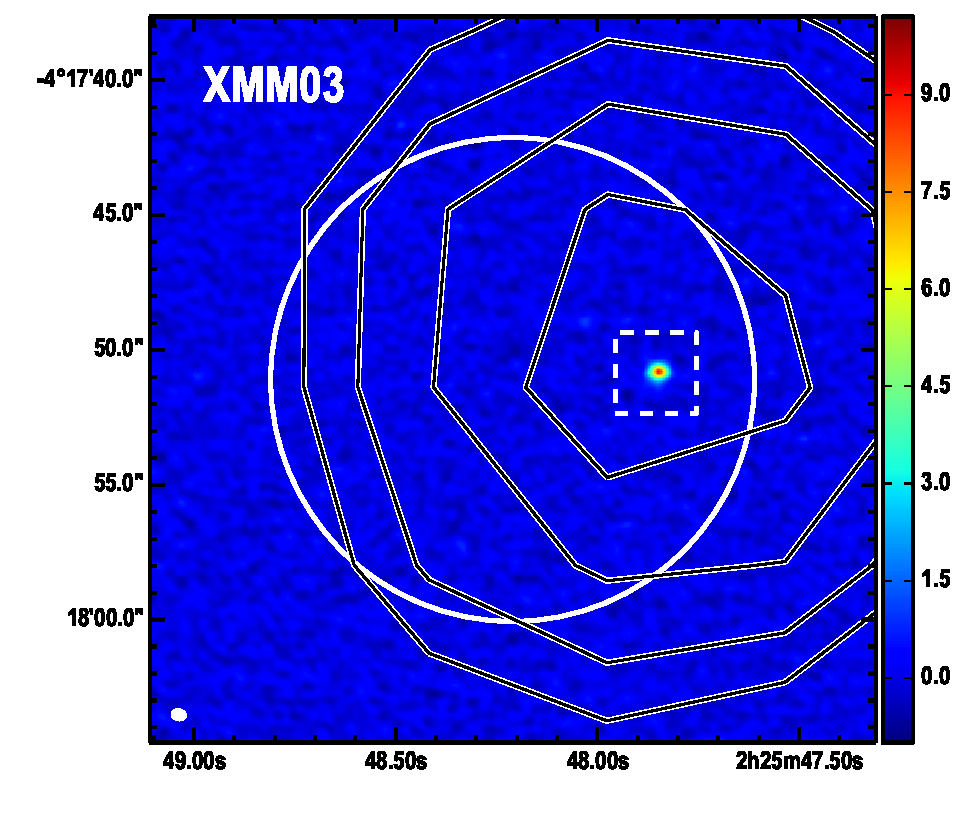
\includegraphics[width=0.245\textwidth]{overlays/XMM03_870_250.pdf}
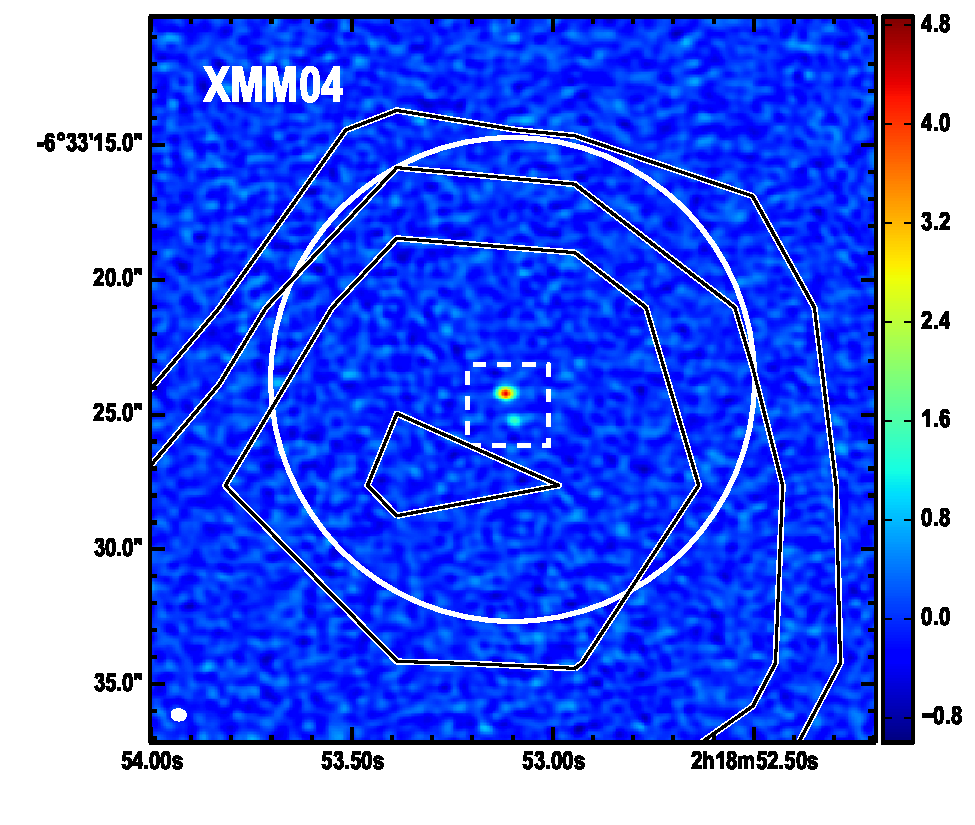
\includegraphics[width=0.245\textwidth]{overlays/XMM04_870_250.pdf}
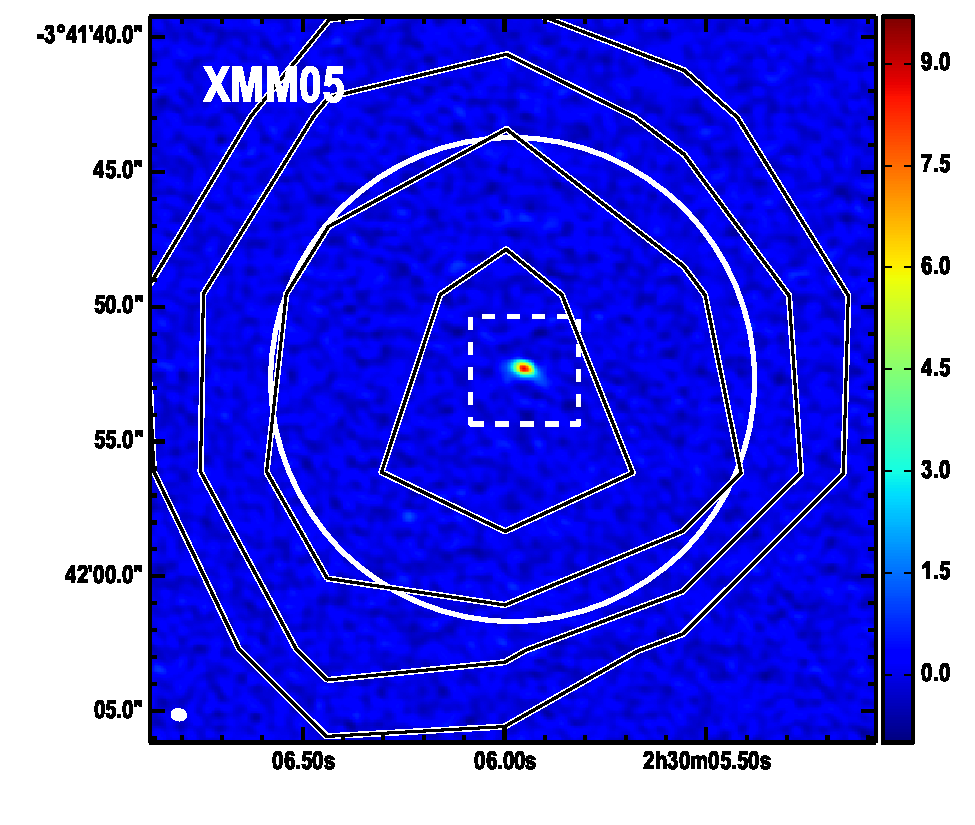
\includegraphics[width=0.245\textwidth]{overlays/XMM05_870_250.pdf}
\end{centering}

\caption{ ALMA 870$\mu$m images (color scale, units of mJy/beam) of HerMES
DSFGs.  Contours (black and white) trace 250$\,\mu$m emission from {\it
Herschel}.  The FWHM size of the ALMA synthesized beam is shown in the lower
left corner of each panel.  A solid white circle shows the FWHM size of the
primary beam.  Dashed squares identify the regions of each image that are shown
in greater detail in Figure~\ref{fig:uvmodels}.  \label{fig:imaging}}
\addtocounter{figure}{-1}

\end{figure*}


%\begin{figure*}[!tbp] 
%    \begin{centering}
%%\epsscale{1.00} 
%%\includegraphics[width=\textwidth]{cutouts_dec17.png}
%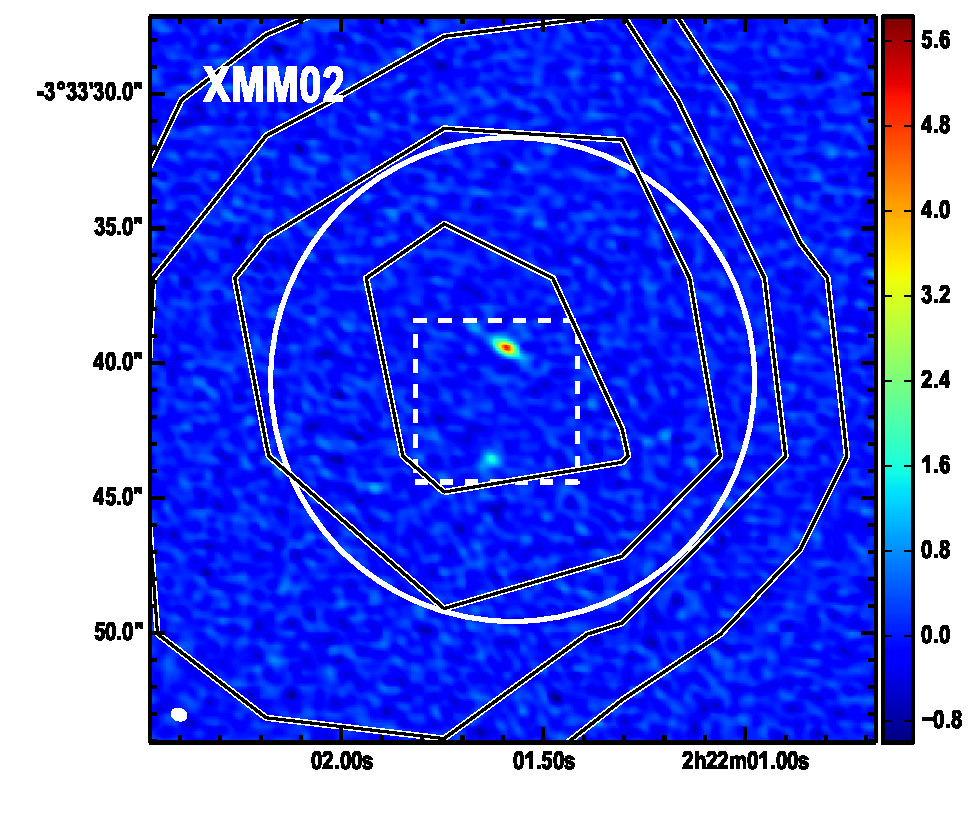
\includegraphics[width=0.245\textwidth]{overlays/XMM02_870_250.pdf}
%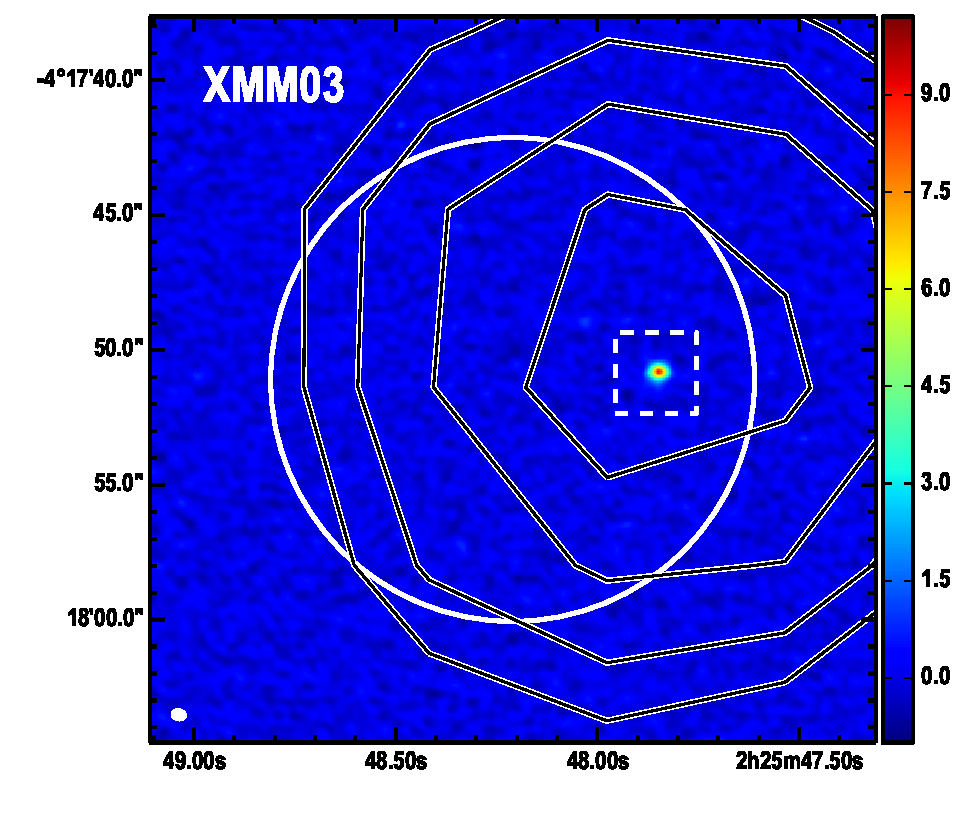
\includegraphics[width=0.245\textwidth]{overlays/XMM03_870_250.pdf}
%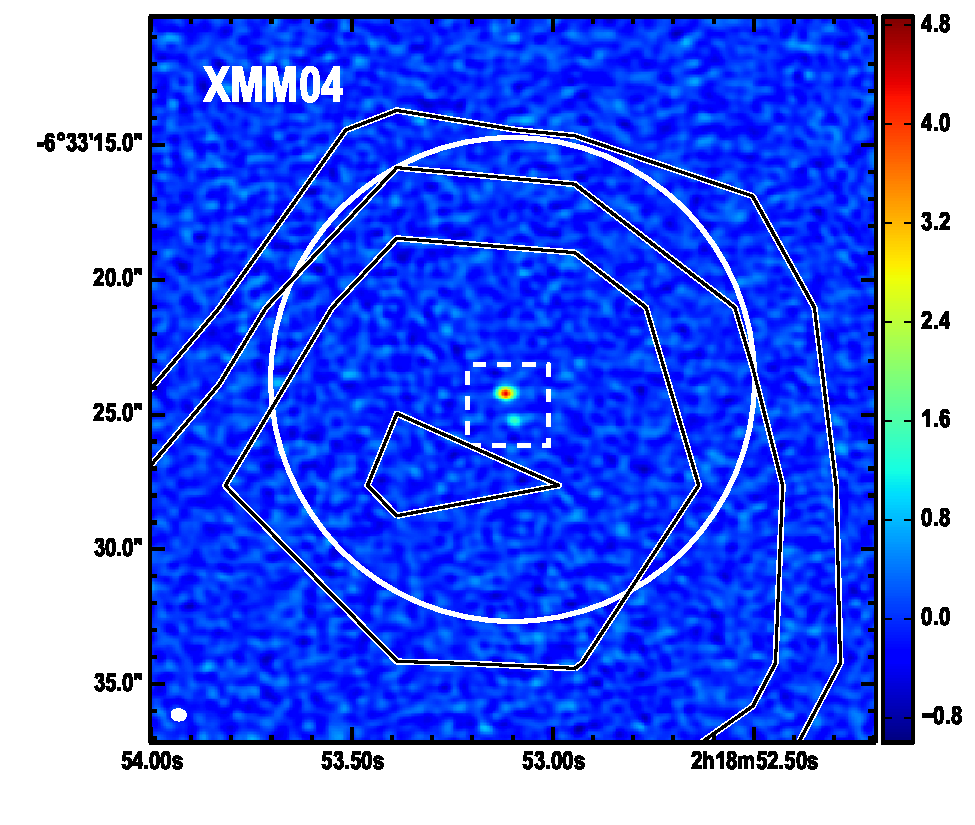
\includegraphics[width=0.245\textwidth]{overlays/XMM04_870_250.pdf}
%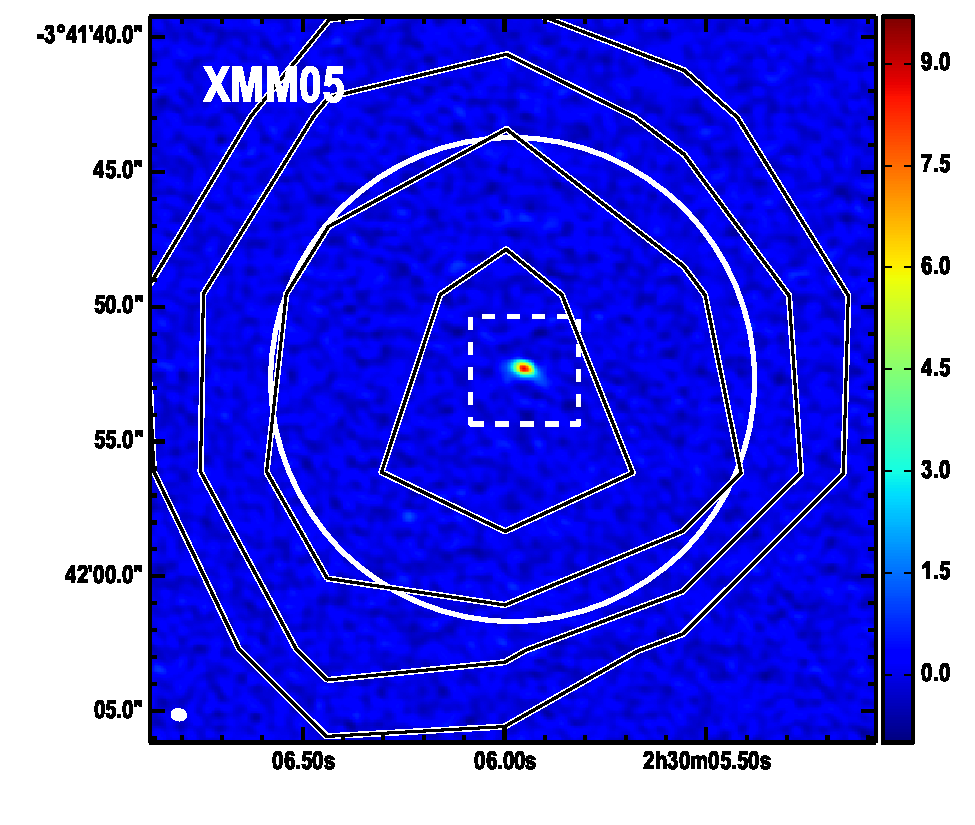
\includegraphics[width=0.245\textwidth]{overlays/XMM05_870_250.pdf}
%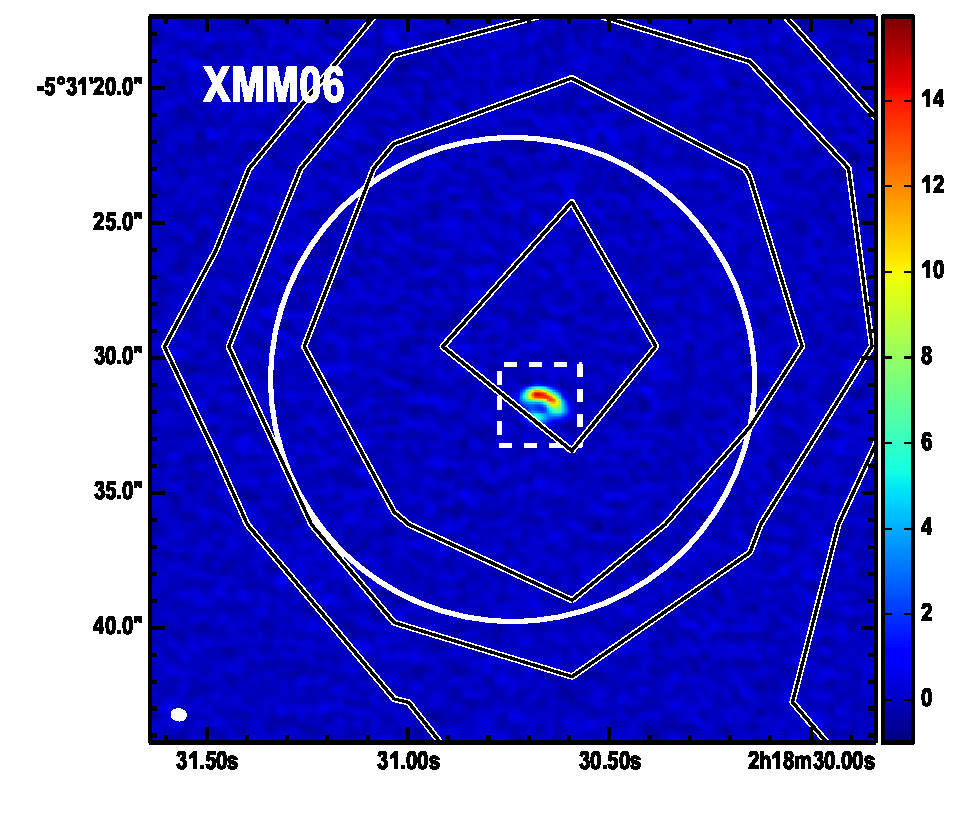
\includegraphics[width=0.245\textwidth]{overlays/XMM06_870_250.pdf}
%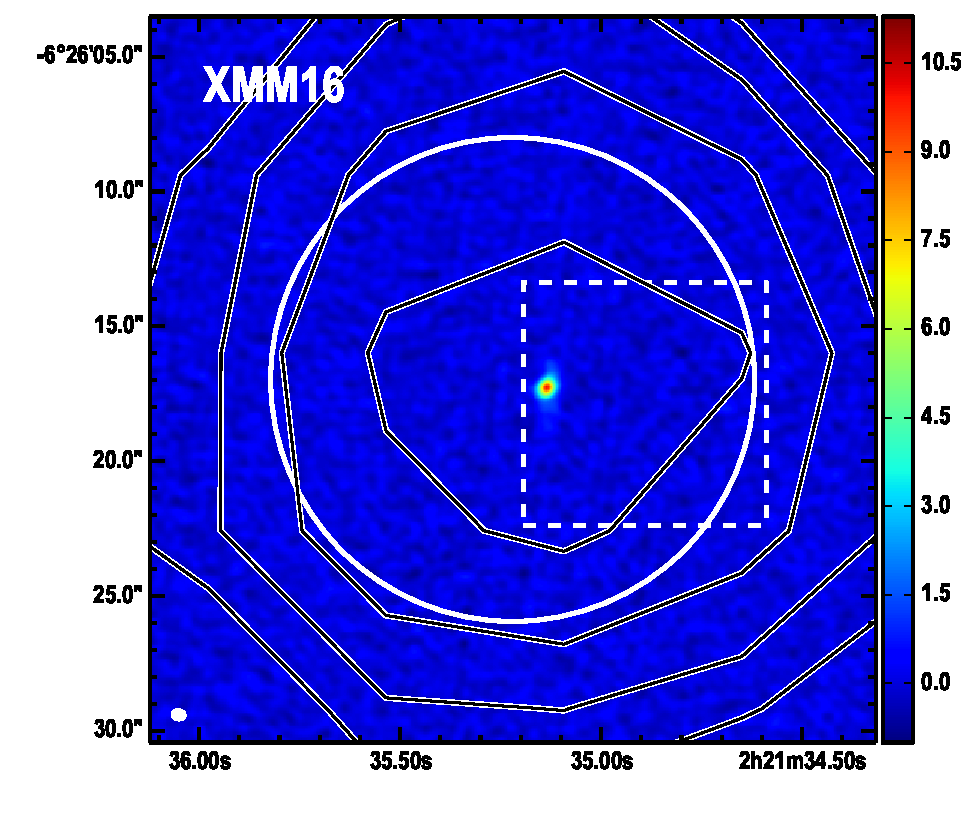
\includegraphics[width=0.245\textwidth]{overlays/XMM16_870_250.pdf}
%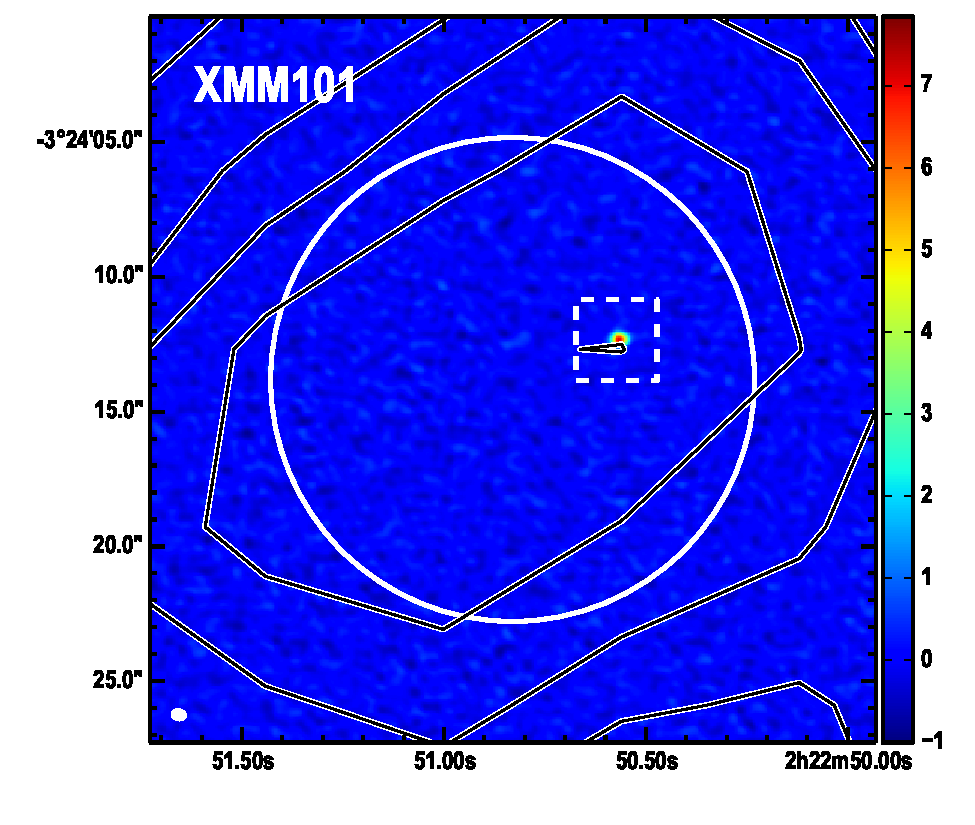
\includegraphics[width=0.245\textwidth]{overlays/XMM101_870_250.pdf}
%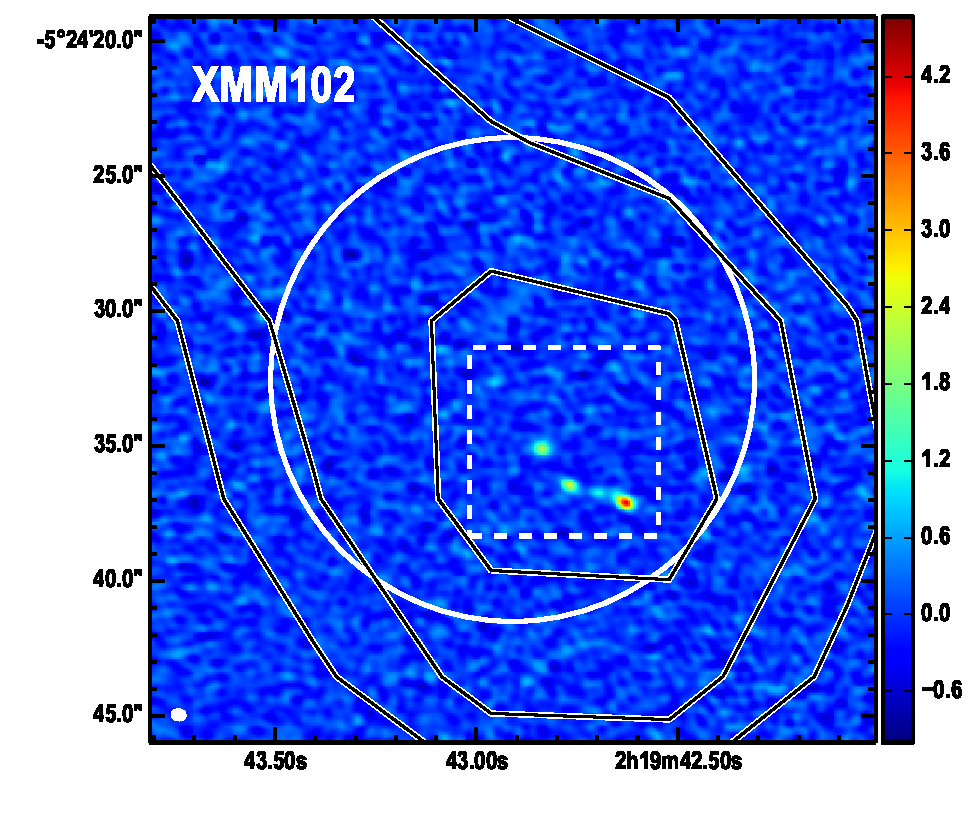
\includegraphics[width=0.245\textwidth]{overlays/XMM102_870_250.pdf}
%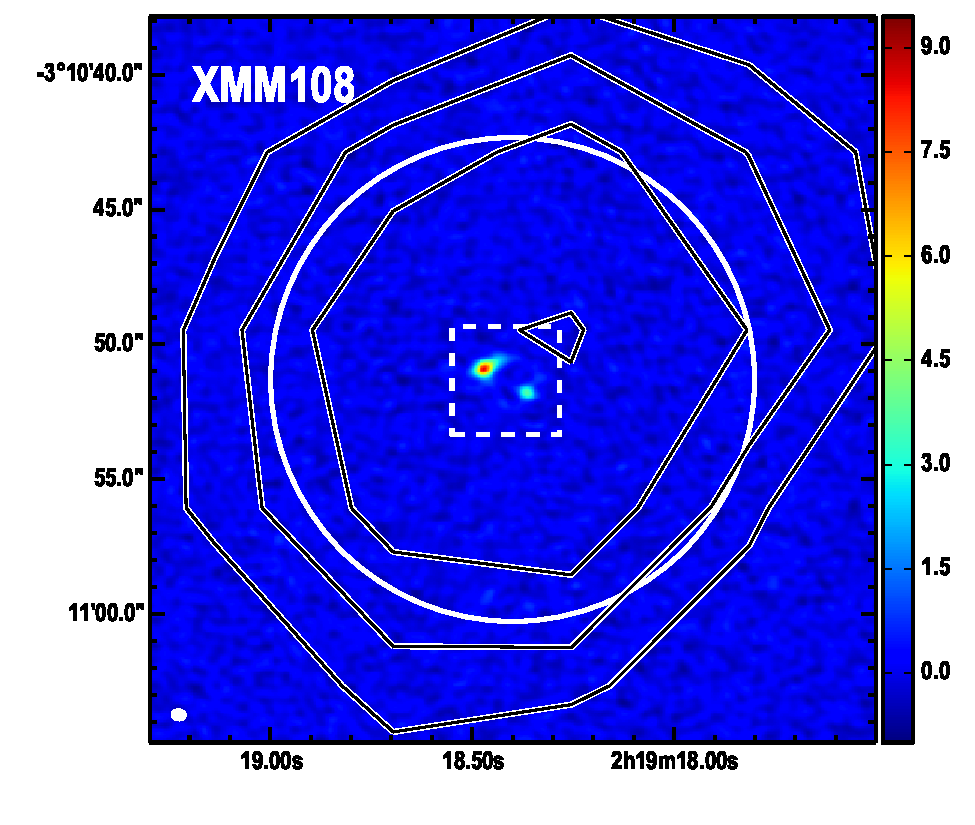
\includegraphics[width=0.245\textwidth]{overlays/XMM108_870_250.pdf}
%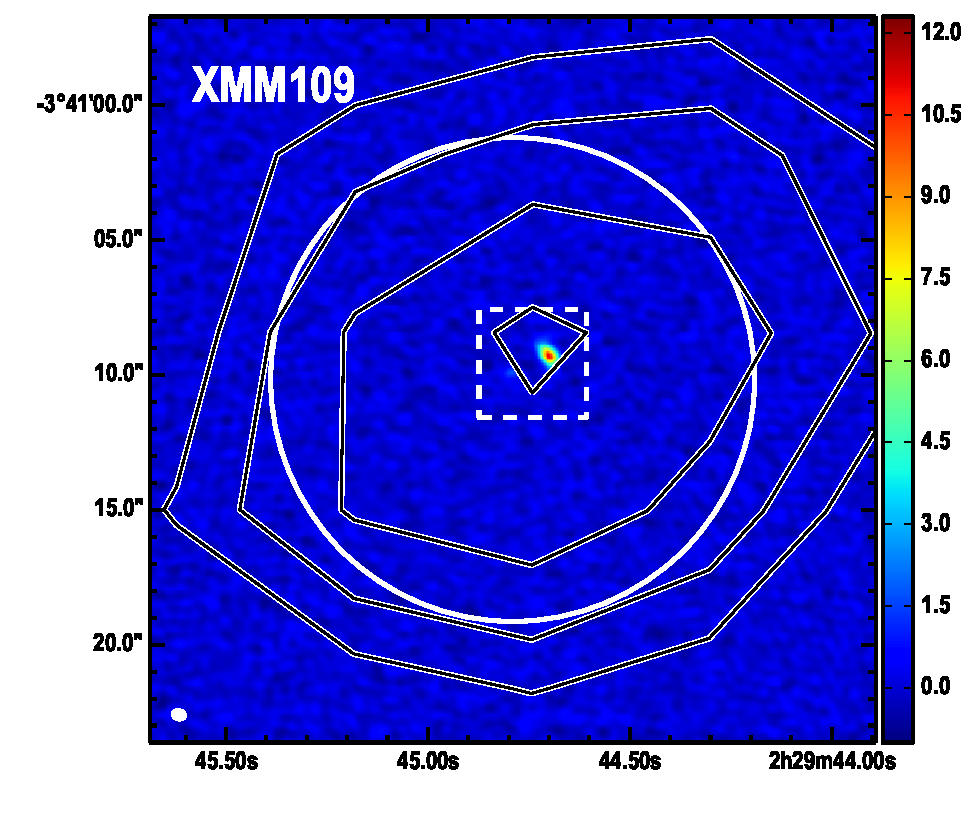
\includegraphics[width=0.245\textwidth]{overlays/XMM109_870_250.pdf}
%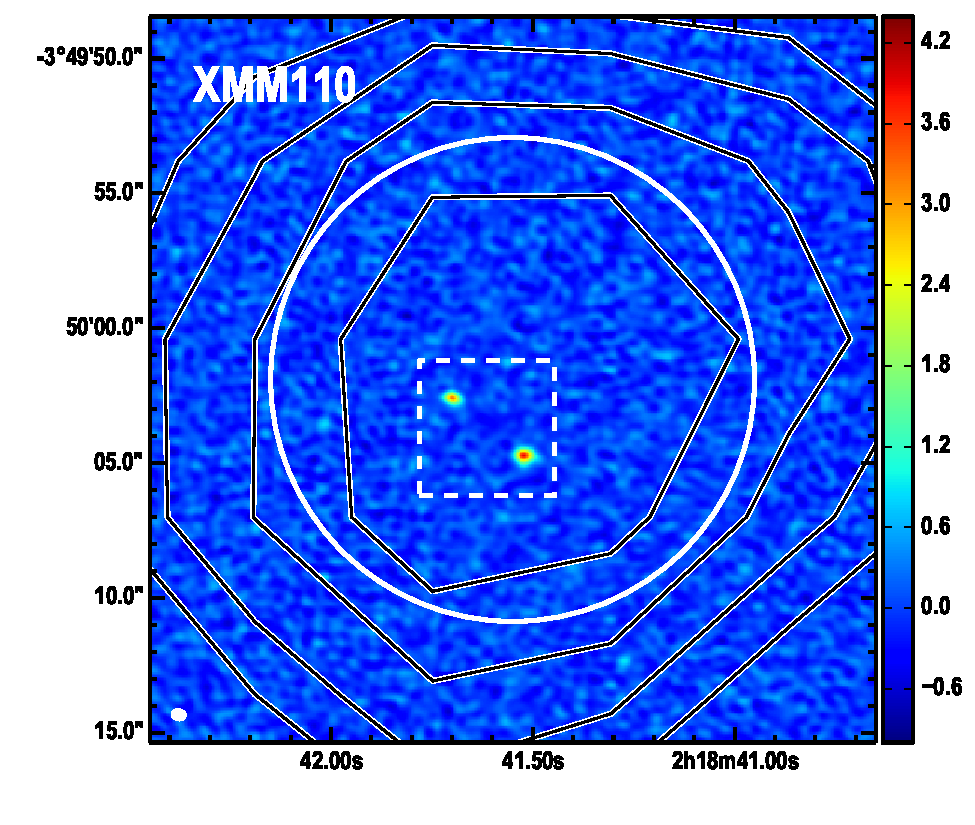
\includegraphics[width=0.245\textwidth]{overlays/XMM110_870_250.pdf}
%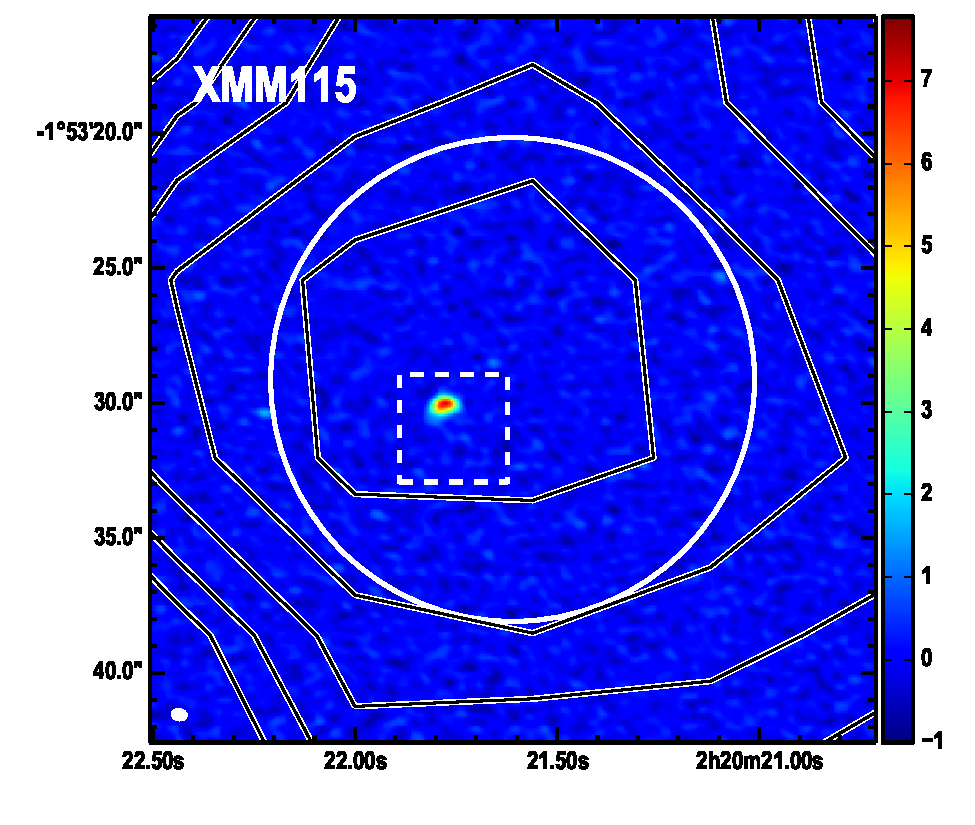
\includegraphics[width=0.245\textwidth]{overlays/XMM115_870_250.pdf}
%\end{centering}
%
%\caption{ Continued.}
%\addtocounter{figure}{-1}
%
%\end{figure*}

\begin{figure*}[!tbp] 
    \begin{centering}
%\epsscale{1.00} 
%\includegraphics[width=\textwidth]{cutouts_dec17.png}
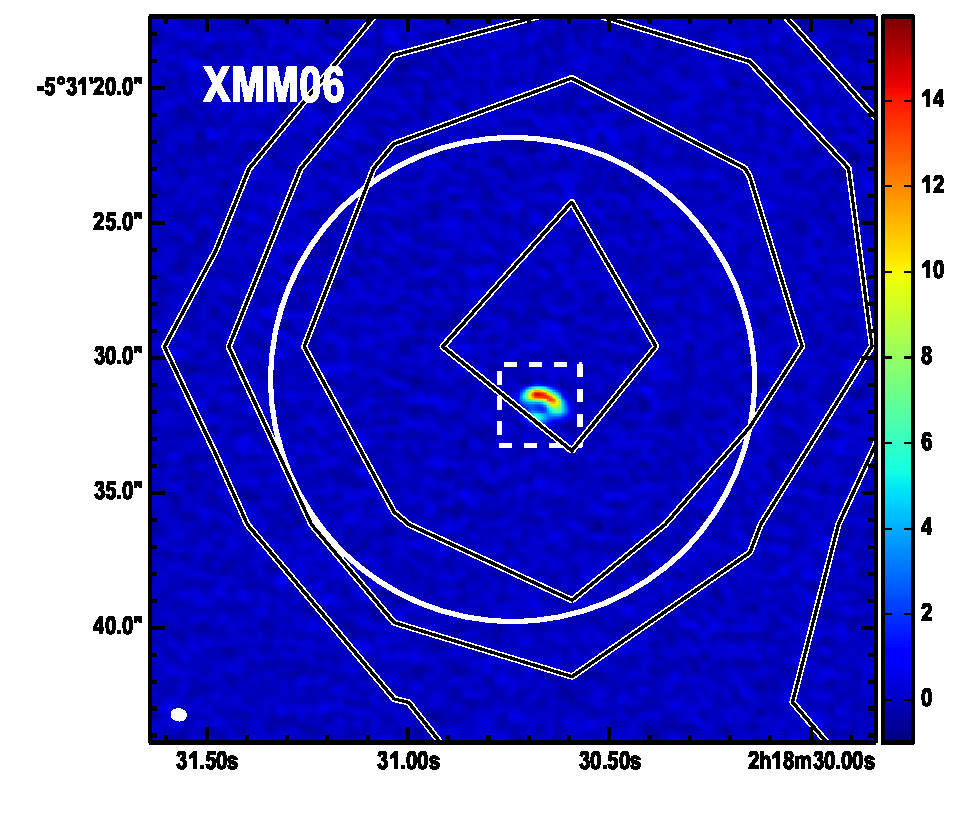
\includegraphics[width=0.245\textwidth]{overlays/XMM06_870_250.pdf}
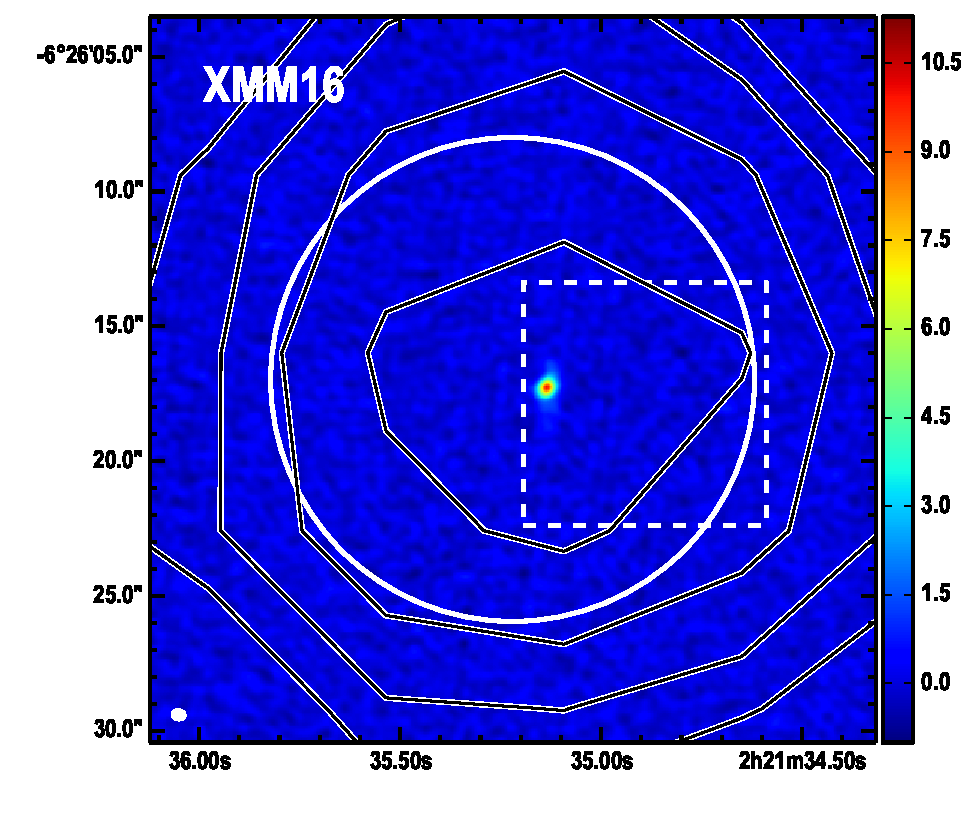
\includegraphics[width=0.245\textwidth]{overlays/XMM16_870_250.pdf}
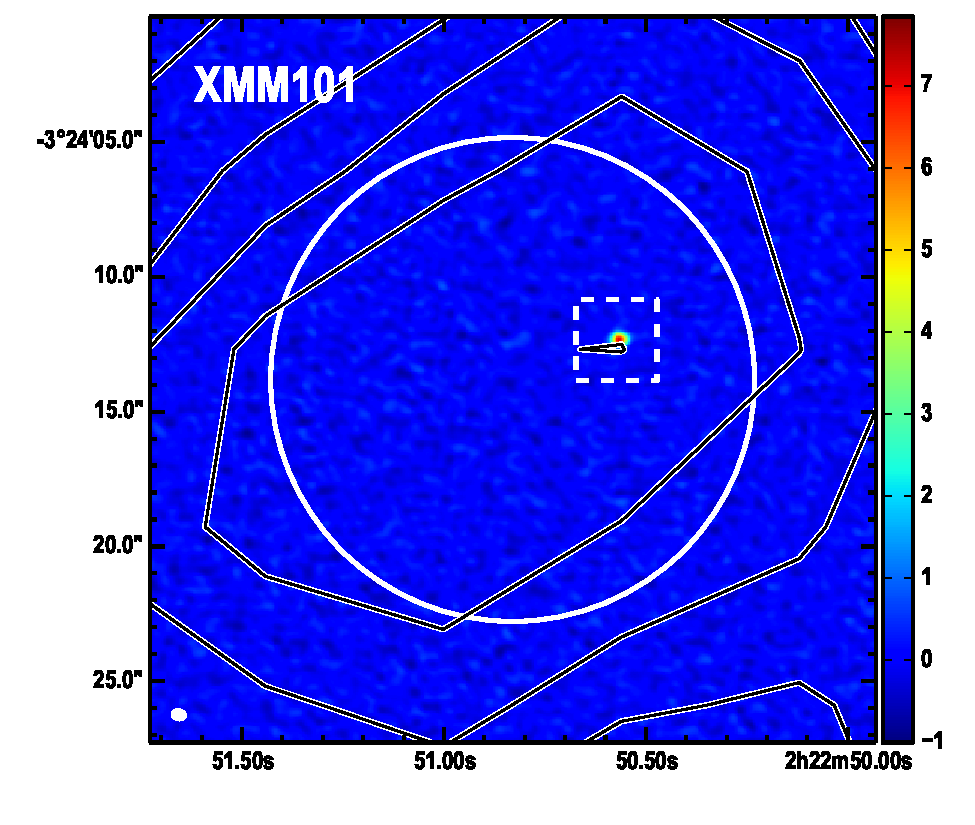
\includegraphics[width=0.245\textwidth]{overlays/XMM101_870_250.pdf}
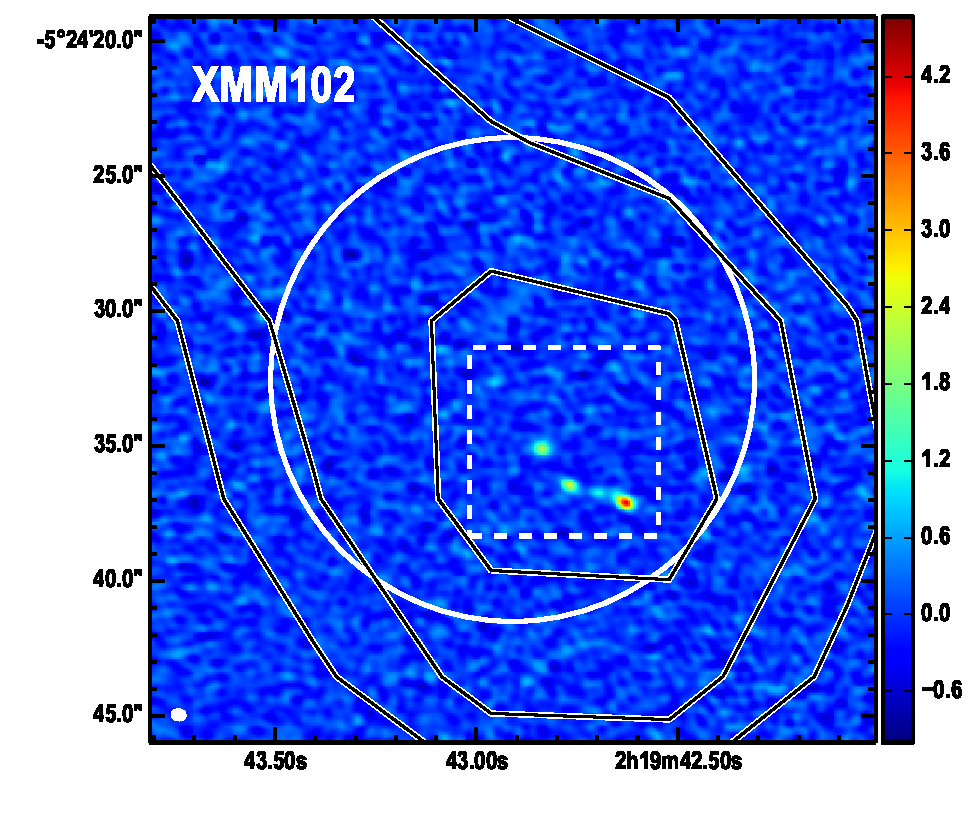
\includegraphics[width=0.245\textwidth]{overlays/XMM102_870_250.pdf}
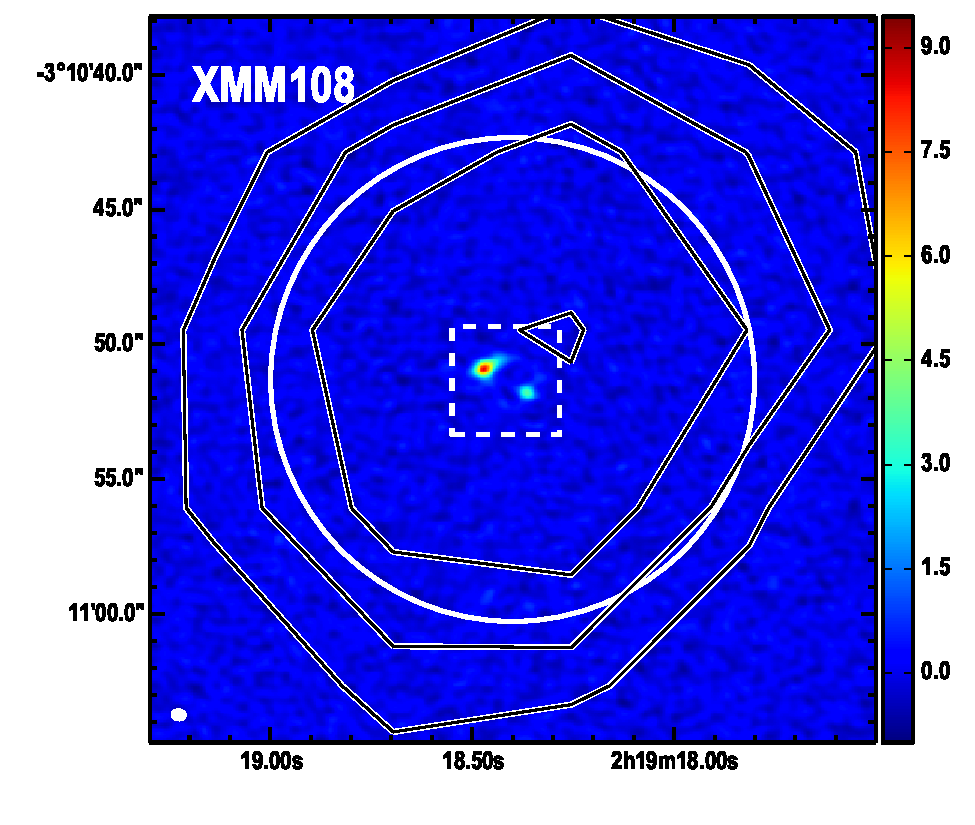
\includegraphics[width=0.245\textwidth]{overlays/XMM108_870_250.pdf}
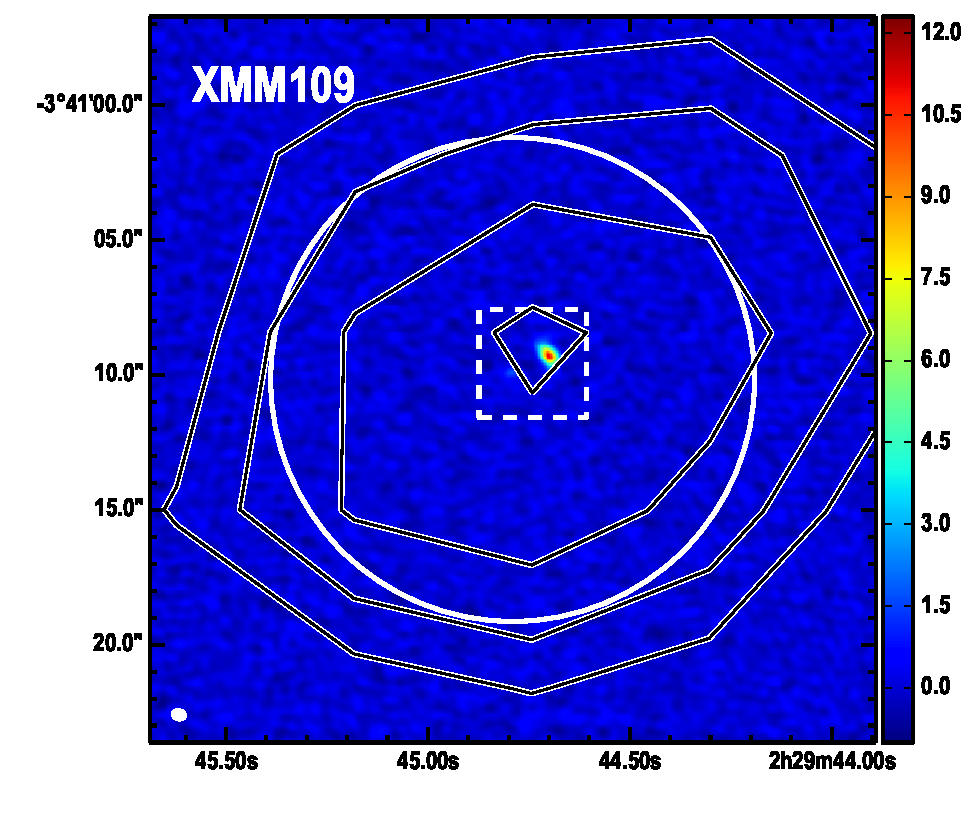
\includegraphics[width=0.245\textwidth]{overlays/XMM109_870_250.pdf}
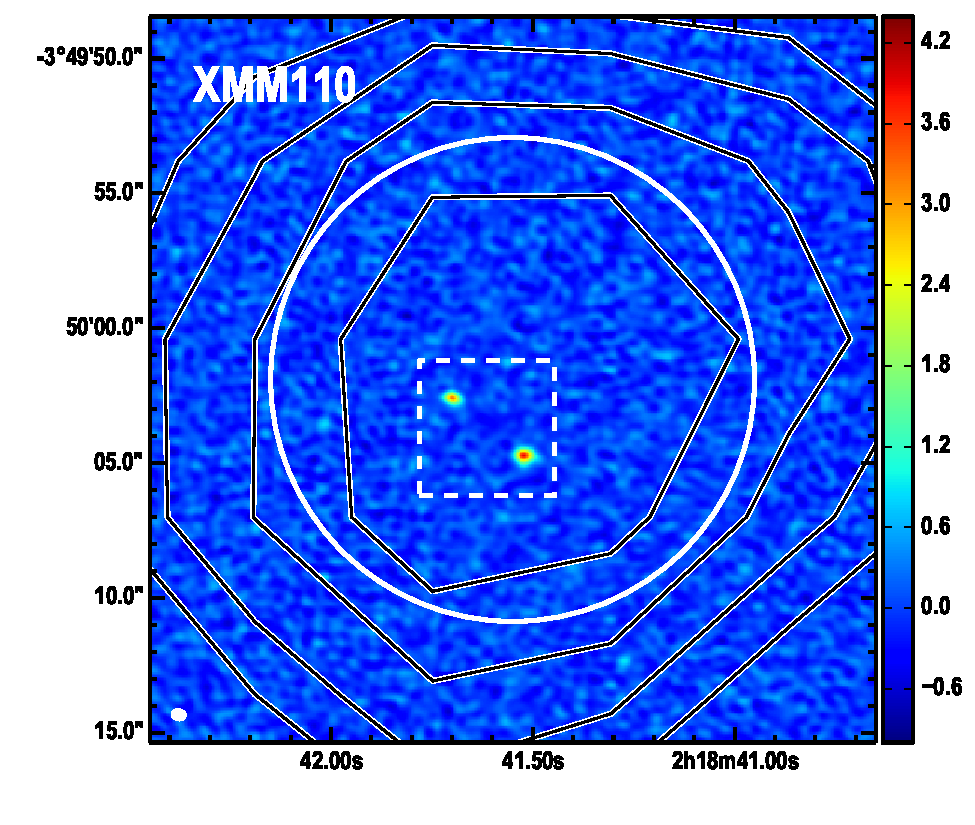
\includegraphics[width=0.245\textwidth]{overlays/XMM110_870_250.pdf}
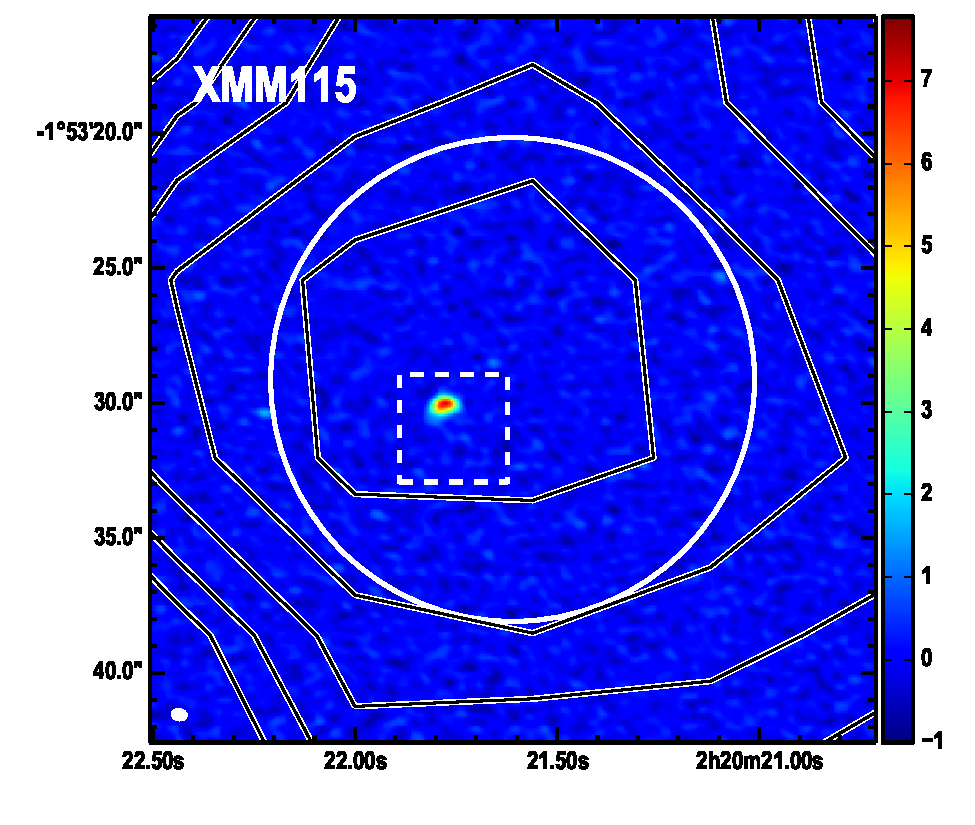
\includegraphics[width=0.245\textwidth]{overlays/XMM115_870_250.pdf}
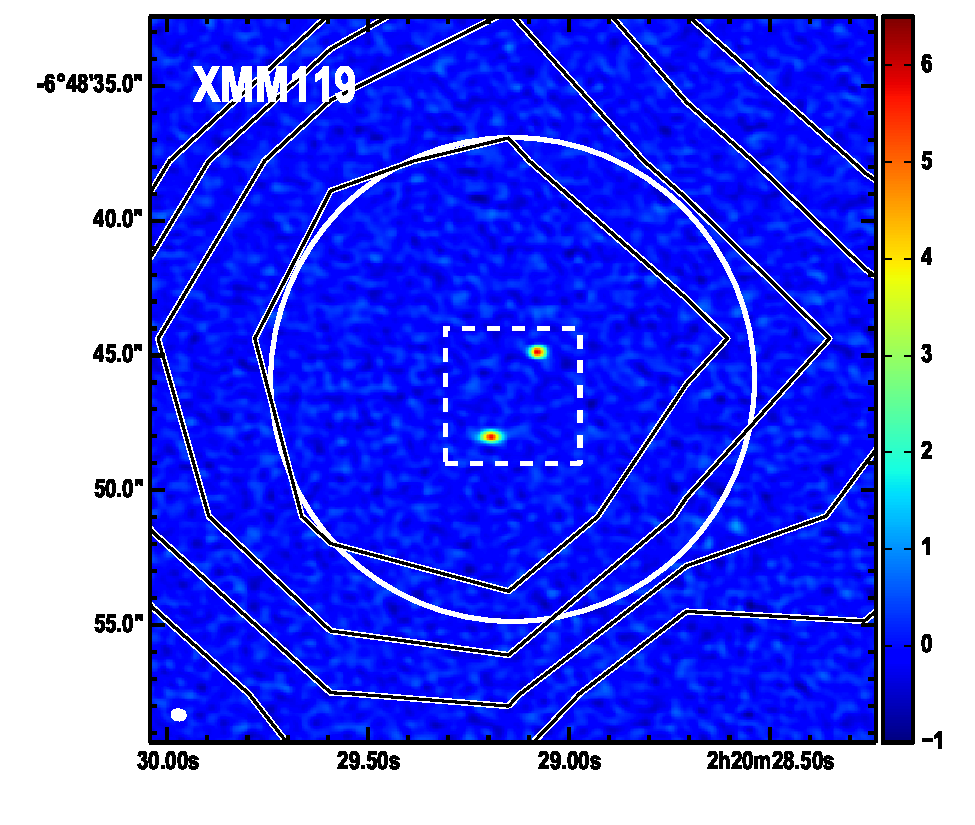
\includegraphics[width=0.245\textwidth]{overlays/XMM119_870_250.pdf}
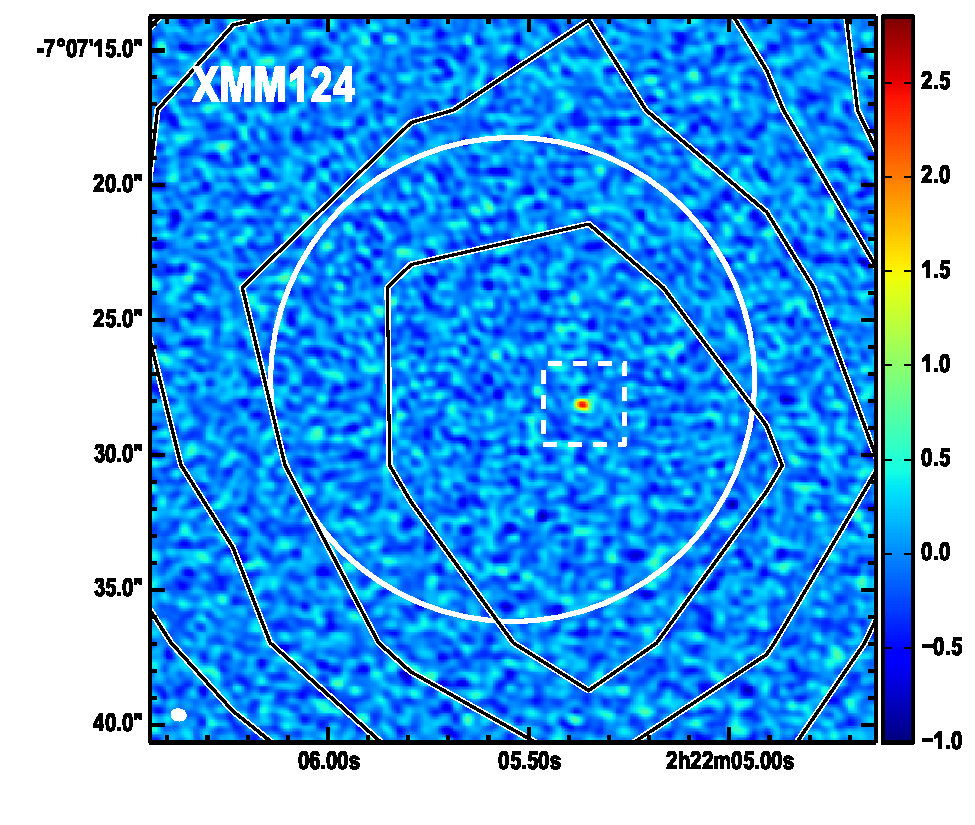
\includegraphics[width=0.245\textwidth]{overlays/XMM124_870_250.pdf}
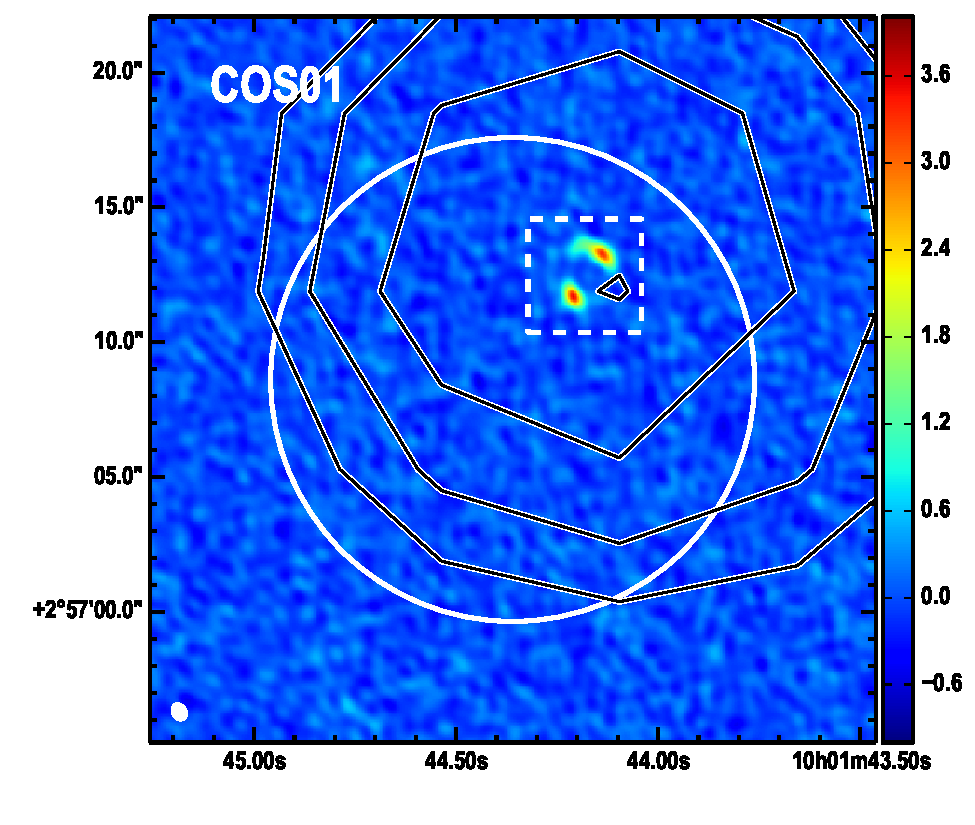
\includegraphics[width=0.245\textwidth]{overlays/COS01_870_250.pdf}
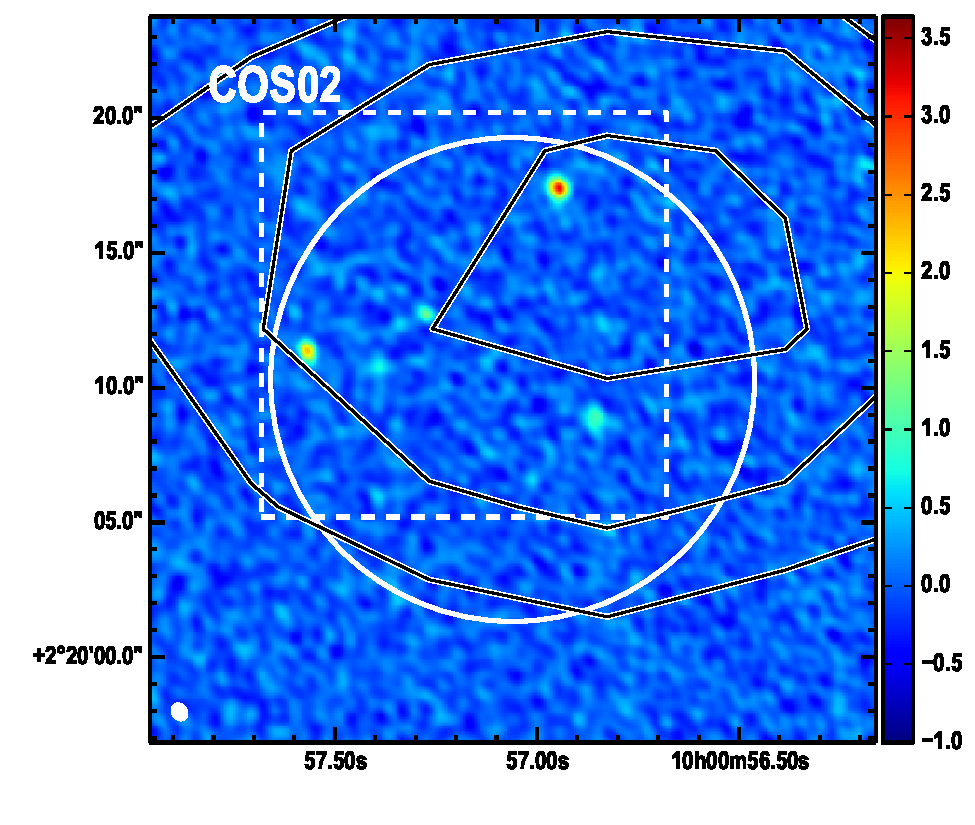
\includegraphics[width=0.245\textwidth]{overlays/COS02_870_250.pdf}
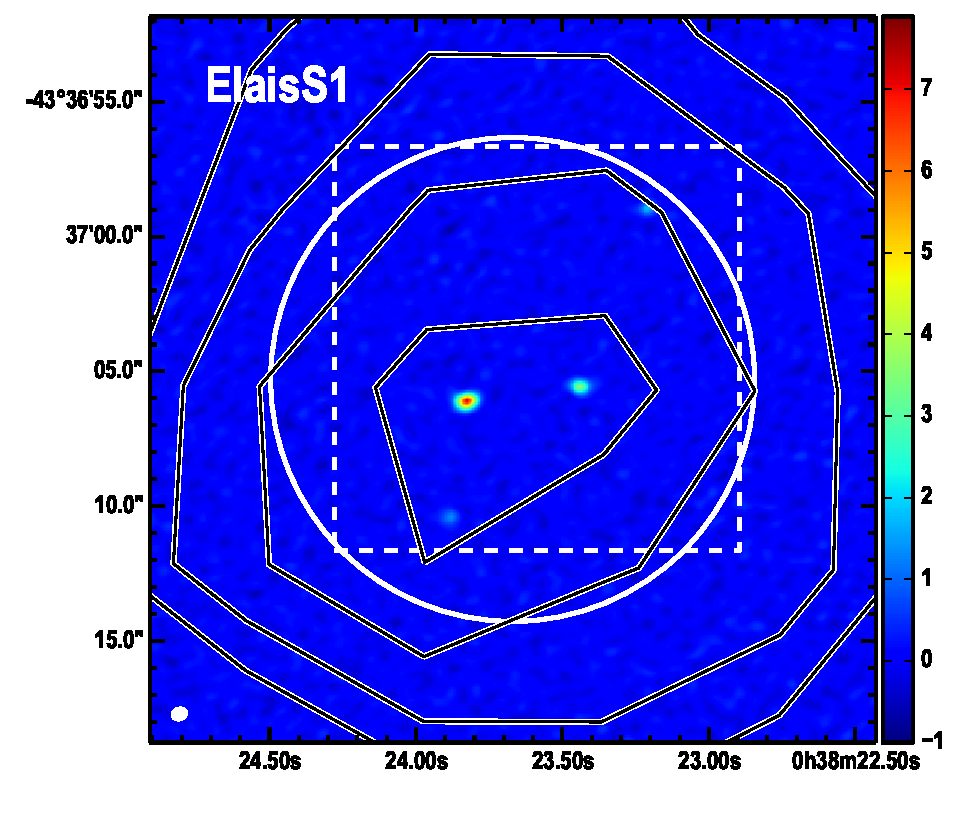
\includegraphics[width=0.245\textwidth]{overlays/ElaisS1_870_250.pdf}
\end{centering}

\caption{ Continued.}
%\addtocounter{figure}{-1}

\end{figure*}

In most targets, the peak of the SPIRE map is spatially coincident with the
location of the ALMA sources.  In one case where two ALMA sources are separated
by $\approx 10\arcsec$ (ADFS02), the elongation in the SPIRE 250$\,\mu$m map is
consistent with the angular separation of the two ALMA counterparts.
Otherwise, the SPIRE imaging is consistent with a single comoponent located at
the centroid of the ALMA sources.  This result is not a surprise, given the
typical angular separation of the ALMA sources ($\lesssim 5\arcsec$) and the
FWHM of the SPIRE beam at 250$\,\mu$m (18.1$\arcsec$). 

\subsection{Gemini-South Imaging}\label{sec:geminiobs}

Optical imaging observations using the Gemini Multi-Object Spectrograph-South
\citep[GMOS-S;][]{Hook:2004qy} were conducted in queue mode during the 2013B
semester as part of program GS-2013B-Q-77 (PI: R.~S.~Bussmann).  The goal of
the program is to use shallow $u$, $g$, $r$, $i$, and $z$ imaging to identify
structure at $z<1$ and determine which of the ALMA sources are affected by
gravitational lensing.  Some of the ALMA sources lie in regions with existing
deep optical imaging thanks to the extensive HerMES multi-wavelength dataset
--- these were excluded from our Gemini-S program.  The remaining targets are:
ADFS01, ADFS02, ADFS03, ADFS04, ADFS05, ADFS06, ADFS07, ADFS\_M0, ElaisS1,
XMM02, XMM05, XMM101, XMM108, XMM109, and XMM115.  Each of these targets were
observed for a total of 9$\,$minutes of on-source integration time in each of
$u$, $g$, $r$, $i$, and $z$.  The observations were obtained during dark time
in with adequate seeing conditions (image quality $ = 85\% \approx 1.1\arcsec$.

The data were reduced using the standard {\sc IRAF} Gemini GMOS reduction
routines, following the standard GMOS-S reduction steps in the example taken
from the Gemini observatory webpage
\footnote{http://www.gemini.edu/sciops/data-and-results/processing-software/getting-started\#gmos}.

We used the Sloan Digital Sky Survey (SDSS) or the 2 Micron All Sky Survey
(2MASS) to align the Gemini-S images to a common astrometric frame of
reference.  This imposes an rms uncertainty in the absolute astrometry of
$0\farcs2$ and $0\farcs4$ for SDSS and 2MASS, respectively.  The
astrometrically calibrated Gemini-S images served as the basis for aligning
higher resolution, smaller field-of-view imaging from {\it HST} or Keck that
were originally presented in \citet{Calanog:2014lr}.

%\begin{figure*}[!tbp] 
%%%\epsscale{1.00} 
%%%\includegraphics[width=\textwidth]{cutouts/cutouts_dec17.png}
%
%\caption{ Continued.
%\label{fig:imaging2}}
%
%\end{figure*}

%\input{table_opticalspectroscopy}

%\subsection{Ancillary Optical and Near-IR Imaging {\bf to be revised}}\label{sec:opticalimaging}

%In all cases where the SMA has clearly resolved multiple images of the
%background source, there is no evidence for submm emission from the lens.
%This means that detection of the foreground lens requires observations at
%optical or near-IR wavelengths.  This paper makes use of the best available
%optical or near-IR imaging to pinpoint the location of the lens and determine
%whether it comprises multiple galaxies.  This imaging is shown in grayscale in
%Figure~\ref{fig:imaging}, and the telescope and filter used are given in the
%lower left corner of each panel.  Fifteen objects use {\it HST} Snapshot
%imaging (marked as ``{\it HST} F110W'' in Figure~\ref{fig:imaging}), five use
%Keck-II/NIRC2-LGSAO imaging (marked as ``Keck-II\_NIRC2 Ks'' in
%Figure~\ref{fig:imaging}), five use full-orbit {\it HST} imaging (marked as
%``{\it HST} F160W'' in Figure~\ref{fig:imaging}), four use SDSS $i$-band
%imaging (marked as ``SDSS i'' in Figure~\ref{fig:imaging}), and two use WHT
%$K_{\rm s}$-band imaging (marked as ``WHT Ks'' in Figure~\ref{fig:imaging}).

%The focus of this paper is lens modeling of the SMA data.  A detailed analysis
%of the optical and near-IR imaging will appear in a set of papers specific to
%the {\it HST} Snapshot imaging (Amber et al., in prep.; Calanog et al. in
%prep.), the full-orbit {\it HST} imaging (Negrello et al., in prep., Dye et
%al., in prep.), and the Keck-II/NIRC2-LGSAO imaging (Calanog et al., in prep.)
%and the WHT $K_{\rm s}$ imaging (Mart/'/nez-Navajas et al., in prep.).

%To facilitate comparison with existing surveys for lenses based on SDSS
%spectroscopy \citep[e.g.,][]{Bolton:2008wd, Brownstein:2012rt}, we compute
%$i$-band photometry using SDSS Data Release 9 (DR9) for all of the objects in
%the SMA subsample.
%%Optical imaging of the candidate lenses is important for confirming their
%%existence, position on the sky, redshift (photometric), and for stellar
%%population synthesis analysis.  A detailed study of the stellar masses and
%%star-formation histories of the lensing galaxies is beyond the scope of this
%%paper, so the latter topic will be deferred to a subsequent publication.
%The imaging aspect of DR9 provides five optical bands: $u$, $g$, $r$, $i$, and
%$z$.  The 95\% completeness levels for point sources are $u=22.0$, $g=22.2$,
%$r=22.2$, $i=21.3$, and $z=20.5$ (AB mag), corresponding to flux densities of
%$5.7 \, \mu$Jy, $4.8 \, \mu$Jy, $4.8 \, \mu$Jy, $11.0 \, \mu$Jy, and $23.0 \,
%\mu$Jy, respectively.  The median seeing in the images at $r$-band is typically
%1$\farcs$3.

%We searched for counterparts in the DR9 catalog within a $2\arcsec$ radius of
%each expected lens position based on the best available optical or near-IR
%imaging.  If a counterpart was found, then it was assigned photometry directly
%from the DR9 catalog.  If no counterpart was found, we used our own custom
%aperture photometry code to measure the 2$\sigma$ limiting flux density at the
%position of the target (note that at these wavelengths, the lens is typically
%much brighter than the source).  We used a 4$\arcsec$ diameter circular aperture
%and computed the sky background in an annulus with an inner radius of
%2$\arcsec$ and an outer radius of 5$\arcsec$.  We measured the uncertainties by
%placing $N$ random apertures (where $N \approx 300$) of the same size and shape
%within 3$\arcmin$ of the lens candidate (taking care to avoid any objects found
%in the DR9 catalog) and computing the 68\% confidence interval of the
%dispersion in the measured flux densities.  The $i$-band AB magnitudes are
%reported in Table~\ref{tab:fluxes} (limits indicate 2$\sigma$ values), along
%with the {\it Herschel}/SPIRE and SMA 880$\, \mu$m measurements (the values
%reported in the table do not include absolute flux density calibration
%uncertainty of 7\%).

%To determine the aperture correction factor, we used the same
%technique to measure the flux densities of stars located within 3$\arcmin$ of
%the lens candidate with AB magnitudes between 15 and 22 and compared our values
%with those given in the SDSS DR9 catalog under the heading of ``modelMag\_{\it
%filter}''.  The aperture correction factor was typically 1.05-1.1.  



%\input{table_fluxes}

\section{Model Fits}\label{sec:modelfits}

\subsection{Model Fitting Methodology}\label{sec:modelfitsmeth}

An interferometer measures visibilities at discrete points in the {\it uv}
plane.  This is why pixel-to-pixel errors in the inverted and deconvolved
surface brightness map of an astronomical source are correlated.  The best way
to deal with this situation is to compare model and data visibilities rather
than surface brightness maps.  The methodology used in this paper is similar in
many aspects to that used in \citet{Bussmann:2012lr}, who presented the first
lens model derived from a visibility-plane analysis of interferometric imaging
of a strongly lensed DSFG discovered in wide-field submm surveys as well
\citet{Bussmann:2013lr}, who extended the work of \citet{Bussmann:2012lr} to a
statistically significant sample of 30 objects.  It also bears some resemblence
to the method used in \citet{Hezaveh:2013fk}, who undertake lens modeling of
interferometric data in the visibility plane.  We summarize important
information on the methodology here, taking care to highlight where any
differences occur between this work and that of our previous efforts.

We created and made publicly available custom software, called {\sc uvmcmcfit},
that is capable of modeling all of the ALMA sources in this paper efficiently
and reliably.  

Sources are assumed to be elliptical Gaussians that are parameterized by the
following six free parameters: the position of the source (relative to the
primary lens if a lens is present) ($\Delta \alpha_{\rm s}$ and $\Delta
\delta_{\rm s}$), the total intrinsic flux density ($S_{\rm in}$), the
effective radius intermediate axis length ($r_{\rm s} = \sqrt{a_{\rm s} b_{\rm
s}}$), the axial ratio ($q_{\rm s}$ =  $b_{\rm s}/a_{\rm s}$), and the position
angle ($\phi_{\rm s}$, degrees east of north).  The use of an elliptical
Gaussian represents a simplification from the S\'ersic profile
\citep{1968adga.book.....S}  that is justified based on the relatively weak
constraints on the S\'ersic index found in our previous work
\citep{Bussmann:2012lr, Bussmann:2013lr}.

When an intervening galaxy (or group of galaxies) is present along the line of
sight, {\sc uvmcmcfit} accounts for the deflection of light caused by this
structure using a simple ray-tracing routine that is adopted from a simple
Python routine written by A.~Bolton
\footnote{http://www.physics.utah.edu/$\sim$bolton/python\_lens\_demo/}.  This
represents a significant difference from \citet{Bussmann:2012lr} and
\citet{Bussmann:2013lr}, where we used the publicly available {\sc Gravlens}
software \citep{Keeton:2001lr} to map emission from the source plane to
the image plane for a given lensing mass distribution.  {\sc Gravlens} has a
wide range of lens mass profiles as well as a sophisticated algorithm for
mapping source-plane emission to the image-plane, but it also comes with a
significant input/output penalty that makes parallel computing prohibitively
expensive.  The use of pure-Python code for tracing the deflection of light
rays is a critical component of making {\sc uvmcmcfit} computationally
feasible.

In {\sc uvmcmcfit}, lens mass profiles are represented by $N_{\rm lens}$
singular isothermal ellipsoid (SIE) profiles, where $N_{\rm lens}$ is the
number of lensing galaxies found from the best available optical or near-IR
imaging \citep[a multitude of evidence supports the SIE as a reasonable choice;
for a recent review, see][]{Treu:2010fk}.  Each SIE is fully described by the
following five free parameters: the position of the lens relative to the
arbitrarily chosen ``image center'' based on the ALMA 870$\,\mu$m emission and
any lensing galaxies seen in the optical or near-IR ($\Delta \alpha_{\rm lens}$
and $\Delta \delta_{\rm lens}$; these can be compared with the position of the
optical or near-IR counterpart relative to the ``image center'': $\Delta
\alpha_{\rm NIR}$ and $\Delta \delta_{\rm NIR}$), the mass of the lens
(parameterized in terms of the intermediate axis angular Einstein radius,
$\theta_{\rm E}$), the axial ratio of the lens ($q_{\rm lens} = b_{\rm lens} /
a_{\rm lens}$), and the position angle of the lens ($\phi_{\rm lens}$; degrees
east of north).  Unless otherwise stated, when optical or near-IR imaging
suggests the presence of additional lenses (see Figure~\ref{fig:uvmodels}), we
estimate centroids for each lens by-eye and fix the positions of the additional
lenses with respect to the primary lens.  Each additional lens thus has 3 free
parameters: $\theta_{\rm E}$, $q_{\rm lens}$, and $\phi_{\rm lens}$.  We assume
secondary, tertiary, etc., lenses are located at the same redshift as the
primary lens.  

The total number of free parameters for any given system is $N_{\rm free} = 5 +
3 \times (N_{\rm lens} - 1) + 6 * N_{\rm source}$, where $N_{\rm source}$ is
the number of S\'ersic profiles used.

We use uniform priors for all model parameters.  The prior on the position of
the lenses covers $\pm0\farcs6$ ($1\farcs0$) in both RA and Dec, a value that
reflects the 1-$\sigma$ absolute astrometric solution between the ALMA and
optical/near-IR images of $0\farcs2$ ($0\farcs4$) for SDSS-based (2MASS-based)
astrometric calibration.  In section~\ref{sec:objectbyobject}, we discuss the
level of agreement between the astrometry from the images and the astrometry
from the lens modeling on an object-by-object basis.  For $\theta_{\rm E}$, the
prior covers $0\farcs1 - 6\arcsec$.  The axial ratios of the lenses and sources
are restricted to be $q_{\rm lens} > 0.3$ and $q_{\rm s} > 0.2$. No prior is
placed on the position angle of the lens or source.  The intrinsic flux density
for any source is allowed to vary from 0.1$\,$mJy to the total flux density
observed by the ALMA.  The source position is allowed to vary over any
reasonable range necessary to fit the data (typically, this is $\pm
1-2\arcsec$).  The effective radius is allowed to vary from $0\farcs01 -
1\farcs5$.

The surface brightness map generated as part of {\sc uvmcmcfit} is then
converted to a ``simulated visibility'' dataset ($V_{\rm model}$) in much the
same way as MIRIAD's {\sc uvmodel} routine.  Indeed, the code used in {\sc
uvmcmcfit} is a direct Python port of {\sc uvmodel} (the use of {\sc uvmodel}
itself is not possible for the same reason as {\sc Gravlens}: constant
input/output makes parallel computing prohibitively expensive).  {\sc
uvmcmcfit} computes the Fourier transform of the surface brightness map and
samples the resulting visibilities in a way that closely matches the sampling
of the actual observed ALMA visibility dataset ($V_{\rm ALMA}$).

The quality of fit for a given set of model parameters is determined from the
maximum likelihood estimate $MLE$ according to the following equation:

\begin{equation}
    MLE = \sum_{u, v} \frac{|V_{\rm ALMA} - V_{\rm
    model}|^2}{\sigma^2} + log(2 \pi \sigma^2) 
\end{equation}

%\begin{equation}
%    MLE = -\frac{1}{2} (MLE_{\rm real} + MLE_{\rm imag}),
%\end{equation}

%\begin{equation}
%    MLE_{\rm real} = \sum_{u, v} \frac{[Re(V_{\rm ALMA}) - Re(V_{\rm
%    model})]^2}{\sigma^2} + log(2 \pi \sigma^2), 
%\end{equation}

%\begin{equation}
%    MLE_{\rm imag} = \sum_{u, v} \frac{[Im(V_{\rm ALMA}) - Im(V_{\rm
%    model})]^2}{\sigma^2} + log(2 \pi \sigma^2),
%\end{equation}

\noindent where $\sigma$ is the 1$\sigma$ uncertainty level for each
visibility and is determined from the scatter in the visibilities within a
single spectral window (this is a natural weighting scheme).  

We use {\sc emcee} \citep{Foreman-Mackey:2013yq} to sample the posterior
probability density function (PDF) of our model parameters.  {\sc emcee} is a
Markov chain Monte Carlo (MCMC) code that uses an affine-invariant ensemble
sampler to obtain significant performance advantages over standard MCMC
sampling methods \citep{goodmanweare}.  

We employ a ``burn-in'' phase with 512 walkers and 500-1000 iterations (i.e.,
$\approx 250,000-500,000$ samplings of the posterior PDF) to identify the
best-fit model parameters.  This position then serves as the basis to
initialize the ``final'' phase with 512 walkers and 10 iterations (i.e., 5,120
samplings of the posterior PDF) to determine uncertainties on the best-fit
model parameters.  
%The autocorrelation time for each parameter in a given ensemble of walkers and
%is of order unity for each parameter, implying that we have 5,000 independent
%samplings of the posterior PDF, more than enough to obtain a robust
%measurement of the mean and uncertainty on each parameter of the model.

During each MCMC iteration, we also measure the magnification factor at
870$\,\mu$m, $\mu_{870}$, for each source.  This is done simply by taking the
ratio of the total flux density in the lensed image of the model ($S_{\rm out}$
to the total flux density in the unlensed, intrinsic source model ($S_{\rm
in}$).  The use of an aperture when computing $\mu_{870}$ is important when
source profiles are used with significant flux at large radii (e.g., some types
of S\'ersic profiles).  For an elliptical Gaussian, such a step is unneccessary
(note that we did test this and found only $\approx 10\%$ difference between
$\mu_{870}$ computed with and without an aperture.  The best-fit value and
1$\sigma$ uncertainty on $\mu_{870}$ are drawn from the posterior PDF, as with
the other parameters of the model.

\subsection{Individual Model Fits}\label{objectbyobject}

In this section, we present our model fits and describe each source in detail.

{\bf ADFS01:} Three sources are detected by ALMA, each of which is weakly
lensed by a bright foreground galaxy seen in the {\it HST} image.  Alternative
scenarios involving strong lensing can be ruled out by the location of the
lens: $\approx 2-3\arcsec$ north of the centroid of the ALMA sources (the rms
error in the astrometry is set from 2MASS at a level of $\approx 0\farcs5$) as
well as the unusual location and fluxes of the ALMA sources relative to each
other.  We assume an Einstein radius of $0\farcs5$ and fix the position angle
of the lens to be between 40-50 degrees to match the orientation seen in the
{\it HST} image.  Larger Einstein radii can be ruled out by the absence of
counter images north of the lens.

{\bf ADFS02:} Two sources are detected by ALMA, both of which are weakly lensed
by a foreground galaxy in the {\it HST} image.  The ALMA sources have the
largest separation of any in our sample overall: $\approx 10\arcsec$.  We
assume an Einstein radius of $1\farcs5$ for the foreground lens as a ``maximal
lensing'' scenario.  This results in magnification factors of $\mu_{870} = 2.3
\pm 0.1$ and $\mu_{870} = 1.2 \pm 0.1$ for the two sources.  Our constraints on
the true Einstein radius of the lens are weak, so these values for $\mu_{870}$
should be regarded as upper limits.

{\bf ADFS03:} Three sources are detected by ALMA, none of which appear to be
lensed (the closest bright {\it HST} source is located $\approx 13\arcsec$ away
from the ALMA sources).

{\bf ADFS04:} Three sources are detected by ALMA.  In this paper, we have
assumed that all three are unlensed.  There is a group of three sources
detected in our Gemini-S optical imaging located $\approx 7\arcsec$ east of the
ALMA sources.  This distance is so large that plausible mass ranges for the
Gemini-S sources would imply at most a factor of 1.1-1.2 boost in the apparent
flux densities of the ALMA sources.

{\bf ADFS05:} Two sources are detected by ALMA.  The nearest possible lens is
located $\approx 8\arcsec$ from the ALMA sources, indicating that lensing is
likely to be irrelevant in this system.  The two ALMA sources are similarly
bright ($S_{870} = 8.27 \pm 0.53\,$mJy and $S_{870} = 9.07 \pm 0.27\,$mJy) and
separated by $\approx 0\farcs8$, corresponding to a projected physical distance
of $\approx 6\,$kpc. This distance is typical of the pericentric passage
distance in hydrodynamical simulations of major mergers
\citep[e.g.,][]{Hayward:2012lr}.  A plausible scenario is that ADFS05
represents a major merger that just experienced a first pass which
significantly enhanced star-formation in both sources.

{\bf ADFS06:} Three sources are detected by ALMA, all of which are weakly
lensed by a foreground galaxy seen in the {\it HST} image.  We assume an
Einstein radius of $0\farcs5$ for the lens, as values larger than this produce
multiple images of the ALMA sources.  Based on the brightness of the lens, we
consider to be unlikely values for the Einstein radius that are smaller than
$0\farcs5$, so the results we report for this object should be robust.

{\bf ADFS07:} This is a single source that is strongly lensed by a foreground
galaxy seen in the {\it HST} image.  The lensed source is not detected by {\it
HST}.  The source is highly elongated ($q_s = 0.31 \pm 0.01$), but fits the
data very well.  The position of the lens according to the lens model is
consistent with the position in the {\it HST} image given the $0\farcs5$
fundamental uncertainty due to using the 2MASS system as the fundamental basis
for the astrometry.

{\bf ADFS\_M0:} Two sources are detected by ALMA, both of which are weakly
lensed by a group of small galaxies detected in the {\it HST} image.  We
represent the gravitational potential of the group with a single SIE lens and
an Einstein radius of $1\farcs0$.  Values larger than this produce additional
counter images that are not seen in the ALMA imaging.  We cannot rule out
smaller Einstein radii, but we consider these unlikely given the number of
sources and their brightness in the {\it HST} image.

{\bf CDFS\_M0:} This is a complex, very well constrained system.  Two sources
are detected by ALMA: one is strongly lensed and the other is weakly lensed.
In addition, the lens is detected by ALMA (this is one of two sources in the
entire ALMA sample that is unresolved by ALMA).  These facts work together to
provide very tight constraints on the system.  Since the lens is detected by
ALMA, its position relative to the lensed images is unambiguous.  Also, because
there is a strongly lensed source with multiple images, the Einstein radius of
the lens is unambiguous.  A byproduct of these two facts is that the
magnification factor of the weakly lensed source is known to very high
precision as well.  It experiences a magnification factor of $\mu_{870} =
1.520\pm0.002$ despite being located $\approx4\arcsec$ north of the lens (which
has an Einstein radius of $1.353\pm0.005$).  We use these numbers to inform our
estimates of the Einstein radius for weakly lensed sources without the
excellent contraints provided by this system.

{\bf CDFS\_M1:} Two sources are detected by ALMA, both of which are weakly
lensed by a foreground galaxy seen in the {\it HST} image.  There is also a
3$\sigma$ peak coincident with {\it HST} source that may be an indication that
the lens has been detected by ALMA.  We do not attempt to model this 3$\sigma$
peak.  We assume an Einstein radius of $0\farcs5$ for the lens, since larger
values predict the existence of counter images that are not seen by ALMA.  The
second ALMA source is located $\approx5\arcsec$ from the lens but still
experiences a significant magnification of $\mu_{870} = 1.12 \pm 0.02$.

{\bf ECDFS02:} This system is very similar to ADFS05, except that here the two
ALMA sources are separated by $\approx 0\farcs4$ rather than $0\farcs8$ and one
source is brighter than the other by a factor of 2.  Assuming the two sources
have similar mass to light ratios, their brightness ratios indicate major
merger rather than minor merger activity.  The projected physical distance is
$\approx 2-3$kpc, assuming a redshift of $z=2$ for the ALMA sources.  This
could be an example of a major merger approaching final coalescence and
experiencing a significant boost in star-formation due to enhancements in the
local gas density brought about by dynamical friction forces during the merger.

{\bf ElaisS1:} Four sources are detected by ALMA, all of which are weakly
lensed by a foreground galaxy seen in the {\it HST} image.  We assume an
Einstein radius of $1\farcs5$ for the lens as larger values begin to predict
counter images that are not seen by ALMA.  The magnification factors reported
here should be regarded as upper limits since we do not have strong constraints
on the lower limit of the Einstein radius of the lens (e.g., the magnication
factor for the source that is directly south of the lens is reported here to
have $\mu_{870} = 1.68 \pm 0.06$, but values as small as 1.1-1.2 are likely
plausible as well).

{\bf COS01:} This system is similar to ADFS07: a single source that is strongly
lensed by a foreground galaxy seen in the {\it HST} image.  In fact, the
background source is also detected by {\it HST} as well as Keck/NIRC-II
adaptive optics imaging, and a lens model has been published based on these
data \citep{Calanog:2014lr}.  The morphology of the lensed emission is very
different between the Keck and ALMA imaging, suggesting differential
magnification is important in this object.  The very small sizes of the sources
are consistent with this as well ($r_s = 0.023 \pm 0.003\arcsec$, Keck and $r_s
= 0.055 \pm 0.007\arcsec$, ALMA).  Adopting a redshift of $z=2$ for the lensed
source implies physical sizes of $\approx 150\,$pc and $\approx 300\,$pc for
the rest-frame optical and rest-frame far-IR, respectively.

{\bf COS02:} Five sources are detected by ALMA, none of which appear to be
lensed.  This is one of two objects in our sample that have five ALMA
counterparts.  There are also a number of $2-3\sigma$ peaks in the map that
could be real, further increasing the multiplicity rate for this object.
However, there are also negative peaks of somewhat similar amplitude at a
relatively high rate in this map, so we choose to be conservative in our
assessment of what is a real source for this object.  Some of the ALMA sources
have counterparts detected in the {\it HST} image.

{\bf XMM01:} Three sources are detected by ALMA, all of which are weakly lensed
by two foreground galaxies seen in the {\it HST} and Keck/NIRC-II imaging.  The
ALMA imaging is broadly consistent with SMA data originally presented in
\citet{Fu:2013lr}, with two bright sources and a much fainter third source very
close to the more southern bright source.  We assume Einstein radii of
$0\farcs5$ for both lenses to reproduce the approach used in \citet{Fu:2013lr}.
This results in magnification factors for the three sources of $\mu_{879}
\approx 1.6 - 1.7$, similar to \citet{Fu:2013lr}.

{\bf XMM02:} Two sources are detected by ALMA, both of which are weakly lensed.
This system is similar to ADFS02, although the two ALMA sources are much closer
and the lens must be less massive in order to avoid producing multiple images
of the closest ALMA source.  The fainter ALMA source has a much lower
magnification factor than the brighter source ($\mu_{870} = 1.10 \pm 0.01$ vs.
$\mu_{870} = 1.63 \pm 0.11$).  As with ADFS02, we caution that these
magnification factors represent the ``maximal lensing'' scenario and hence
should be considered upper limits.

{\bf XMM03:} One source is detected by ALMA, and it is weakly lensed by two
foreground galaxies seen in the {\it HST} images.  We assume an Einstein radius
of 1$\arcsec$ for the foreground lenses and fix the positions of both lenses
according to the location of the foreground galaxies in the {\it HST} image.
As with XMM02, this is the ``maximal lensing'' scenario, so our magnification
measurement of $\mu_{870} = 1.80 \pm 0.16$ should be considered an upper limit.

{\bf XMM04:} Two sources are detected by ALMA, none of which appear to be
lensed.  The brighter ALMA source is weakly detected in the CFHT $i$-band
image.  

{\bf XMM05:} One source is detected by ALMA, and it is weakly lensed by a group
of foreground galaxies seen in the {\it HST} image.  We assume an Einstein
radius of $0\farcs2$ for the nearest lensing galaxy and allow a $\pm0\farcs4$
shift in its position relative to that indicated by the {\it HST} image (which
has its astrometry tied to SDSS).  We represent the remaining members of the
group as a single SIS located $4\farcs5$ south and $4\farcs5$ east of the image
centroid and having an Einstein radius of $2\farcs0$.  This is meant to
represent the ``maximal lensing'' scenario, so our measurement of $\mu_{870}$
should be regarded as an upper limit.  The presence of two $3\sigma$ peaks
located near the center of the residual image indicates that the model does not
fit the data perfectly.  This could be an indication that either of our
assumptions for the lens potential or source structure are oversimplifications.
Higher resolution imaging is needed to determine the most likely cause.

{\bf XMM06:} One source is detected by ALMA, and it is strongly lensed by one
foreground galaxy seen in the {\it HST} image.  The lensed source is not
detected in the {\it HST} image.  This object also has high quality SMA imaging
and an accompanying lens model that produces consistent results with those
given here \citep{Bussmann:2013lr}.

{\bf XMM16:} Three sources are detected by ALMA, all of which are weakly lensed
by a foreground galaxy detected in the {\it HST} image and located $\approx
6\arcsec$ from the ALMA sources.  The central source is much brighter than the
other two sources, which makes fitting a model challenging.  We forced the
positions of the second and third sources to be at least $0\farcs5$ and
$-0\farcs5$ away from the first source in declination, respectively.
Furthermore, we fixed the position of the lens to be located $2\farcs5$ west
and $0\farcs5$ south of the image centroid given in Table~\ref{tab:position}.
We also fixed the Einstein radius to be $1\farcs0$, a typical value for
isolated galaxies in this sample and in \citet{Bussmann:2013lr}.  Because the
source is so far from the lens, the magnification factor is only $\mu_{870} =
1.19 \pm 0.01$.

{\bf XMM101:} One source is detected by ALMA, and it appears to be unlensed.  A
faint smudge seen in the {\it HST} image of this source is due to a star
located $3\farcs5$ northeast of the ALMA source.

{\bf XMM102:} Five sources are detected by ALMA, none of which appear to be
lensed.  There are a few faint smudges seen in the {\it HST} image which are
likely to be the rest-frame optical counterparts to the ALMA sources.  The ALMA
sources are all arranged in a chain like shape, possibly suggestive of a larger
filamentary overdensity in which they might reside.

{\bf XMM108:} One source is detected by ALMA, and it is strongly lensed by one
foreground galaxy detected in the Gemini-S image.  There is a $\approx
0\farcs5$ offset in the position of the foreground galaxy between the lens
model and the Gemini-S image.  Given the absolute astrometric uncertainty of
$0\farcs2$ (based on SDSS), we do not consider this offset to be significant.
The presence of a handful of $\pm3\sigma$ peaks in the residual map is likely
an indication that our assumption of a single Gaussian to describe the source
morphology is an oversimplification.

{\bf XMM109:} One source is detected by ALMA, and it is strongly lensed by one
foreground galaxy detected in the Gemini-S image.  As with XMM108, there is a
$\approx 0\farcs5$ offset between the lens position according to the lens model
and the Gemini-S image.  We do not consider this offset significant.  An
alternative model in which the lens is sub-mm luminous cannot be ruled out, but
we consider this unlikely for a number of reasons.  First, it is a more complex
model (having two sources and one lens, rather than one source and one lens).
Second, lenses are very rarely detected in sub-mm imaging.  Third, the shape
and location of the ALMA sources relative to the Gemini-S source are typical of
strongly lensed objects (consistent with the very low residuals).  Fourth, the
alternative lens model predicts the lensed source to have an intrinsic flux
density of $\approx 13 \,$mJy, which would make it the brightest source in the
sample.

{\bf XMM110:} Two sources are detected by ALMA, neither of which are lensed.
The faint, diffuse emission seen in the CFHT $i$-band image is atypical of
lensing galaxies.  The nearest bright galaxy seen at $i$-band is located
$\approx 18\arcsec$ southeast of the ALMA sources.

{\bf XMM115:} One source is detected by ALMA, and it is weakly lensed by a
foreground galaxy seen in the {\it HST} image.  We assume an Einstein radius of
$0\farcs5$ to represent the ``maximal lensing'' scenario.  Due to the
elliptical nature of the lens, this results in a magnification factor of
$\mu_{870} = 3.72 \pm 0.42$.  The {\it HST} morphology is complex: diffuse
emission to the north of the lens could be a detection of the background source
or could be a long spiral arm associated with the lensing galaxy.

{\bf XMM119:} Two sources are detected by ALMA, both of which are weakly
lensed by a foreground galaxy detected in the {\it HST} image.  An Einstein
radius of $1\farcs5$ is used to represent the ``maximal lensing'' scenario and
results in magnification factors of $\mu_{870} = 2.25 \pm 0.17$ and $\mu_{870}
= 1.48 \pm 0.09$.

{\bf XMM124:} One source is detected by ALMA, and it is coincident (within the
astrometric uncertainty) with a late-type galaxy seen in the {\it HST} image.
Here, we assume that the {\it HST} source is the true counterpart to the ALMA
source, implying that no lensing is occuring.  

\begin{figure*}[!tbp] 
    \begin{centering}
%\epsscale{1.00} 
%\includegraphics[width=\textwidth]{cutouts_dec17.png}
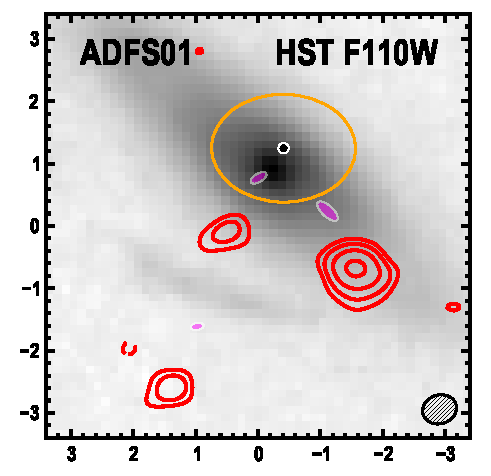
\includegraphics[width=0.162\textwidth]{modelfit/ADFS01_optical_bestfit.pdf}
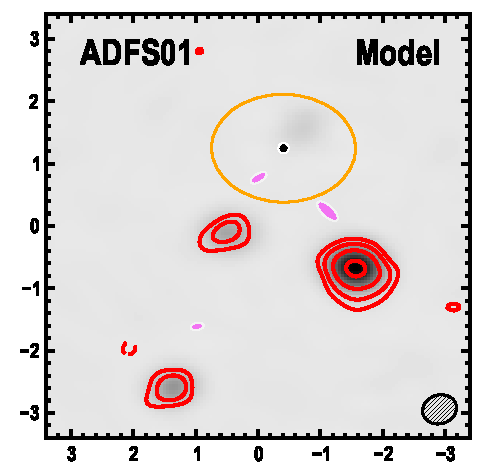
\includegraphics[width=0.162\textwidth]{modelfit/ADFS01_model_bestfit.pdf}
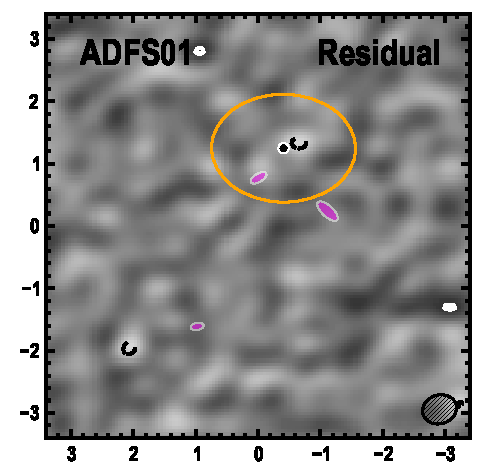
\includegraphics[width=0.162\textwidth]{modelfit/ADFS01_residual_bestfit.pdf}
\includegraphics[width=0.162\textwidth]{modelfit/ADFS02_optical_bestfit.pdf}
\includegraphics[width=0.162\textwidth]{modelfit/ADFS02_model_bestfit.pdf}
\includegraphics[width=0.162\textwidth]{modelfit/ADFS02_residual_bestfit.pdf}
\includegraphics[width=0.162\textwidth]{modelfit/ADFS03_optical_bestfit.pdf}
\includegraphics[width=0.162\textwidth]{modelfit/ADFS03_model_bestfit.pdf}
\includegraphics[width=0.162\textwidth]{modelfit/ADFS03_residual_bestfit.pdf}
\includegraphics[width=0.162\textwidth]{modelfit/ADFS04_optical_bestfit.pdf}
\includegraphics[width=0.162\textwidth]{modelfit/ADFS04_model_bestfit.pdf}
\includegraphics[width=0.162\textwidth]{modelfit/ADFS04_residual_bestfit.pdf}
\includegraphics[width=0.162\textwidth]{modelfit/ADFS05_optical_bestfit.pdf}
\includegraphics[width=0.162\textwidth]{modelfit/ADFS05_model_bestfit.pdf}
\includegraphics[width=0.162\textwidth]{modelfit/ADFS05_residual_bestfit.pdf}
\includegraphics[width=0.162\textwidth]{modelfit/ADFS06_optical_bestfit.pdf}
\includegraphics[width=0.162\textwidth]{modelfit/ADFS06_model_bestfit.pdf}
\includegraphics[width=0.162\textwidth]{modelfit/ADFS06_residual_bestfit.pdf}
\includegraphics[width=0.162\textwidth]{modelfit/ADFS07_optical_bestfit.pdf}
\includegraphics[width=0.162\textwidth]{modelfit/ADFS07_model_bestfit.pdf}
\includegraphics[width=0.162\textwidth]{modelfit/ADFS07_residual_bestfit.pdf}
\includegraphics[width=0.162\textwidth]{modelfit/ADFS_M0_optical_bestfit.pdf}
\includegraphics[width=0.162\textwidth]{modelfit/ADFS_M0_model_bestfit.pdf}
\includegraphics[width=0.162\textwidth]{modelfit/ADFS_M0_residual_bestfit.pdf}
\includegraphics[width=0.162\textwidth]{modelfit/CDFS_M0_optical_bestfit.pdf}
\includegraphics[width=0.162\textwidth]{modelfit/CDFS_M0_model_bestfit.pdf}
\includegraphics[width=0.162\textwidth]{modelfit/CDFS_M0_residual_bestfit.pdf}
\includegraphics[width=0.162\textwidth]{modelfit/CDFS_M1_optical_bestfit.pdf}
\includegraphics[width=0.162\textwidth]{modelfit/CDFS_M1_model_bestfit.pdf}
\includegraphics[width=0.162\textwidth]{modelfit/CDFS_M1_residual_bestfit.pdf}
\includegraphics[width=0.162\textwidth]{modelfit/ECDFS02_optical_bestfit.pdf}
\includegraphics[width=0.162\textwidth]{modelfit/ECDFS02_model_bestfit.pdf}
\includegraphics[width=0.162\textwidth]{modelfit/ECDFS02_residual_bestfit.pdf}
\includegraphics[width=0.162\textwidth]{modelfit/ElaisS1_optical_bestfit.pdf}
\includegraphics[width=0.162\textwidth]{modelfit/ElaisS1_model_bestfit.pdf}
\includegraphics[width=0.162\textwidth]{modelfit/ElaisS1_residual_bestfit.pdf}
\includegraphics[width=0.162\textwidth]{modelfit/COS01_optical_bestfit.pdf}
\includegraphics[width=0.162\textwidth]{modelfit/COS01_model_bestfit.pdf}
\includegraphics[width=0.162\textwidth]{modelfit/COS01_residual_bestfit.pdf}
\includegraphics[width=0.162\textwidth]{modelfit/COS02_optical_bestfit.pdf}
\includegraphics[width=0.162\textwidth]{modelfit/COS02_model_bestfit.pdf}
\includegraphics[width=0.162\textwidth]{modelfit/COS02_residual_bestfit.pdf}
\end{centering}

\caption{ Model fits for each target in the ALMA sample, 3 panels per target.
{\it Left}: ALMA 870$\mu$m imaging (red contours, starting at $\pm 3\sigma$ and
increasing by factors of 2) overlaid on best available optical or near-IR
imaging (grayscale, with telescope and filter printed in upper right corner).
The location and morphology of all sources used in the model are represented by
magenta ellipses.  If a lens is present, its location is given by a black
circle and its critical curve is traced by an orange line.  The FWHM size of
the ALMA synthesized beam is shown in the lower left corner of each panel.
{\it Middle}: Same as {\it left}, but showing best-fit model in grayscale.
{\it Right}: Same as {\it left}, but showing resdiual image obtained from
subtracting best-fit model from the data.  \label{fig:uvmodels}}
\addtocounter{figure}{-1}

\end{figure*}

%\begin{figure*}[!tbp] 
%    \begin{centering}
%%\epsscale{1.00} 
%%\includegraphics[width=\textwidth]{cutouts_dec17.png}
%\end{centering}
%
%\caption{ Continued.}
%\addtocounter{figure}{-1}
%
%\end{figure*}
%
%\begin{figure*}[!tbp] 
%    \begin{centering}
%%\epsscale{1.00} 
%%\includegraphics[width=\textwidth]{cutouts_dec17.png}
%\includegraphics[width=0.162\textwidth]{modelfit/CDFS_M0_optical_bestfit.pdf}
%\includegraphics[width=0.162\textwidth]{modelfit/CDFS_M0_model_bestfit.pdf}
%\includegraphics[width=0.162\textwidth]{modelfit/CDFS_M0_residual_bestfit.pdf}
%\includegraphics[width=0.162\textwidth]{modelfit/CDFS_M1_optical_bestfit.pdf}
%\includegraphics[width=0.162\textwidth]{modelfit/CDFS_M1_model_bestfit.pdf}
%\includegraphics[width=0.162\textwidth]{modelfit/CDFS_M1_residual_bestfit.pdf}
%\includegraphics[width=0.162\textwidth]{modelfit/ECDFS02_optical_bestfit.pdf}
%\includegraphics[width=0.162\textwidth]{modelfit/ECDFS02_model_bestfit.pdf}
%\includegraphics[width=0.162\textwidth]{modelfit/ECDFS02_residual_bestfit.pdf}
%\includegraphics[width=0.162\textwidth]{modelfit/ElaisS1_optical_bestfit.pdf}
%\includegraphics[width=0.162\textwidth]{modelfit/ElaisS1_model_bestfit.pdf}
%\includegraphics[width=0.162\textwidth]{modelfit/ElaisS1_residual_bestfit.pdf}
%\end{centering}
%
%\caption{ Continued.}
%\addtocounter{figure}{-1}
%
%\end{figure*}

\begin{figure*}[!tbp] 
    \begin{centering}
%\epsscale{1.00} 
%\includegraphics[width=\textwidth]{cutouts_dec17.png}
\includegraphics[width=0.162\textwidth]{modelfit/XMM01_optical_bestfit.pdf}
\includegraphics[width=0.162\textwidth]{modelfit/XMM01_model_bestfit.pdf}
\includegraphics[width=0.162\textwidth]{modelfit/XMM01_residual_bestfit.pdf}
\includegraphics[width=0.162\textwidth]{modelfit/XMM02_optical_bestfit.pdf}
\includegraphics[width=0.162\textwidth]{modelfit/XMM02_model_bestfit.pdf}
\includegraphics[width=0.162\textwidth]{modelfit/XMM02_residual_bestfit.pdf}
\includegraphics[width=0.162\textwidth]{modelfit/XMM03_optical_bestfit.pdf}
\includegraphics[width=0.162\textwidth]{modelfit/XMM03_model_bestfit.pdf}
\includegraphics[width=0.162\textwidth]{modelfit/XMM03_residual_bestfit.pdf}
\includegraphics[width=0.162\textwidth]{modelfit/XMM04_optical_bestfit.pdf}
\includegraphics[width=0.162\textwidth]{modelfit/XMM04_model_bestfit.pdf}
\includegraphics[width=0.162\textwidth]{modelfit/XMM04_residual_bestfit.pdf}
\includegraphics[width=0.162\textwidth]{modelfit/XMM05_optical_bestfit.pdf}
\includegraphics[width=0.162\textwidth]{modelfit/XMM05_model_bestfit.pdf}
\includegraphics[width=0.162\textwidth]{modelfit/XMM05_residual_bestfit.pdf}
\includegraphics[width=0.162\textwidth]{modelfit/XMM06_optical_bestfit.pdf}
\includegraphics[width=0.162\textwidth]{modelfit/XMM06_model_bestfit.pdf}
\includegraphics[width=0.162\textwidth]{modelfit/XMM06_residual_bestfit.pdf}
\includegraphics[width=0.162\textwidth]{modelfit/XMM16_optical_bestfit.pdf}
\includegraphics[width=0.162\textwidth]{modelfit/XMM16_model_bestfit.pdf}
\includegraphics[width=0.162\textwidth]{modelfit/XMM16_residual_bestfit.pdf}
\includegraphics[width=0.162\textwidth]{modelfit/XMM101_optical_bestfit.pdf}
\includegraphics[width=0.162\textwidth]{modelfit/XMM101_model_bestfit.pdf}
\includegraphics[width=0.162\textwidth]{modelfit/XMM101_residual_bestfit.pdf}
\includegraphics[width=0.162\textwidth]{modelfit/XMM102_optical_bestfit.pdf}
\includegraphics[width=0.162\textwidth]{modelfit/XMM102_model_bestfit.pdf}
\includegraphics[width=0.162\textwidth]{modelfit/XMM102_residual_bestfit.pdf}
\includegraphics[width=0.162\textwidth]{modelfit/XMM108_optical_bestfit.pdf}
\includegraphics[width=0.162\textwidth]{modelfit/XMM108_model_bestfit.pdf}
\includegraphics[width=0.162\textwidth]{modelfit/XMM108_residual_bestfit.pdf}
\includegraphics[width=0.162\textwidth]{modelfit/XMM109_optical_bestfit.pdf}
\includegraphics[width=0.162\textwidth]{modelfit/XMM109_model_bestfit.pdf}
\includegraphics[width=0.162\textwidth]{modelfit/XMM109_residual_bestfit.pdf}
\includegraphics[width=0.162\textwidth]{modelfit/XMM110_optical_bestfit.pdf}
\includegraphics[width=0.162\textwidth]{modelfit/XMM110_model_bestfit.pdf}
\includegraphics[width=0.162\textwidth]{modelfit/XMM110_residual_bestfit.pdf}
\includegraphics[width=0.162\textwidth]{modelfit/XMM115_optical_bestfit.pdf}
\includegraphics[width=0.162\textwidth]{modelfit/XMM115_model_bestfit.pdf}
\includegraphics[width=0.162\textwidth]{modelfit/XMM115_residual_bestfit.pdf}
\includegraphics[width=0.162\textwidth]{modelfit/XMM119_optical_bestfit.pdf}
\includegraphics[width=0.162\textwidth]{modelfit/XMM119_model_bestfit.pdf}
\includegraphics[width=0.162\textwidth]{modelfit/XMM119_residual_bestfit.pdf}
\includegraphics[width=0.162\textwidth]{modelfit/XMM124_optical_bestfit.pdf}
\includegraphics[width=0.162\textwidth]{modelfit/XMM124_model_bestfit.pdf}
\includegraphics[width=0.162\textwidth]{modelfit/XMM124_residual_bestfit.pdf}
\end{centering}

\caption{ Continued.}
\addtocounter{figure}{-1}

\end{figure*}

\clearpage
\LongTables
\begin{deluxetable*}{lcccccccc}[!tbp]
%\rotate
%\resizebox{\textwidth}{!}{%
\tabletypesize{\scriptsize}
\tablecolumns{9}
%\tablewidth{7.5in}
\tablecaption{Lens properties from parameters of model fits to ALMA sources. Parameters without uncertainties were fixed to the given value. }
\tablehead{
\colhead{} & 
\colhead{} & 
\colhead{RA$_{870}$} &
\colhead{Dec$_{870}$} &
\colhead{$\sigma_{\rm RA}$} &
\colhead{$\sigma_{\rm Dec}$} &
\colhead{$\theta_{\rm E}$} &
\colhead{} &
\colhead{$\phi_{\rm lens}$}
\\
\colhead{Short name} & 
\colhead{Lens ID} & 
\colhead{(J2000)} &
\colhead{(J2000)} &
\colhead{($\arcsec$)} &
\colhead{($\arcsec$)} &
\colhead{($\arcsec$)} &
\colhead{$q_{\rm lens}$} &
\colhead{(deg)}
}
\startdata
ADFS01   & Lens0  & 04:50:57.688 & $-$53:16:53.10 & 0.005 & 0.06 & $1.0          $ & $0.707\pm0.141$ & $ 93\pm  7$  \\
ADFS02   & Lens0  & 04:50:27.213 & $-$52:41:27.73 & 0.004 & 0.06 & $1.5          $ & $0.897\pm0.047$ & $ 74\pm 18$  \\
ADFS06   & Lens0  & 04:33:40.413 & $-$54:03:39.39 & 0.009 & 0.07 & $0.5          $ & $0.662\pm0.135$ & $ 37\pm 12$  \\
ADFS07   & Lens0  & 04:41:53.867 & $-$54:03:53.23 & 0.001 & 0.01 & $1.006\pm0.004$ & $0.794\pm0.008$ & $ 99\pm  1$  \\
ADFS\_M0 & Lens0  & 04:38:30.910 & $-$54:18:29.11 & 0.003 & 0.12 & $1.0          $ & $0.723\pm0.068$ & $ 82\pm  9$  \\
CDFS\_M0 & Lens0  & 03:27:52.025 & $-$29:09:12.15 & 0.001 & 0.01 & $1.354\pm0.006$ & $0.955\pm0.007$ & $ 80\pm  6$  \\
CDFS\_M1 & Lens0  & 03:32:10.907 & $-$27:05:32.09 & 0.002 & 0.01 & $0.5          $ & $0.807\pm0.006$ & $176\pm  3$  \\
COS01    & Lens0  & 10:01:44.174 & $+$02:57:12.75 & 0.001 & 0.02 & $0.956\pm0.005$ & $0.775\pm0.025$ & $ 72\pm  1$  \\
ElaisS1  & Lens0  & 00:38:23.481 & $-$43:37:01.90 & 0.013 & 0.19 & $1.5          $ & $0.790\pm0.067$ & $ 44\pm  6$  \\
XMM01    & Lens0  & 02:20:16.746 & $-$06:01:42.58 &  ---  & ---  & $0.5          $ & $0.801\pm0.062$ & $ 48\pm 14$  \\
 ---     & Lens1  & 02:20:16.423 & $-$06:01:42.18 &  ---  & ---  & $0.5          $ & $0.882\pm0.072$ & $ 90\pm 17$  \\
XMM02    & Lens0  & 02:22:01.671 & $-$03:33:38.45 & 0.008 & 0.10 & $0.5          $ & $0.706\pm0.124$ & $ 67\pm 11$  \\
XMM03    & Lens0  & 02:25:48.129 & $-$04:17:52.20 &  ---  & ---  & $1.0          $ & $0.531\pm0.180$ & $ 45\pm 14$  \\
 ---     & Lens1  & 02:25:47.815 & $-$04:17:48.30 &  ---  & ---  & $1.0          $ & $0.569\pm0.197$ & $ 67\pm 16$  \\
XMM05    & Lens0  & 02:30:05.947 & $-$03:41:53.35 & 0.005 & 0.06 & $0.519\pm0.044$ & $0.852\pm0.097$ & $ 24\pm 20$  \\
XMM06    & Lens0  & 02:18:30.673 & $-$05:31:31.99 & 0.001 & 0.01 & $0.507\pm0.004$ & $0.596\pm0.009$ & $157\pm  1$  \\
XMM108   & Lens0  & 02:19:18.398 & $-$03:10:51.31 & 0.002 & 0.13 & $0.928\pm0.007$ & $0.902\pm0.024$ & $ 26\pm  7$  \\
XMM109   & Lens0  & 02:29:44.738 & $-$03:41:09.52 & 0.002 & 0.01 & $0.743\pm0.008$ & $0.703\pm0.050$ & $ 26\pm  1$  \\
XMM115   & Lens0  & 02:20:21.768 & $-$01:53:30.88 & 0.002 & 0.03 & $0.5          $ & $0.547\pm0.050$ & $ 11\pm  6$  \\
XMM119   & Lens0  & 02:20:29.234 & $-$06:48:46.30 & 0.005 & 0.05 & $1.0          $ & $0.663\pm0.094$ & $ 64\pm  6$  \\
\enddata
\label{tab:intrinsic}
%\tnt{a}{Multiple lens redshifts have been measured for these targets.  The redshift uncertainty is 0.001 in all cases.}
%\tablenotetext{c}{WHT/ACAM?}
%\tablenotetext{d}{\citet{Bussmann:2012lr}}
% 
%\tablenotetext{a}{\citet{Lupu:2012ly}}
%\tablenotetext{b}{\citet{Harris:2012fr}}
%\tablenotetext{c}{\citet{2011ApJ...726L..22F}}
%\tablenotetext{d}{Riechers et al., in prep.}
%\tablenotetext{e}{Krips et al., in prep.}
%\tablenotetext{f}{\citet{Cox:2011fk}}
%\tablenotetext{g}{George et al., in prep.}
%%\tablenotetext{h}{\citep{Wardlow:2013lr}}
\end{deluxetable*}

\clearpage
\LongTables
\begin{deluxetable*}{llccccccc}[!tbp]
%\rotate
%\resizebox{\textwidth}{!}{%
\tabletypesize{\scriptsize}
\tablecolumns{9}
%\tablewidth{7.5in}
\tablecaption{Intrinsic properties from parameters of model fits to ALMA sources.
Uncertainties in flux densities do not include absolute calibration uncertainty
of $\approx 10\%$.}
\tablehead{
\colhead{} & 
\colhead{} & 
\colhead{$\Delta$RA$_{870}$} &
\colhead{$\Delta$Dec$_{870}$} &
\colhead{$S_{870}$} &
\colhead{$r_{\rm s}$} &
\colhead{} &
\colhead{$\phi_{\rm s}$} & 
\colhead{}
\\
\colhead{Short name} & 
\colhead{Source ID} & 
\colhead{(J2000)} &
\colhead{(J2000)} &
\colhead{(mJy)} &
\colhead{($\arcsec$)} &
\colhead{$q_{\rm s}$} &
\colhead{(deg)} &
\colhead{$\mu_{870}$}
}
\startdata
ADFS01 & Source0   & $-0.734\pm0.069$ & $-1.070\pm0.053$ & $ 4.32\pm 0.28$ & $0.112\pm0.006$ & $ 0.41\pm 0.05$ & $ 45\pm  3$ & $ 1.64\pm 0.10$ \\
ADFS01 & Source1   & $ 1.415\pm0.056$ & $-2.912\pm0.059$ & $ 1.49\pm 0.11$ & $0.059\pm0.018$ & $ 0.54\pm 0.12$ & $ 94\pm 48$ & $ 1.26\pm 0.03$ \\
ADFS01 & Source2   & $ 0.427\pm0.055$ & $-0.514\pm0.059$ & $ 0.83\pm 0.13$ & $0.084\pm0.020$ & $ 0.50\pm 0.13$ & $125\pm 14$ & $ 2.72\pm 0.33$ \\
ADFS02 & Source0   & $-0.868\pm0.050$ & $ 0.938\pm0.048$ & $ 2.54\pm 0.18$ & $0.055\pm0.010$ & $ 0.83\pm 0.09$ & $131\pm 20$ & $ 2.29\pm 0.13$ \\
ADFS02 & Source1   & $ 7.496\pm0.058$ & $ 2.190\pm0.059$ & $ 3.72\pm 0.20$ & $0.179\pm0.012$ & $ 0.59\pm 0.08$ & $ 63\pm  6$ & $ 1.20\pm 0.01$ \\
ADFS03 & Source0   & $ 2.343\pm0.007$ & $ 3.284\pm0.005$ & $ 7.50\pm 0.24$ & $0.109\pm0.008$ & $ 0.70\pm 0.11$ & $ 92\pm 14$ & $ 1.00\pm 0.00$ \\
ADFS03 & Source1   & $-2.191\pm0.013$ & $-3.320\pm0.011$ & $ 3.84\pm 0.27$ & $0.099\pm0.019$ & $ 0.53\pm 0.17$ & $135\pm 24$ & $ 1.00\pm 0.00$ \\
ADFS03 & Source2   & $-2.503\pm0.035$ & $ 0.886\pm0.019$ & $ 2.06\pm 0.30$ & $0.122\pm0.040$ & $ 0.51\pm 0.17$ & $ 89\pm 20$ & $ 1.00\pm 0.00$ \\
ADFS04 & Source0   & $-1.126\pm0.005$ & $-0.319\pm0.004$ & $ 8.65\pm 0.23$ & $0.073\pm0.010$ & $ 0.67\pm 0.15$ & $133\pm 24$ & $ 1.00\pm 0.00$ \\
ADFS04 & Source1   & $ 0.876\pm0.011$ & $ 0.908\pm0.009$ & $ 3.53\pm 0.18$ & $0.048\pm0.019$ & $ 0.71\pm 0.19$ & $ 84\pm 43$ & $ 1.00\pm 0.00$ \\
ADFS04 & Source2   & $-0.437\pm0.017$ & $-1.088\pm0.016$ & $ 2.76\pm 0.16$ & $0.093\pm0.020$ & $ 0.58\pm 0.20$ & $131\pm 38$ & $ 1.00\pm 0.00$ \\
ADFS05 & Source0   & $ 0.067\pm0.008$ & $ 0.588\pm0.015$ & $ 7.02\pm 0.42$ & $0.136\pm0.012$ & $ 0.38\pm 0.06$ & $ 23\pm  5$ & $ 1.00\pm 0.00$ \\
ADFS05 & Source1   & $-0.060\pm0.009$ & $-0.268\pm0.018$ & $ 8.27\pm 0.53$ & $0.193\pm0.015$ & $ 0.42\pm 0.06$ & $ 17\pm  4$ & $ 1.00\pm 0.00$ \\
ADFS06 & Source0   & $ 0.333\pm0.101$ & $-0.513\pm0.040$ & $ 5.14\pm 0.39$ & $0.091\pm0.006$ & $ 0.39\pm 0.05$ & $142\pm  4$ & $ 1.70\pm 0.14$ \\
ADFS06 & Source1   & $ 0.865\pm0.123$ & $-0.420\pm0.041$ & $ 4.09\pm 0.29$ & $0.165\pm0.013$ & $ 0.43\pm 0.06$ & $141\pm  4$ & $ 1.42\pm 0.07$ \\
ADFS06 & Source2   & $ 0.604\pm0.108$ & $ 0.739\pm0.077$ & $ 1.56\pm 0.20$ & $0.077\pm0.015$ & $ 0.75\pm 0.16$ & $101\pm 40$ & $ 1.79\pm 0.18$ \\
ADFS07 & Source0   & $ 0.131\pm0.005$ & $-0.105\pm0.006$ & $ 3.28\pm 0.13$ & $0.128\pm0.005$ & $ 0.30\pm 0.01$ & $ 24\pm  1$ & $ 9.81\pm 0.31$ \\
ADFS\_M0 & Source0 & $-1.340\pm0.043$ & $-1.816\pm0.119$ & $ 9.81\pm 0.33$ & $0.225\pm0.006$ & $ 0.46\pm 0.02$ & $178\pm  1$ & $ 1.43\pm 0.03$ \\
ADFS\_M0 & Source1 & $ 0.658\pm0.039$ & $ 1.569\pm0.111$ & $ 4.27\pm 0.24$ & $0.180\pm0.010$ & $ 0.25\pm 0.02$ & $167\pm  2$ & $ 1.52\pm 0.07$ \\
CDFS\_M0 & Source0 & $-0.348\pm0.006$ & $ 0.077\pm0.004$ & $ 1.58\pm 0.06$ & $0.085\pm0.004$ & $ 0.38\pm 0.03$ & $134\pm  3$ & $ 8.29\pm 0.19$ \\
CDFS\_M0 & Source1 & $-0.342\pm0.005$ & $ 2.489\pm0.008$ & $ 9.37\pm 0.14$ & $0.147\pm0.003$ & $ 0.65\pm 0.02$ & $ 14\pm  2$ & $ 1.52\pm 0.00$ \\
CDFS\_M0 & Source0 & $ 0.000\pm0.000$ & $ 0.000\pm0.000$ & $ 5.83\pm 0.11$ & $0.026\pm0.009$ & $ 0.79\pm 0.15$ & $ 85\pm 63$ & $ 1.00\pm 0.00$ \\
CDFS\_M1 & Source0 & $-0.011\pm0.011$ & $-0.347\pm0.004$ & $ 3.71\pm 0.09$ & $0.096\pm0.005$ & $ 0.35\pm 0.03$ & $ 91\pm  2$ & $ 2.95\pm 0.04$ \\
CDFS\_M1 & Source1 & $-2.366\pm0.024$ & $-3.752\pm0.007$ & $ 2.26\pm 0.10$ & $0.032\pm0.012$ & $ 0.68\pm 0.19$ & $ 93\pm 55$ & $ 1.12\pm 0.02$ \\
COS01 & Source0    & $ 0.136\pm0.011$ & $-0.220\pm0.016$ & $ 1.35\pm 0.13$ & $0.068\pm0.006$ & $ 0.27\pm 0.04$ & $164\pm  2$ & $ 9.44\pm 0.95$ \\
COS02 & Source0    & $-3.507\pm0.012$ & $ 4.659\pm0.013$ & $ 3.31\pm 0.16$ & $0.073\pm0.017$ & $ 0.70\pm 0.12$ & $ 94\pm 34$ & $ 1.00\pm 0.00$ \\
COS02 & Source1    & $ 5.780\pm0.019$ & $-1.434\pm0.026$ & $ 2.26\pm 0.19$ & $0.094\pm0.029$ & $ 0.76\pm 0.13$ & $106\pm 65$ & $ 1.00\pm 0.00$ \\
COS02 & Source2    & $-4.869\pm0.049$ & $-3.769\pm0.050$ & $ 1.54\pm 0.23$ & $0.198\pm0.051$ & $ 0.65\pm 0.13$ & $ 72\pm 41$ & $ 1.00\pm 0.00$ \\
COS02 & Source3    & $ 1.410\pm0.031$ & $-0.035\pm0.033$ & $ 1.45\pm 0.18$ & $0.101\pm0.042$ & $ 0.71\pm 0.13$ & $ 74\pm 42$ & $ 1.00\pm 0.00$ \\
COS02 & Source4    & $ 3.301\pm0.083$ & $-1.864\pm0.060$ & $ 1.80\pm 0.33$ & $0.312\pm0.060$ & $ 0.67\pm 0.13$ & $ 78\pm 32$ & $ 1.00\pm 0.00$ \\
ECDFS02 & Source0  & $-0.156\pm0.011$ & $-0.034\pm0.011$ & $ 9.30\pm 1.20$ & $0.099\pm0.012$ & $ 0.52\pm 0.12$ & $123\pm  7$ & $ 1.00\pm 0.00$ \\
ECDFS02 & Source1  & $ 0.221\pm0.061$ & $ 0.127\pm0.018$ & $ 4.83\pm 1.26$ & $0.109\pm0.024$ & $ 0.38\pm 0.08$ & $ 88\pm  7$ & $ 1.00\pm 0.00$ \\
ElaisS1 & Source0  & $ 3.113\pm0.160$ & $-3.112\pm0.155$ & $ 6.94\pm 0.17$ & $0.096\pm0.005$ & $ 0.80\pm 0.05$ & $ 91\pm  6$ & $ 1.29\pm 0.02$ \\
ElaisS1 & Source1  & $-0.111\pm0.114$ & $-2.172\pm0.183$ & $ 2.46\pm 0.12$ & $0.065\pm0.008$ & $ 0.84\pm 0.05$ & $ 87\pm  7$ & $ 1.68\pm 0.06$ \\
ElaisS1 & Source2  & $-1.470\pm0.158$ & $ 1.774\pm0.145$ & $ 1.55\pm 0.13$ & $0.105\pm0.016$ & $ 0.86\pm 0.04$ & $120\pm  7$ & $ 1.53\pm 0.04$ \\
ElaisS1 & Source3  & $ 4.039\pm0.165$ & $-7.216\pm0.174$ & $ 1.57\pm 0.13$ & $0.124\pm0.020$ & $ 0.79\pm 0.05$ & $ 77\pm  7$ & $ 1.16\pm 0.01$ \\
XMM01 & Source0    & $-1.503\pm0.013$ & $ 0.395\pm0.017$ & $ 8.68\pm 0.26$ & $0.090\pm0.005$ & $ 0.56\pm 0.06$ & $ 12\pm 19$ & $ 1.77\pm 0.04$ \\
XMM01 & Source1    & $-2.563\pm0.018$ & $-1.337\pm0.017$ & $ 7.91\pm 0.23$ & $0.116\pm0.006$ & $ 0.34\pm 0.03$ & $  2\pm  1$ & $ 1.42\pm 0.01$ \\
XMM01 & Source2    & $-2.622\pm0.025$ & $-0.552\pm0.025$ & $ 1.15\pm 0.16$ & $0.077\pm0.025$ & $ 0.66\pm 0.18$ & $134\pm 33$ & $ 1.58\pm 0.06$ \\
XMM02 & Source0    & $-0.844\pm0.111$ & $-0.648\pm0.081$ & $ 4.97\pm 0.35$ & $0.106\pm0.007$ & $ 0.26\pm 0.03$ & $ 54\pm  2$ & $ 1.63\pm 0.11$ \\
XMM02 & Source1    & $-0.596\pm0.122$ & $-4.592\pm0.098$ & $ 2.97\pm 0.31$ & $0.168\pm0.023$ & $ 0.59\pm 0.16$ & $139\pm 41$ & $ 1.10\pm 0.01$ \\
XMM03 & Source0    & $-3.505\pm0.094$ & $ 1.937\pm0.081$ & $ 7.86\pm 0.74$ & $0.095\pm0.006$ & $ 0.59\pm 0.06$ & $142\pm  5$ & $ 1.80\pm 0.16$ \\
XMM04 & Source0    & $ 0.114\pm0.009$ & $ 0.451\pm0.008$ & $ 5.46\pm 0.30$ & $0.088\pm0.012$ & $ 0.82\pm 0.14$ & $ 90\pm 44$ & $ 1.00\pm 0.00$ \\
XMM04 & Source1    & $-0.236\pm0.034$ & $-0.562\pm0.030$ & $ 1.78\pm 0.37$ & $0.116\pm0.051$ & $ 0.70\pm 0.20$ & $ 88\pm 55$ & $ 1.00\pm 0.00$ \\
XMM05 & Source0    & $ 0.059\pm0.040$ & $ 0.567\pm0.032$ & $ 7.58\pm 0.74$ & $0.111\pm0.006$ & $ 0.52\pm 0.04$ & $ 36\pm  5$ & $ 2.15\pm 0.23$ \\
XMM06 & Source0    & $-0.278\pm0.008$ & $ 0.239\pm0.011$ & $11.66\pm 0.45$ & $0.122\pm0.003$ & $ 0.64\pm 0.02$ & $ 62\pm  2$ & $ 5.33\pm 0.19$ \\
XMM16 & Source0    & $ 5.180\pm0.003$ & $ 0.923\pm0.003$ & $15.42\pm 0.43$ & $0.129\pm0.004$ & $ 0.51\pm 0.03$ & $-23\pm  2$ & $ 1.19\pm 0.01$ \\
XMM16 & Source1    & $ 5.159\pm0.027$ & $ 2.068\pm0.029$ & $ 1.66\pm 0.17$ & $0.089\pm0.011$ & $ 0.75\pm 0.12$ & $ 18\pm 31$ & $ 1.19\pm 0.01$ \\
XMM16 & Source2    & $ 5.125\pm0.046$ & $ 0.286\pm0.229$ & $ 1.12\pm 0.15$ & $0.088\pm0.015$ & $ 0.76\pm 0.11$ & $ -8\pm 41$ & $ 1.19\pm 0.01$ \\
XMM101 & Source0   & $-0.076\pm0.004$ & $ 0.024\pm0.004$ & $ 8.77\pm 0.24$ & $0.085\pm0.010$ & $ 0.52\pm 0.11$ & $152\pm  6$ & $ 1.00\pm 0.00$ \\
XMM102 & Source0   & $-2.308\pm0.012$ & $-2.275\pm0.011$ & $ 5.15\pm 0.32$ & $0.089\pm0.014$ & $ 0.63\pm 0.16$ & $ 58\pm 27$ & $ 1.00\pm 0.00$ \\
XMM102 & Source1   & $ 0.828\pm0.025$ & $-0.278\pm0.023$ & $ 3.31\pm 0.39$ & $0.137\pm0.026$ & $ 0.84\pm 0.10$ & $ 74\pm 44$ & $ 1.00\pm 0.00$ \\
XMM102 & Source2   & $-0.211\pm0.017$ & $-1.647\pm0.014$ & $ 2.88\pm 0.22$ & $0.058\pm0.020$ & $ 0.80\pm 0.13$ & $ 84\pm 45$ & $ 1.00\pm 0.00$ \\
XMM102 & Source3   & $-1.505\pm0.157$ & $-1.981\pm0.064$ & $ 1.94\pm 0.37$ & $0.283\pm0.198$ & $ 0.67\pm 0.17$ & $ 81\pm 21$ & $ 1.00\pm 0.00$ \\
XMM102 & Source4   & $ 2.588\pm0.155$ & $ 2.611\pm0.218$ & $ 0.94\pm 0.18$ & $0.459\pm0.246$ & $ 0.58\pm 0.15$ & $ 96\pm 51$ & $ 1.00\pm 0.00$ \\
XMM108 & Source0   & $ 0.016\pm0.238$ & $-0.016\pm0.283$ & $ 3.49\pm 0.46$ & $0.074\pm0.007$ & $ 0.32\pm 0.02$ & $ 66\pm  2$ & $ 8.49\pm 1.13$ \\
XMM109 & Source0   & $ 0.153\pm0.024$ & $-0.073\pm0.011$ & $ 0.85\pm 0.13$ & $0.019\pm0.003$ & $ 0.20\pm 0.00$ & $109\pm  1$ & $27.15\pm 4.61$ \\
XMM110 & Source0   & $-1.380\pm0.010$ & $-1.025\pm0.010$ & $ 6.31\pm 0.34$ & $0.141\pm0.011$ & $ 0.80\pm 0.12$ & $134\pm 36$ & $ 1.00\pm 0.00$ \\
XMM110 & Source1   & $ 1.311\pm0.011$ & $ 1.124\pm0.010$ & $ 3.81\pm 0.25$ & $0.070\pm0.018$ & $ 0.59\pm 0.22$ & $ 52\pm 56$ & $ 1.00\pm 0.00$ \\
XMM115 & Source0   & $ 0.095\pm0.021$ & $ 0.442\pm0.025$ & $ 5.13\pm 0.61$ & $0.117\pm0.007$ & $ 0.52\pm 0.07$ & $ -2\pm  5$ & $ 3.72\pm 0.42$ \\
XMM119 & Source0   & $-0.392\pm0.039$ & $-0.740\pm0.051$ & $ 3.83\pm 0.29$ & $0.064\pm0.006$ & $ 0.42\pm 0.06$ & $ 75\pm  5$ & $ 2.25\pm 0.17$ \\
XMM119 & Source1   & $-1.507\pm0.073$ & $ 0.805\pm0.053$ & $ 4.21\pm 0.17$ & $0.033\pm0.010$ & $ 0.46\pm 0.18$ & $116\pm 14$ & $ 1.48\pm 0.03$ \\
XMM124 & Source0   & $ 0.101\pm0.011$ & $-0.050\pm0.009$ & $ 2.75\pm 0.14$ & $0.020\pm0.008$ & $ 0.68\pm 0.20$ & $ 89\pm 49$ & $ 1.00\pm 0.00$ \\
\enddata
\label{tab:intrinsic}
%\tnt{a}{Multiple lens redshifts have been measured for these targets.  The redshift uncertainty is 0.001 in all cases.}
%\tablenotetext{c}{WHT/ACAM?}
%\tablenotetext{d}{\citet{Bussmann:2012lr}}
% 
%\tablenotetext{a}{\citet{Lupu:2012ly}}
%\tablenotetext{b}{\citet{Harris:2012fr}}
%\tablenotetext{c}{\citet{2011ApJ...726L..22F}}
%\tablenotetext{d}{Riechers et al., in prep.}
%\tablenotetext{e}{Krips et al., in prep.}
%\tablenotetext{f}{\citet{Cox:2011fk}}
%\tablenotetext{g}{George et al., in prep.}
%%\tablenotetext{h}{\citep{Wardlow:2013lr}}
\end{deluxetable*}


%\begin{figure*}[!tbp] 
%    \begin{centering}
%%\epsscale{1.00} 
%%\includegraphics[width=\textwidth]{cutouts_dec17.png}
%\includegraphics[width=0.162\textwidth]{modelfit/XMM03_optical_bestfit.pdf}
%\includegraphics[width=0.162\textwidth]{modelfit/XMM03_model_bestfit.pdf}
%\includegraphics[width=0.162\textwidth]{modelfit/XMM03_residual_bestfit.pdf}
%\includegraphics[width=0.162\textwidth]{modelfit/XMM04_optical_bestfit.pdf}
%\includegraphics[width=0.162\textwidth]{modelfit/XMM04_model_bestfit.pdf}
%\includegraphics[width=0.162\textwidth]{modelfit/XMM04_residual_bestfit.pdf}
%\includegraphics[width=0.162\textwidth]{modelfit/XMM05_optical_bestfit.pdf}
%\includegraphics[width=0.162\textwidth]{modelfit/XMM05_model_bestfit.pdf}
%\includegraphics[width=0.162\textwidth]{modelfit/XMM05_residual_bestfit.pdf}
%\includegraphics[width=0.162\textwidth]{modelfit/XMM06_optical_bestfit.pdf}
%\includegraphics[width=0.162\textwidth]{modelfit/XMM06_model_bestfit.pdf}
%\includegraphics[width=0.162\textwidth]{modelfit/XMM06_residual_bestfit.pdf}
%\end{centering}
%
%\caption{ Continued.}
%\addtocounter{figure}{-1}
%
%\end{figure*}
%
%\begin{figure*}[!tbp] 
%    \begin{centering}
%%\epsscale{1.00} 
%%\includegraphics[width=\textwidth]{cutouts_dec17.png}
%\includegraphics[width=0.162\textwidth]{modelfit/XMM101_optical_bestfit.pdf}
%\includegraphics[width=0.162\textwidth]{modelfit/XMM101_model_bestfit.pdf}
%\includegraphics[width=0.162\textwidth]{modelfit/XMM101_residual_bestfit.pdf}
%\includegraphics[width=0.162\textwidth]{modelfit/XMM102_optical_bestfit.pdf}
%\includegraphics[width=0.162\textwidth]{modelfit/XMM102_model_bestfit.pdf}
%\includegraphics[width=0.162\textwidth]{modelfit/XMM102_residual_bestfit.pdf}
%\includegraphics[width=0.162\textwidth]{modelfit/XMM108_optical_bestfit.pdf}
%\includegraphics[width=0.162\textwidth]{modelfit/XMM108_model_bestfit.pdf}
%\includegraphics[width=0.162\textwidth]{modelfit/XMM108_residual_bestfit.pdf}
%\includegraphics[width=0.162\textwidth]{modelfit/XMM109_optical_bestfit.pdf}
%\includegraphics[width=0.162\textwidth]{modelfit/XMM109_model_bestfit.pdf}
%\includegraphics[width=0.162\textwidth]{modelfit/XMM109_residual_bestfit.pdf}
%\end{centering}
%
%\caption{ Continued.}
%\addtocounter{figure}{-1}
%
%\end{figure*}

%\begin{figure*}[!tbp] 
%    \begin{centering}
%%\epsscale{1.00} 
%%\includegraphics[width=\textwidth]{cutouts_dec17.png}
%\includegraphics[width=0.162\textwidth]{modelfit/XMM110_optical_bestfit.pdf}
%\includegraphics[width=0.162\textwidth]{modelfit/XMM110_model_bestfit.pdf}
%\includegraphics[width=0.162\textwidth]{modelfit/XMM110_residual_bestfit.pdf}
%\includegraphics[width=0.162\textwidth]{modelfit/XMM115_optical_bestfit.pdf}
%\includegraphics[width=0.162\textwidth]{modelfit/XMM115_model_bestfit.pdf}
%\includegraphics[width=0.162\textwidth]{modelfit/XMM115_residual_bestfit.pdf}
%\includegraphics[width=0.162\textwidth]{modelfit/XMM119_optical_bestfit.pdf}
%\includegraphics[width=0.162\textwidth]{modelfit/XMM119_model_bestfit.pdf}
%\includegraphics[width=0.162\textwidth]{modelfit/XMM119_residual_bestfit.pdf}
%\includegraphics[width=0.162\textwidth]{modelfit/XMM124_optical_bestfit.pdf}
%\includegraphics[width=0.162\textwidth]{modelfit/XMM124_model_bestfit.pdf}
%\includegraphics[width=0.162\textwidth]{modelfit/XMM124_residual_bestfit.pdf}
%\includegraphics[width=0.1623\textwidth]{modelfit/XMM16_optical_bestfit.pdf}
%\includegraphics[width=0.1623\textwidth]{modelfit/XMM16_model_bestfit.pdf}
%\includegraphics[width=0.1623\textwidth]{modelfit/XMM16_residual_bestfit.pdf}
%\end{centering}
%
%\caption{ Continued.}
%\addtocounter{figure}{-1}
%
%\end{figure*}

%\begin{figure*}[!tbp] 
%    \begin{centering}
%%\epsscale{1.00} 
%%\includegraphics[width=\textwidth]{cutouts_dec17.png}
%\includegraphics[width=0.1623\textwidth]{modelfit/XMM16_optical_bestfit.pdf}
%\includegraphics[width=0.1623\textwidth]{modelfit/XMM16_model_bestfit.pdf}
%\includegraphics[width=0.1623\textwidth]{modelfit/XMM16_residual_bestfit.pdf}
%\end{centering}
%
%\caption{ Continued.}
%%\addtocounter{figure}{-1}
%
%\end{figure*}


\section{Results}\label{sec:results}

\subsection{De-lensing the ALMA Sample}\label{sec:lensing}

The combination of our optical or near-IR imaging and our deep, high-resolution
ALMA imaging permits us to map the foreground structure along the line of sight
to the ALMA sources.  With such maps in hand for all of our targets, we can
estimate the impact that lensing has on the intrinsic properties of the ALMA
sources.  In other words, we can ``de-lens'' the ALMA sample.

Figure~\ref{fig:delens} shows the observed (i.e., apparent) and intrinsic
(i.e., de-lensed) distributions of $S_{870}$, $r_s$, angular separation, and
$q_s$.  Here, angular separation is the angular distance between an ALMA source
and the centroid of all the ALMA sources for a given {\it Herschel} DSFG.
Lensing has the strongest effect on $S_{870}$: the median flux density in the
ALMA sample drops by a factor of 1.6 when lensing is taken into account, and a
two-sided Kolmogorov-Smirnov (KS) test yields a $p$-value of 0.044.  Even
if strongly lensed sources are removed from the sample, the median intrinsic
flux density is 1.3 times lower than the median apparent flux density.  If we
only consider examples of weak lensing (i.e., removing the unlensed sources),
the factor rises back to 1.6.  These factors will be significant sources of
error if they are incorrectly ignored.  When discussing the intrinsic
properties of bright sources discovered in wide-field far-IR or mm surveys, it
is critical to disentangle the effects of lensing.

The effect on the other source parameters ($r_s$, angular separation, and
$q_s$) is less pronounced.  The median source size decreases by a factor of 1.2
in the ALMA sample after accounting for lensing, but the two-sided KS test
reveals a $p$-value of 0.174, suggesting that we cannot rule out the null
hypothesis that both size distributions were drawn from the same parent
distribution.  We find no significant difference between the axial ratios of
the apparent and intrinsic distributions as well as between the angular
separations of apparent and intrinsic distributions (two-sided KS test
$p$-values of 0.984 and 0.920, respectively). 

It is worth noting that some of the effect of lensing is washed out by the
presence of unlensed sources and strongly lensed sources in the ALMA sample.
In both of these cases we assign the same value for axial ratio, angular
separation, and size between the apparent and intrinsic distributions.  If only
weakly lensed sources are considered, the two-sided KS test $p$-values are
0.002, 0.039, and 0.304, respectively.  There is a factor of 1.4, 1.3, and 1.2
difference in the median values for these three parameters between the apparent
and intrinsic distributions.  It is something of a surprise that axial ratios
are on average lower in the intrinsic distribution.  Observations at higher
spatial resolution are needed to determine if this distinction is real.

Finally, the brightest single source in the ALMA sample is XMM06, with an
intrinsic flux density of $S_{870} = 11.66 \pm 0.45\,$mJy.  However, there are
also a number of sources with separations smaller than 1$\arcsec$ that have
summed flux densities larger than this, including ADFS05, ECDFS02, XMM05, and
XMM16.  These sources have summed flux densities in the range $\approx
14-18\,$mJy.  The high end of this range is approaching the value of GN20
\citep[20.6$\,$mJy,][]{2006MNRAS.370.1185P}, a level that is extremely
difficult for theorists to reproduce in simulations
\citep[e.g.,][]{Narayanan:2010lr}.

\begin{figure*}[!tbp] 
%\epsscale{1.00} 
\includegraphics[width=0.24\linewidth]{f870_delens.pdf}
\includegraphics[width=0.24\linewidth]{reff_delens.pdf}
\includegraphics[width=0.24\linewidth]{offset_delens.pdf}
\includegraphics[width=0.24\linewidth]{q_delens.pdf}

\caption{ Cumulative distribution functions showing the effect of lensing on
the inferred properties of the ALMA sample, including: flux densities (far left
panel), effective radii (middle left panel), angular separation from centroid
(middle right panel), and axial ratio (far right panel).  The median flux
density in the ALMA sample drops by a factor of 1.6 when lensing is taken into
account.  Lensing has a weaker (but still significant) impact on the effective
radii and angular separation distributions, but the axial ratio distributions
are statistically indistinguishable.} \label{fig:delens}

\end{figure*}

\subsection{Multiplicity in the ALMA Sample}\label{sec:multiplicity}

The second key result from our deep, high-resolution ALMA imaging is a firm
measurement of the rate of multiplicity in {\it Herschel} DSFGs.  We find that
20/29 {\it Herschel} DSFGs break down into multiple ALMA sources.  Four out of
these 20 comprise ALMA sources that are separated by $<1\arcsec$ and could be
gravitationally bound systems (ADFS05, ECDFS02, XMM05, and XMM16).  Depending
on whether these 4 are considered multiples or not, the multiplicity rate in
the ALMA sample is 55\% - 69\%.  On the other hand, 5/9 of the single-component
systems are strongly lensed.  If these five are not considered, then the
multiplicty rate increases to 64\% - 80\%.  

In comparison, 69 DSFGs in the MAIN ALESS catalog show a multiplicity rate of
35\% - 40\% \citep{Hodge:2013qy}.  Smoothing our ALMA images and adding noise
to match the resolution and sensitivity of ALESS results in a multiplicity rate
of 55\% (the 4 objects with sources that are separated by $<1\arcsec$ become
single systems).  The redshift distributions for sources selected at $S_{500}$
and $S_{870}$ are expected to be very similar, with only a slightly higher
median redshift for the ALESS sample \citep[e.g., $z_{\rm med} = 2.0$ vs.
$z_{\rm med} = 2.2$; see][]{Zavala:2014lr}.  In contrast, the ALESS sources are
much fainter overall, having a median 870$\,\mu$m flux density of $S_{870}
\approx 6\,$mJy compared to $S_{870} =14.9\,$mJy in our ALMA sample.  Thus, the
evidence favors brighter sources having a higher multiplicity rate.  This
result is also consistent with multiplicity studies of $S_{870}$-selected DSFGs
by \citet{Smolcic:2012zl} and \citet{Barger:2012yg}, who use PdBI/1.1$\,$mm and
SMA/870$\,\mu$m imaging to determine rates of 22\% and 40\%, respectively.

One useful way to characterize multiplicity is with a comparison of the total
870$\,\mu$m flux density, $S_{\rm total}$, with the individual component
870$\,\mu$m flux density, $S_{\rm component}$.  Figure~\ref{fig:componentflux}
shows these values for our ALMA sample and compares to ALESS.  Lensing has a
significant impact on the apparent flux densities of many objects in our ALMA
sample, so we are careful to show only intrinsic flux densities in this
diagram.  This diagram reflects the known result that the multipicity rate in
ALESS rises and the average fractional contribution per component ($<S_{\rm
component}/S_{\rm total}>$) decreases with increasing $S_{\rm total}$
\citep{Hodge:2013qy}.  A simple extrapolation of this phenomenon to the flux
density regime probed by our ALMA sample would have suggested a very high
multiplicity rate and a very low $<S_{\rm component}/S_{\rm total}>$.  We do
find a higher multiplicity rate, but we find that $<S_{\rm component}/S_{\rm
total}>$ hovers around 0.4 for essentially the full range in our sample.  In
other words, the brightest {\it Herschel} DSFGs comprise 1-3 ALMA
components, not 5-10 ALMA components as might have been expected from a naive
extrapolation of the ALESS results.  

\begin{figure}[!tbp] 
%\epsscale{1.00} 
\includegraphics[width=\linewidth]{fluxtotalcomponent.pdf}

\caption{ Comparison of the total 870$\,\mu$m flux density, $S_{\rm total}$,
with the individual component 870$\,\mu$m flux density, $S_{\rm component}$
(both of these are after accounting for lensing).  Objects falling along the
gray dashed line are single component systems (i.e., $S_{\rm total} = S_{\rm
component}$).  The solid lines trace the average ratio of component to total
flux for a given total flux.  Our sample of {\it Herschel} DSFGs (ALMA sample,
green squares) has a higher multiplicity and a lower $<S_{\rm component}/S_{\rm
total}>$ than the ALESS sample (pink diamonds).  This result is consistent with
trends within the ALESS sample alone, but the amplitude of the variation is not
as large as expected.} \label{fig:componentflux}

\end{figure}

%Of the 9 {\it Herschel} DSFGs in our ALMA sample that have a single ALMA
%source, 5 are strongly lensed.  This leaves 4 objects that are single-component
%systems experiencing amplification factors less than 2 (XMM03, XMM101, XMM115,
%and XMM124).  XMM03 and XMM115 are likely lensed by factors of $\approx 1.5-2$
%(discussed further in Section~\ref{sec:lensing}).  XMM124 is the faintest
%object in our sample and has the lowest photometric redshift (by far).  XMM101
%appears to be unlensed, making it the brightest single system in our sample.

We can dig further into our ALMA data by exploring the average number of ALMA
sources per annular area ($dN/dA$) as a function of how apart they are from
each other.  Figure~\ref{fig:dNdA} shows the results of this analysis for both
our ALMA sample and ALESS.  We formulate the separation as an angular distance
between each ALMA source and the centroid of all of the ALMA sources for that
{\it Herschel} DSFG.  This is different from \citet{Hodge:2013qy}, who use a
simple pairwise separation distance estimator, a method that becomes
ill-defined when there are more than 2 ALMA counterparts (as is often the case
in our ALMA sample).  Figure~\ref{fig:dNdA} shows $dN/dA$ values for ALESS that
have been re-computed using our method.  We also show the median and 1$\sigma$
range found from simulated datasets for both ALESS and our ALMA sample.  The
simulated datasets consist of 200 runs of DSFGs with the same flux density and
multiplicity as the observed datasets (both the ALESS sample and our ALMA
sample), but placed randomly within the primary beam FWHM.

We recover the result from \citet{Hodge:2013qy} that the ALESS DSFGs are
consistent with a uniformly distributed population.  Interestingly, however,
there is a dramatic rise in $dN/dA$ for angular separations less than
$2\arcsec$ in our ALMA sample.  Indeed, for an angular separation of
$0\farcs5$, we find an excess in $dN/dA$ by a factor of $>5$ compared to a
random, uniformly distributed population.  This may be a sign that it is only
on size scales of $<2\arcsec$ that excess number densities appear.
Alternatively, it could be an indication that only the brightest DSFGs show an
excess on small separation scales.  Either way, this is important evidence that
mergers play a key role in the evolution of the brightest DSFGs.

\begin{figure}[!tbp] 
%\epsscale{1.00} 
\includegraphics[width=\linewidth]{dNdA.pdf}

\caption{ Number of ALMA sources per annular area as a function of angular
separation from the ALMA centroid.  Results are shown for our ALMA sample
(thick green line) and ALESS (thick pink line) as well as simulated datasets
based on each sample (thin green and thin pink hatched regions, respectively).
We use a different method for computing angular separation from
\citet{Hodge:2013qy}, but we reproduce their result that ALESS DSFGs are
consistent with a randomly distribution population.  On the other hand, the
DSFGs in our ALMA sample show a very strong excess on angular separation scales
$<2\arcsec$.  This is likely an indication that mergers play a key role in a
significant fraction of the brightest DSFGs.  } \label{fig:dNdA}

\end{figure}

%\section{Implications for the }

%\subsection{DSFG Photometric Redshifts}\label{photozs}

\section{Implications for the Bright End of the DSFG Luminosity
Function}\label{sec:discuss}

%\subsection{Lensing and DSFG Number Counts}

%\subsection{The Size Distribution of DSFGs}

%of each object in the SMA
%subsample (red contours, beginning at $\pm3\sigma$ and increasing by factors of
%$\sqrt{2}$) in comparison with the best available optical or near-IR image
%(grayscale, see section~\ref{sec:opticalimaging}).  A detailed source-by-source
%description is deferred to section~\ref{sec:objectbyobject}.  The position of
%the 880${\rm \, \mu m}$ emission centroid (estimated by-eye) for each source is
%presented in Table~\ref{tab:position}.  There is no absolute significance to
%these centroid values, but they are necessary to undertake lens modeling. 

%We use the SMA images in conjunction with knowledge of the redshifts of the
%lenses and sources (see sections~\ref{sec:mmtobs},~\ref{sec:geminiobs}, 
%\ref{sec:whtobs}, and \ref{sec:vltobs} for details) to characterize the nature of the lensing that is
%occuring in the SMA subsample.  Those galaxies showing multiple images with a
%morphology typical of strong lensing and that have known distinct lens and
%source redshifts are given an A grade.  Galaxies with obvious strong lensing
%morphology but with only a single known redshift measurement (either of the
%lens or the source) receive a B grade.  We expect that all B grade systems are
%strong lenses, but without distinct redshift measurements we cannot be certain.
%Galaxies showing only a single image of the background source, but with known
%distinct lens and source redshifts, are given a C grade.  Finally, an X grade
%is given to those objects where the SMA imaging and the available spectroscopic
%redshifts provide inconclusive evidence of lensing.  Additional data are needed
%to determine whether lensing is occuring in these objects.  Our grades are
%listed in Table~\ref{tab:position}.

%\input{table_observations}

%We compute total flux densities at 880$\, \mu$m within rectangular apertures
%customized to match the spatial extent of each object in the SMA images.
%Uncertainties on these measurements are derived by placing apertures of the
%same size and shape at random, non-overlapping locations within the SMA primary
%beam field of view (excluding regions containing flux density from the source)
%and computing the 1$\sigma$ root-mean-square (RMS) variation (which is
%generally well-described by a Gaussian) in the distribution of aperture flux
%densities.  The number of apertures varied from target to target, but was
%typically $\approx 100$.


\section{Conclusions} \label{sec:conclusions}


\begin{acknowledgments}

The results described in this paper are based on observations obtained with
{\it Herschel}, an ESA space observatory with science instruments provided by
European-led Principal Investigator consortia and with important participation
from NASA.  

This research has made use of data from the HerMES project
(http://hermes.sussex.ac.uk/). HerMES is a Herschel Key Programme utilizing
Guaranteed Time from the SPIRE instrument team, ESAC scientists, and a mission
scientist. HerMES is described in \citet{Oliver:2012lr}.  The HerMES data
presented in this paper will be released through the {\em Herschel} Database in
Marseille (HeDaM\footnote{http://hedam.oamp.fr/HerMES}).

SPIRE has been developed by a consortium of institutes led by Cardiff Univ.
(UK) and including: Univ. Lethbridge (Canada); NAOC (China); CEA, LAM (France);
IFSI, Univ. Padua (Italy); IAC (Spain); Stockholm Observatory (Sweden);
Imperial College London, RAL, UCL-MSSL, UKATC, Univ. Sussex (UK); and Caltech,
JPL, NHSC, Univ. Colorado (USA). This development has been supported by
national funding agencies: CSA (Canada); NAOC (China); CEA, CNES, CNRS
(France); ASI (Italy); MCINN (Spain); SNSB (Sweden); STFC, UKSA (UK); and NASA
(USA).

Based on observations obtained at the Gemini Observatory, which is operated by
the Association of Universities for Research in Astronomy, Inc., under a
cooperative agreement with the NSF on behalf of the Gemini partnership: the
National Science Foundation (United States), the National Research Council
(Canada), CONICYT (Chile), the Australian Research Council (Australia),
Minist\'erio da Ci\^encia, Tecnologia e Inova\c{c}\~ao (Brazil) and Ministerio
de Ciencia, Tecnolog\'ia e Innovaci\'on Productiva (Argentina).  

Facilities: ALMA, Gemini-S.

\end{acknowledgments}

\bibliographystyle{apj}

\bibliography{rbussman}

%\appendix

\end{document}
